\documentclass[11pt,twoside]{article}
\usepackage{geometry}
\usepackage{amsmath, amssymb}
\usepackage{booktabs}
\usepackage{graphicx}
\usepackage{listings}
\usepackage{enumitem}
\usepackage{float}
\usepackage{wrapfig}
\usepackage{pdflscape}
\usepackage[colorinlistoftodos]{todonotes}
\usepackage{setspace}
\usepackage{needspace}
\usepackage{iftex}
\usepackage{comment}
\usepackage[authoryear]{natbib}
\setcitestyle{authoryear,round,semicolon}
\ifPDFTeX
\renewcommand{\familydefault}{\sfdefault}
\else
\usepackage{fontspec}
\setmainfont{DejaVu Serif}
\fi
\usepackage{fancyhdr}
% Load after float, setspace and natbib so their anchors are patched correctly.
\usepackage{hyperref}
\geometry{
	paper=a4paper,
	top=3cm,
	bottom=2cm,
	inner=2.5cm,
	outer=2cm,
	headheight=15pt,
	footskip=1cm,
	headsep=0.7cm,
}
\hypersetup{colorlinks=true,linkcolor=black,citecolor=black,urlcolor=black,pdfpagelayout=TwoPageRight}
\onehalfspacing
\numberwithin{equation}{section}

\definecolor{aicolor}{HTML}{6E2A8C}
\ifdefined\hideai
  \long\def\ai#1{}
\else
  \long\def\ai#1{{\color{aicolor}#1}}
\fi

\providecommand{\mnras}{MNRAS}
\providecommand{\aap}{A\&A}
\providecommand{\aapr}{A\&A Rev.}
\providecommand{\apj}{ApJ}
\providecommand{\apjs}{ApJS}
\providecommand{\apjl}{ApJ}
\providecommand{\araa}{ARA\&A}
\providecommand{\nat}{Nature}
\providecommand{\physrep}{Phys. Rep.}
\providecommand{\ssr}{Space Sci. Rev.}

% Metadata macros
\newcommand{\Class}{Bachelor's Thesis}
\newcommand{\Title}{Classification and Similarity Scoring of Extended LOFAR Radio Sources via Self-Supervised Learning}
\newcommand{\assignmentGroup}{}
\newcommand{\SubmissionDate}{September 2026}
\newcommand{\AuthorName}{Edgar Harutyunyan}
\newcommand{\AuthorNumber}{3775171}
\newcommand{\FacultyName}{FAKULTÄT FÜR PHYSIK\\UND GEOWISSENSCHAFTEN}
\newcommand{\Supervisor}{\href{https://www.tls-tautenburg.de/de/staff/prof-dr-matthias-hoeft}{Prof. Dr. Matthias Hoeft}}
\newcommand{\SecondSupervisor}{\href{https://www.physik.uni-hamburg.de/en/hs/group---brueggen/team-members/baron-nicolas.html}{M.Sc. Nicolas Baron Perez}}

\pagestyle{fancy}
\author{
    {\Large Submitted by:}\\[8pt]
    {\LARGE\AuthorName}\\[4pt]
    {\large\AuthorNumber}\\[1.5cm]
    {\Large Supervisors:}\\[8pt]
    {\Large\Supervisor}\\[4pt]
    {\Large\SecondSupervisor}
}
\date{}
\title{\vspace{0.15\textheight}{\huge\bfseries\Title\par}
  \vspace{1.1cm}{\LARGE\Class\par}\vspace{0.6cm}}

\fancypagestyle{firstpage}{
    \setlength{\headwidth}{\textwidth}
    \fancyhf{}
    \fancyhead[C]{%
      \begin{minipage}[c][3cm][c]{0.46\textwidth}
        
\includegraphics[height=3cm]{branding/uni_leipzig_black.pdf}%
      \end{minipage}%
      \begin{minipage}[c][3cm][c]{0.54\textwidth}
        \raggedleft\sffamily\LARGE\FacultyName
      \end{minipage}%
    }
    \fancyfoot[C]{\Large\SubmissionDate}
    \renewcommand\headrulewidth{0pt}
}
\pagestyle{fancy}
\fancyhf{}
\fancyhead[RO]{\setstretch{1}\small\itshape\nouppercase{\leftmark}}
\fancyhead[LE]{\setstretch{1}\small\itshape\nouppercase{\rightmark}}
\fancyfoot[LE,RO]{\small\thepage}
\renewcommand\headrulewidth{0.4pt}
\fancypagestyle{plain}{
    \fancyhf{}
    \fancyfoot[LE,RO]{\small\thepage}
    \renewcommand\headrulewidth{0pt}
}
\newcommand{\runningchaptername}{Chapter}
\renewcommand{\sectionmark}[1]{\markboth{\runningchaptername\ \thesection. #1}{}}
\renewcommand{\subsectionmark}[1]{\markright{\thesubsection. #1}}
\AddToHook{cmd/appendix/after}{\renewcommand{\runningchaptername}{Appendix}}
\makeatletter
\newcommand{\thesis@standardsection}{%
  \@startsection{section}{1}{\z@}%
    {-3.5ex \@plus -1ex \@minus -.2ex}%
    {2.3ex \@plus .2ex}%
    {\normalfont\LARGE\bfseries\raggedright}}
\newcommand{\section@cntformat}{}
\renewcommand{\@seccntformat}[1]{%
  \ifcsname #1@cntformat\endcsname
    \csname #1@cntformat\endcsname
  \else
    \csname the#1\endcsname\quad
  \fi}
\newcommand{\thesis@chaptertitle}[1]{%
  \normalfont\LARGE\bfseries\runningchaptername\ \thesection.\ #1}
\newcommand{\thesis@chaptersection}[2][]{%
  \if\relax\detokenize{#1}\relax
    \thesis@standardsection[#2]{\thesis@chaptertitle{#2}}%
  \else
    \thesis@standardsection[#1]{\thesis@chaptertitle{#2}}%
  \fi}
\renewcommand{\section}{%
  \@ifstar{\thesis@standardsection*}{\thesis@chaptersection}}
\makeatother
\AddToHook{cmd/section/before}{\thispagestyle{plain}}
\raggedbottom

% Finish pending floats, then insert an empty verso if needed.
\newcommand{\cleartooddpage}{%
  \clearpage
  \begingroup
    \pagestyle{empty}%
    \cleardoublepage
  \endgroup}

\begin{document}
\hypersetup{pageanchor=false}
\pagenumbering{gobble}
\newgeometry{top=4cm,bottom=2cm,left=2.5cm,right=2.5cm,
  headheight=3cm,headsep=0.2cm,footskip=1cm}
\maketitle
\thispagestyle{firstpage}
\clearpage
\thispagestyle{empty}
\null
\clearpage
\restoregeometry
\pagenumbering{roman}
\hypersetup{pageanchor=true}
\markboth{Declaration of Authorship}{}
\section*{\centering Declaration of Authorship}
\phantomsection
\addcontentsline{toc}{section}{Declaration of Authorship}

\vspace{1cm}
I declare that this thesis is my work and that I accept responsibility for its contents. Sources, software, data, and assistance used in preparing it are identified, and material taken from other works is acknowledged. This thesis has not previously been submitted, in whole or in substantial part, for another degree or examination.

I used Large Language Model (LLM) assistants to support manuscript planning, drafting and language revision, code development and debugging, figure preparation and general aesthetics.
Their outputs were critically reviewed against the code outputs, numerical checks, generated figures, and cited sources.

\vspace{2cm}
\noindent\begin{tabular}{@{}p{0.43\linewidth}@{\hspace{0.10\linewidth}}p{0.43\linewidth}@{}}
\hrulefill & \hrulefill \\
Place and date & Signature of \AuthorName
\end{tabular}

\clearpage
\markboth{Acknowledgements}{}
\section*{\centering Acknowledgements}
\phantomsection
\addcontentsline{toc}{section}{Acknowledgements}

\vspace{1cm}
First and foremost, I express my sincere gratitude to my supervisor, Prof. Dr. Matthias Hoeft, for his guidance and support.
His lectures on Extragalactic Astronomy and Cosmology, together with his laboratory courses, prepared me well for this work.
Being part of his research group at the Thuringian State Observatory Tautenburg (TLS) has been an honour and a valuable opportunity to learn and gain my first experience of research.

Furthermore, I am deeply grateful to my second supervisor, Nicolas Baron Perez, a doctoral researcher at Hamburg Observatory, for his guidance, mentorship, and unwavering dedication. He generously provided the source code and offered advice throughout this project. I also valued the experience and advice he shared beyond the project.

Computations for this work were done using resources of the Leipzig University Computing Center.

I also thank everyone who is involved in the compilation of the radio-relic catalogue used in this study.

Finally, I thank my family and my friend for their encouragement and support as I took my first steps into scientific research. My gratitude extends to everyone whose help, advice, or kindness contributed to this work, including those not named here.

\clearpage
\markboth{Abstract}{}
\section*{\centering Abstract}
\phantomsection
\addcontentsline{toc}{section}{Abstract}

\vspace{1cm}
We investigate the morphological classification of extended radio sources using self-supervised learning. The analysis covers \(32\,514\) LoTSS-DR2 sources with largest angular sizes of \(60''\)--\(1000''\). Contrastive pre-training, manual cluster curation and a \(50\)-member classifier ensemble produce an eleven-class catalogue with morphology assignments and uncertainty estimates.

We introduce the similarity-to-radio-galaxy score \(S_\mathrm{RG}\), which combines support for radio-galaxy-like classes with ensemble reliability. The score distinguishes broad morphological resemblance from concentrated and consistent predictions, providing an additional criterion for selecting sources for visual inspection.

Comparisons with three external catalogues reveal stronger FRII than FRI correspondence in two catalogues, with similar performance in the third. Reference FRI sources frequently receive Bright-core or Structured-Bent assignments, highlighting the importance of central brightness and curvature in the learned classification. Application to ten manually isolated radio relics produces varied morphology assignments and low or transitional scores, illustrating how the framework describes diffuse emission through structures learned from radio galaxies.

\clearpage
\tableofcontents
\clearpage
\phantomsection
\addcontentsline{toc}{section}{\listfigurename}
\listoffigures
\clearpage
\phantomsection
\addcontentsline{toc}{section}{\listtablename}
\listoftables
\clearpage
\begingroup
\pagestyle{empty}
\cleardoublepage
\endgroup
\pagenumbering{arabic}

\section{Introduction}
\label{sec:intro}

Modern wide-area radio surveys such as the LOFAR Two-metre Sky Survey (LoTSS) are producing millions of radio sources with diverse morphologies. Visual classification of objects at this scale is time-consuming and does not provide a scalable approach to the analysis of source morphology~\citep{Nicolas2025}.

Radio morphology reveals the activity of the central active galactic nucleus (AGN), the propagation of its jets, and their interaction with the surrounding medium, thereby providing information about nuclear activity, the central engine, and the source environment~\citep{Nicolas2025,Horton2025}.
The observed structures are diverse, and apparently similar extended emission can arise from radio galaxies or from physically distinct diffuse cluster sources~\citep{vanWeeren2019}.
A scalable analysis must therefore capture morphological diversity while recognising that visual similarity alone does not determine physical source identity.

Supervised machine learning (ML) approaches require labelled training samples, but available labels cover only part of this diversity and may follow incompatible classification schemes~\citep{Nicolas2025}.
Self-supervised learning (SSL) instead derives representations from unlabelled images and can organise radio sources according to morphological structure. \citet{Nicolas2025} applied this approach to smaller resolved sources in the second data release (LoTSS-DR2) with largest angular sizes (LAS) in the range $30'' < \mathrm{LAS} < 60''$, leaving the larger resolved-source regime unexplored.

In this thesis, we address that gap by extending the morphology-learning framework of \citet{Nicolas2025} to \(32\,514\) LoTSS-DR2 sources with \(60'' \leq \mathrm{LAS} \leq 1000''\).
Its primary result is an 11-class catalogue that records an ensemble morphology assignment and uncertainty summaries for every selected source.
The central methodological contribution of the thesis is the \textit{similarity-to-radio-galaxy} score $S_\mathrm{RG}$,
which is proposed as an uncertainty-aware way to prioritise sources whose image morphology differs from the radio-galaxy-like classes learned by the model.

The resulting morphology classes are evaluated through comparison with three independent catalogues.
The analysis describes the behaviour of $S_\mathrm{RG}$.
The relic application illustrates this behaviour on selected radio relics but is not interpreted as evidence of physical source classification.

We ask which morphology groups emerge in this sample, how their predictions correspond to internal and external labels, and how the proposed score responds to uncertainty and diffuse emission.

The encoder, contrastive framework, structural-view augmentation and classifier pipeline come from \citet{Nicolas2025}. Our contributions are the adapted selection and training configuration, curated taxonomy, similarity score, catalogue comparisons and masked-relic study, supported by the polygon interface and analysis tools.

The remainder of the document is organised as follows.
Chapter~\ref{sec:background} reviews the LOFAR survey context, radio-galaxy taxonomy, contrastive SSL, and ensemble uncertainty quantification. Chapter~\ref{sec:data} describes the LoTSS-DR2 source selection and cutout preprocessing. Chapter~\ref{sec:method} details the pre-training, cluster-based label construction, supervised ensemble, and definition of \(S_\mathrm{RG}\).
Chapter~\ref{sec:results} presents the catalogue and score distributions, alignment with three external catalogues, and the provisional relic test. Chapters~\ref{sec:discussion} and~\ref{sec:conclusion} interpret the supported results, delimit the score's use, and give an outlook.

\cleartooddpage
\section{Background}
\label{sec:background}

The interpretation of radio-source morphology requires both an astronomical context and a description of the statistical methods used to analyse the images. This chapter introduces LOFAR and the LoTSS survey, radio galaxies and diffuse cluster emission, followed by self-supervised learning, clustering and ensemble uncertainty.

\subsection{LOFAR and the LoTSS survey}
\label{sec:bg_lotss}

The LOw-Frequency ARray (LOFAR) is currently the largest radio telescope operating at the lowest frequencies observable from Earth.\footnote{\url{https://www.astron.nl/telescopes/lofar/}}
It is a pan-European aperture-synthesis radio interferometer (Fig.~\ref{fig:lofar_network}) operating between $10$ and $240\,\mathrm{MHz}$ \citep{vanHaarlem2013}. 
Compared with contemporary centimetre-wavelength facilities (such as the VLA or MeerKAT), LOFAR offers exceptional surface-brightness sensitivity to extended, low-surface-brightness synchrotron emission at metre wavelengths. This property makes it particularly well suited to the study of diffuse Galactic and intracluster structures, while still delivering arcsecond-resolution images of the more compact emission associated with active galactic nuclei.

\begin{figure}[H]
  \centering
  \begin{minipage}[t]{0.42\linewidth}
    \centering
    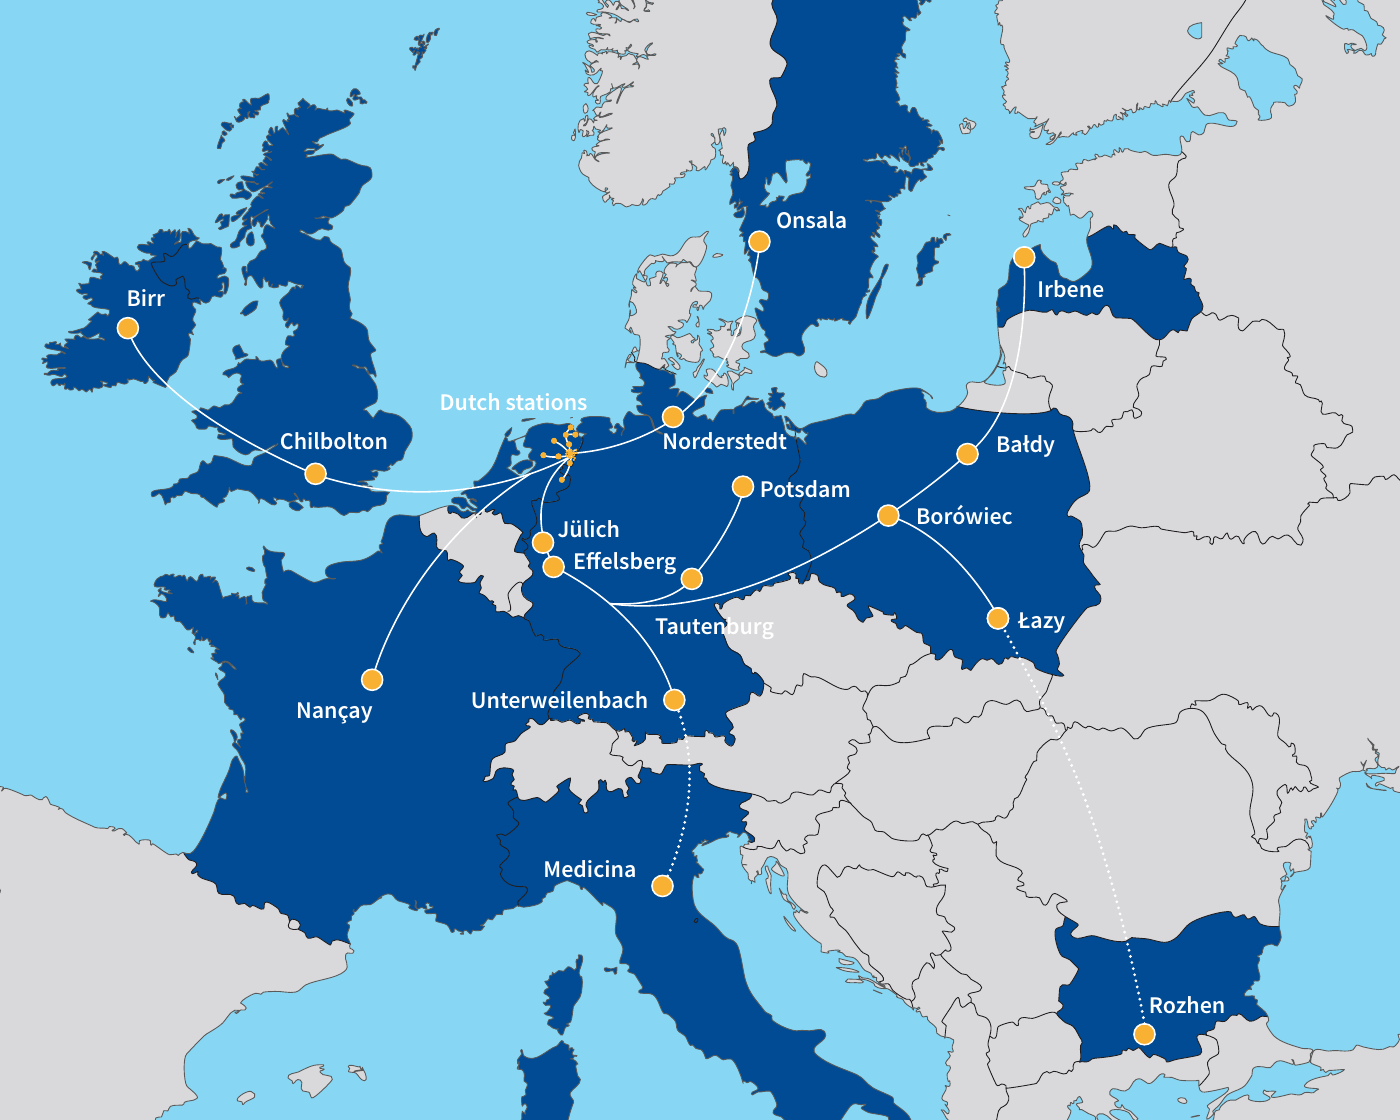
\includegraphics[width=0.9\linewidth]{img/lofar-map.png}
  \end{minipage}\hfill
  \begin{minipage}[t]{0.568\linewidth}
    \centering
    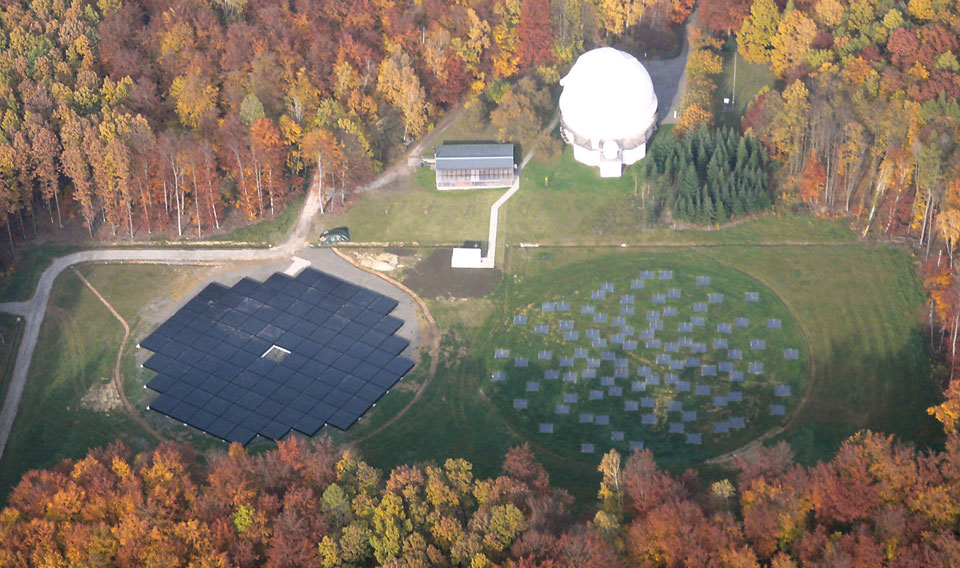
\includegraphics[width=0.9\linewidth]{img/LOFAR-station-Tautenburg1-Germany-Copyright-Michael-Pluto.png}
  \end{minipage}
  \caption[LOFAR station network and Tautenburg station]{The Dutch and international LOFAR station network map (left; map credit: ASTRON) and the LOFAR station at Tautenburg, Germany (right; photograph by Michael Pluto).}
  \label{fig:lofar_network}
\end{figure}

The LOFAR Two-metre Sky Survey (LoTSS) is the principal northern-hemisphere extragalactic survey conducted with this instrument. LoTSS observes with the High-Band Antenna from $120$ to $168\,\mathrm{MHz}$, with a central frequency of $144\,\mathrm{MHz}$. Its second data release, LoTSS-DR2, covers $5{,}634\,\mathrm{deg}^{2}$ in two contiguous regions of the northern sky at an angular resolution of $6''$, with a median rms noise of $83\,\mu\mathrm{Jy\,beam^{-1}}$, and yields a total catalogue of $4{,}396{,}228$ radio sources \citep{Shimwell2022}. At this resolution, a source with $\mathrm{LAS}=60''$ spans approximately ten synthesised beam widths, permitting resolved morphological information to be recovered, although the visibility of individual cores, lobes, hotspots, and bent tails also depends on their surface brightness and structure.

For radio-galaxy studies, catalogue components must be associated into physical radio sources and linked, where possible, to optical or infrared host galaxies. For LoTSS-DR2, these associations are provided by a value-added catalogue combining likelihood-ratio cross-matching against optical and infrared imaging, the citizen-science project Radio Galaxy Zoo: LOFAR, and direct visual inspection by domain experts \citep{Hardcastle2023}. Within the area covered by suitable optical imaging, the catalogue assigns an optical or infrared identification to $85\,\%$ of LoTSS-DR2 sources and a spectroscopic or photometric redshift to $58\,\%$. It also supplies source associations and size information needed to construct a catalogue of resolved radio galaxies.

The third data release, LoTSS-DR3, substantially extends this coverage: it contains $12{,}950\,\mathrm{h}$ of observations over $19{,}035\,\mathrm{deg}^{2}$, corresponding to $88\,\%$ of the northern sky, and catalogues $13{,}667{,}877$ radio sources at $6''$ resolution, increasing to $9''$ below declination $10^{\circ}$ \citep{Shimwell2026}. A dedicated catalogue of galaxy clusters with diffuse radio emission has also been compiled from the DR3 imaging \citep{Stuardi2026}. The catalogue-scale sample in this thesis remains based on DR2 because it was selected using the host associations and angular-size information in the DR2 value-added catalogue. We describe the precise data products and selection criteria in Chapter~\ref{sec:data}.

\subsection{Radio galaxies and the morphological taxonomy}
\label{sec:bg_taxonomy}

Radio galaxies are radio-loud active galactic nuclei whose central engines launch collimated plasma jets from the vicinity of an accreting supermassive black hole.
Synchrotron emission traces a compact radio core, the jets, and the lobes or plumes inflated where the jets deposit energy into the surrounding medium. 
Shocks near the ends of powerful jets can produce compact hotspots. Hence, the observed morphology encodes both the transport of energy by the jets and
their interaction with the gaseous environment across galactic and cluster scales \citep{HardcastleCroston2020}.
The most widely used morphological division is the Fanaroff--Riley (FR) classification. 
\citet{Fanaroff1974} defined the ratio $R_{\mathrm{FR}}$ of the separation of the highest-surface-brightness regions on opposite sides of the host, excluding the compact central core, to the total source extent.
FR\,I sources have $R_{\mathrm{FR}}<0.5$ and are centre-brightened, whereas FR\,II sources have $R_{\mathrm{FR}}>0.5$ and are edge-brightened (top-left and top-middle sources in Fig.~\ref{fig:radio_morphology_overview}). 
In the original 3CR sample, the transition occurred near a 178-MHz radio power of $P_{178}\simeq2\times10^{25}\,\mathrm{W\,Hz^{-1}\,sr^{-1}}$ under the cosmology adopted in that work. This was an empirical correlation, not a strict physical boundary. Lower-power jets are typically more susceptible to disruption and deceleration into diffuse plumes, whereas more powerful jets can remain collimated until they terminate in hotspots. Nevertheless, jet power, host-galaxy properties, and environment all influence the resulting morphology \citep{HardcastleCroston2020}.

Clearly, the radio-galaxy population is not exhausted by this binary scheme. FR\,0 sources are compact, core-dominated radio galaxies with weak or absent extended emission \citep{Baldi2015}. 
Bent-tail sources are distinguished mostly by geometry rather than by a unique formation mechanism.
Narrow-angle-tail (NAT) sources have closely swept-back jets or tails and are commonly associated with ram pressure produced by relative motion between the galaxy and the intracluster medium (ICM) (top-right source in Fig.~\ref{fig:radio_morphology_overview}).
Wide-angle-tail (WAT) sources have a broader opening angle, often with initially collimated jets that flare into bent plumes around a cluster-dominant galaxy (bottom-left in Fig.~\ref{fig:radio_morphology_overview}). Relative galaxy--ICM motion associated with cluster mergers can contribute to their bending \citep{Sakelliou2000}.
Head-tail (HT) is a broader descriptive label for emission trailing away from a bright head and does not require a single resolved tail (bottom-middle in Fig.~\ref{fig:radio_morphology_overview}). These forms encode interactions between the radio jets, the motion of the host, and the surrounding gas.
Relaxed double (RD) sources are symmetric relaxed structures, with no visible jets and less interaction with a dense environment (bottom-right in Fig.~\ref{fig:radio_morphology_overview}). The absence of compact cores, hotspots and jets suggests that these RDs represent the late evolutionary stage of radio galaxies \citep{Chilufya2025}.

\begin{figure}[ht]
  \centering
  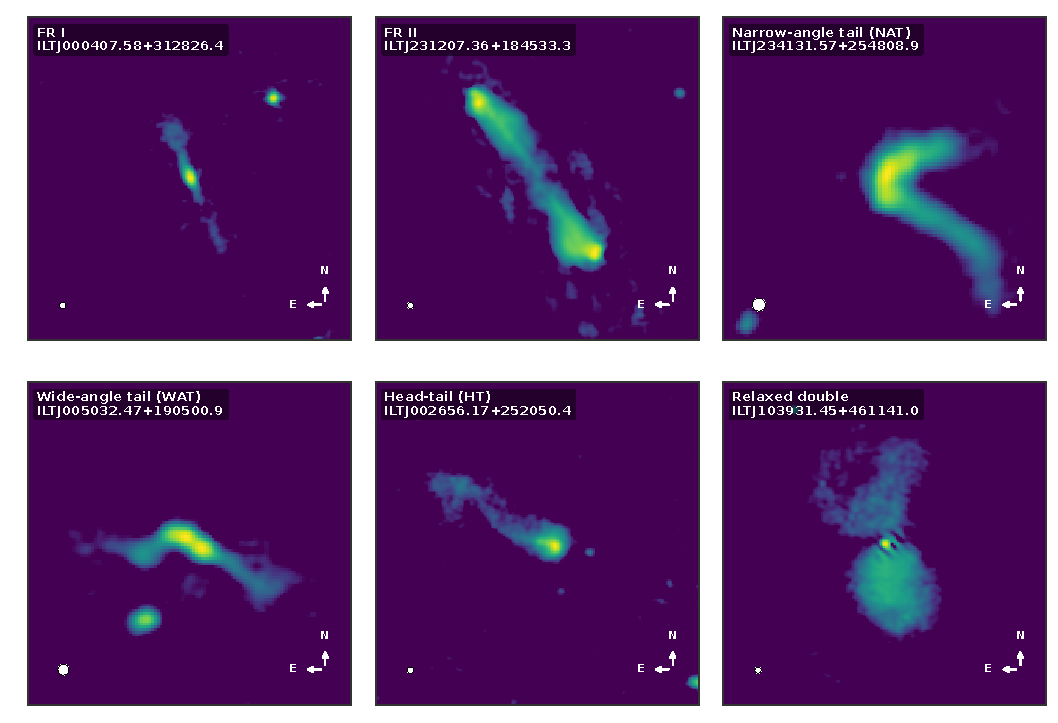
\includegraphics[width=0.9\textwidth]{img/radio_morphology_overview.pdf}
  \caption[Examples of radio-galaxy morphologies]{Representative host-centred LoTSS-DR2 144-MHz images of the radio-galaxy morphologies classified by \citet{Chilufya2025}. Each field spans $1.5\times\mathrm{LAS}$; the synthesised beam is shown at lower left, with north up and east left.}
  \label{fig:radio_morphology_overview}
\end{figure}

LoTSS has demonstrated that these morphological categories overlap strongly in their physical properties. Using $5{,}805$ extended radio-loud AGN from LoTSS-DR1, \citet{Mingo2019} found significant overlap between the FR\,I and FR\,II luminosity distributions and a population of FR\,IIs extending three orders of magnitude below the canonical FR break at $L_{150}\sim10^{26}\,\mathrm{W\,Hz^{-1}}$.
In LoTSS-DR2, \citet{Clews2025} classified $3{,}590$ FR\,IIs and $2{,}354$ FR\,Is at $z\leq0.8$. 
Near the FR divide, FR\,I morphology is more frequent in more massive hosts, but no robust correlation between the break luminosity and stellar mass remains after selection effects are considered. This dependence on multiple source and host properties reinforces that FR morphology is not determined by a single luminosity division.
\citet{Chilufya2025} studied $2{,}828$ extended radio-loud AGN with $\mathrm{LAS}>60''$ and found that almost all FR\,Is in their spectroscopic sample are low-excitation radio galaxies, whereas high-excitation objects occur predominantly among luminous FR\,IIs; nevertheless, no single radio or host property fully determines accretion mode. 
Finally, \citet{Horton2025} catalogued $9{,}985$ large, bright LoTSS-DR2 sources using broad morphologies and finer structural attributes, finding at least one possible jet-precession indicator in $28\,\%$ of the sample. 
Together, these results motivate a morphology taxonomy richer than a strict FR dichotomy.

Radio galaxies can also be distinguished by their physical scale and activity history.
For instance, giant radio galaxies have projected sizes above approximately $0.7\,\mathrm{Mpc}$; \citet{Dabhade2020} identified $239$ in LoTSS-DR1, including seven larger than $2\,\mathrm{Mpc}$.
Remnant and restarted radio galaxies instead preserve diffuse plasma from earlier episodes of jet activity, sometimes alongside newly formed jets or lobes. 
These properties can coexist with the FR and bent-tail labels and further broaden the range of radio-galaxy appearances.

Large morphology catalogues also differ in how their labels are constructed. \citet{Clews2025} used a semi-automated method based on radio-source ridgelines, whereas \citet{Horton2025} assigned detailed, multi-attribute labels through visual inspection of LoTSS images. \citet{Chilufya2025} used visual classification supported by higher-resolution VLASS observations and multiple independent classifiers. 
Differences in source selection, available image information, and classification specificity mean that these catalogues provide distinct reference schemes instead of establishing ground-truth labels.

\subsection{Diffuse radio emission in galaxy clusters}
\label{sec:bg_diffuse}

Galaxy clusters contain a hot, magnetised intracluster medium (ICM) in which relativistic electrons produce extended synchrotron emission.
This diffuse emission is not associated one-to-one with an optical galaxy and is conventionally divided into radio haloes, mini-haloes, and radio relics \citep{vanWeeren2019} (Figure~\ref{fig:cluster_diffuse_classes}).
These categories describe different locations and morphologies within a galaxy cluster. 
Interestingly, they do not imply that active galaxies are irrelevant to this emission: fossil plasma deposited by earlier AGN activity may provide seed particles that are subsequently re-energised in the ICM.

\begin{figure}[H]
  \centering
  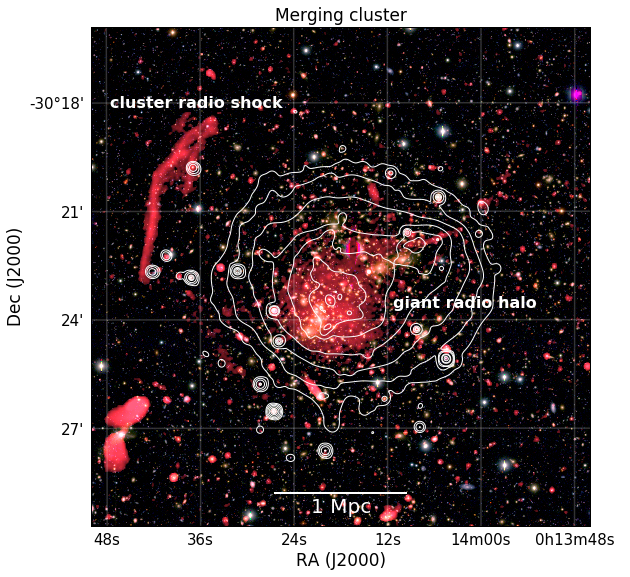
\includegraphics[width=0.45\textwidth]{img/a2744_halo_relic.png}\hfill
  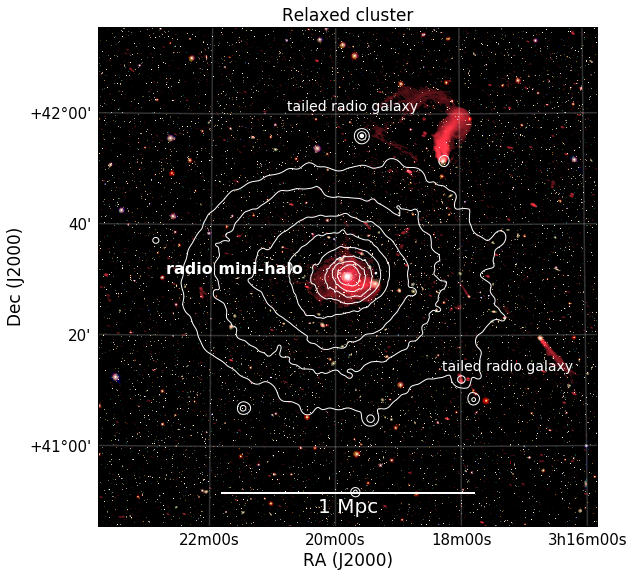
\includegraphics[width=0.45\textwidth]{img/perseus_minihalo.png}
  \caption[Examples of radio haloes, relics and mini-haloes]{Radio halo and relic emission in Abell~2744 (left) and the Perseus mini-halo (right). Reproduced from \citet{vanWeeren2019} under CC BY~4.0.}
  \label{fig:cluster_diffuse_classes}
\end{figure}

Radio relics are often elongated, arc-like sources found mainly in the periphery of merging clusters and are frequently polarised at gigahertz frequencies.
Their locations and spectral properties associate them with merger-driven shock waves, where electrons may be freshly accelerated or re-accelerated from a fossil population. Revived fossil or phoenix plasma is a related but distinct diffuse-emission category; here, relic refers to the selected elongated cluster sources \citep{vanWeeren2019}.
The northern ``Sausage'' relic in CIZA\,J$2242.8{+}5301$ is a well-studied example (Fig.~\ref{fig:sausage_relic}). It forms a thin, nearly $2\,\mathrm{Mpc}$ arc with aligned magnetic fields and a radio spectrum that steepens downstream from the outer edge \citep{vanWeeren2010}.

Radio haloes instead occupy the central regions of merging clusters, extend over scales of order a megaparsec, and broadly follow the distribution of the thermal ICM.
Turbulent re-acceleration following a merger is a leading explanation for their distributed emission.
Mini-haloes are smaller, typically spanning about $100$--$500\,\mathrm{kpc}$ around the brightest cluster galaxy in relaxed cool-core clusters.
\begin{wrapfigure}{r}{0.45\textwidth}
\vspace{-0.5cm}
  \centering
  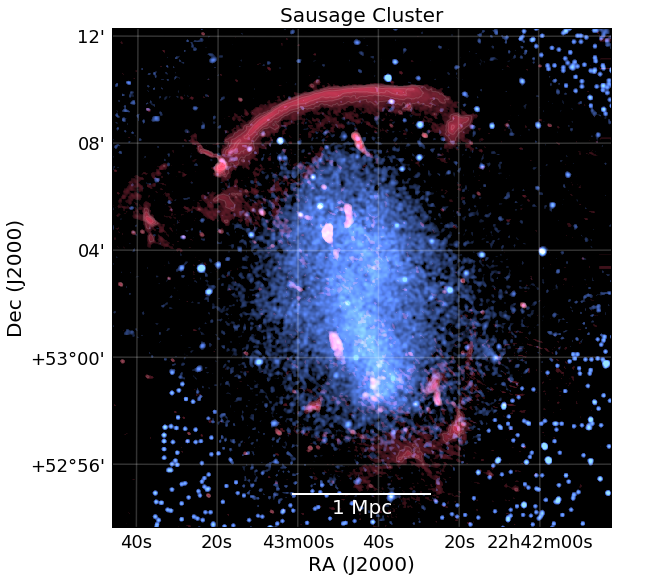
\includegraphics[width=\linewidth]{img/sausage_relic.png}
  \caption[Radio and X-ray emission in the Sausage cluster]{The Sausage cluster: 610-MHz radio (red) and X-ray (blue) emission. Reproduced from \citet{vanWeeren2019} under CC BY~4.0.}
  \label{fig:sausage_relic}
\vspace{-1cm}
\end{wrapfigure}
Sloshing-induced turbulence and re-acceleration of seed particles supplied by the central radio galaxy are among the proposed mechanisms.
Haloes and mini-haloes can contain substantial substructure, but unlike relics their emission is not localised to an identifiable peripheral shock \citep{vanWeeren2019}.

Radio relics have a different physical origin from radio galaxies, yet their diffuse structures may resemble parts of radio-galaxy emission. 
This motivates examining whether a model trained to distinguish radio-galaxy morphologies assigns similar descriptions to relics. We explore this question using selected, manually masked relic images described in Section~\ref{sec:data_relics}. Nevertheless, this test does not establish whether the model can recognise unfamiliar sources in general.

\subsection{Self-supervised representations and clustering}
\label{sec:bg_ssl}

Machine learning (ML) uses models fitted to data to recognise patterns and make predictions. In astronomy, it provides tools for analysing large survey datasets whose scale and diversity make detailed manual inspection difficult.
Deep learning is a subset of ML in which neural networks with multiple processing layers organised within a particular architecture learn successive representations of the input. For image inputs, these representations can capture spatial structure directly from pixel intensities. Applications in radio astronomy include source detection, morphological classification, and searches for similar or unusual objects~\citep{Slijepcevic2024,Riggi2024}. However, the available images greatly outnumber those with reliable expert labels, motivating methods that can learn useful representations from unlabelled observations~\citep{Slijepcevic2024}.

Supervised learning trains a model from images paired with class labels, and unsupervised learning searches for structure without such labels.
Self-supervised learning also uses unlabelled data, but constructs a training objective from the data themselves.
In this thesis, self-supervised pre-training first teaches a network to encode radio-source structure.
The pre-trained network is then fine-tuned on a smaller labelled sample for morphological classification~\citep{Nicolas2025}.

An encoder $f_\theta$ maps an input image $x$ to a finite-dimensional representation $h=f_\theta(x)$, also called an embedding. 
Distances in the embedding space express which image features the encoder regards as similar.
A morphology-aware embedding should place structurally similar radio sources close together even when their orientation or brightness differs.
Subsequently, this representation space can be clustered to construct morphological groups and used as the input to a classifier~\citep{Nicolas2025,Slijepcevic2024}.

The framework adopted by \citet{Nicolas2025} and followed here is \textit{A Simple Framework for Contrastive Learning of Visual Representations} \citep[SimCLR;][]{Chen2020}.
Two independently augmented views of each image form a positive pair.
Views originating from other images in the same minibatch act as negative examples.
These comparisons provide a supervisory signal without requiring morphology labels.
The augmentations are assumed to preserve the underlying source morphology while changing nuisance properties such as orientation or brightness. Bringing the resulting positive views together therefore teaches the encoder invariance to those transformations. A minibatch is the group of images processed together in one optimisation step.
An encoder $f_\theta$ and a projection head $g_\phi$ are trained jointly so that projected positive-pair embeddings are similar and negative-pair embeddings are separated. 
For $2N$ views generated from $N$ images, the contribution of a positive pair $(i,j)$ to the normalised temperature-scaled cross-entropy (NT-Xent) loss is
\begin{equation}
\mathcal{L}_{i,j} = -\log \frac{\exp\!\left(\mathrm{sim}(z_i,z_j)/\tau\right)}{\sum_{k=1}^{2N}\mathbf{1}_{[k\neq i]}\,\exp\!\left(\mathrm{sim}(z_i,z_k)/\tau\right)},
\label{eq:ntxent}
\end{equation}
where $z=g_\phi(f_\theta(x))$, $\mathrm{sim}(u,v)=u\cdot v/(\lVert u\rVert\lVert v\rVert)$ is cosine similarity, and $\tau$ controls how strongly the loss distinguishes similar from dissimilar embeddings.
The indicator excludes the anchor from the denominator. After pre-training, the projection head is discarded and the encoder is retained for downstream use.

For an anchor view \(i\), the numerator measures its similarity to the corresponding positive view \(j\). The denominator compares that positive similarity with the similarities between \(i\) and every other view in the minibatch, excluding only \(i\) itself. Minimising the loss therefore increases the positive pair's similarity relative to the competing views. The temperature \(\tau\) controls how strongly differences between similarities are emphasised; each of the two views is used in turn as the anchor, and the resulting contributions are averaged.

Standard SimCLR has a limitation for radio-morphology applications: views originating from other images in the minibatch are treated as negative examples.
Distinct sources with nearly identical morphology may therefore be pushed apart in the representation space.
The random structural view (RSV) introduced by \citet{Nicolas2025} addresses this limitation by allowing one augmented view to be replaced by a view of a structurally similar source identified using semi-invariant structural similarity.
Thus, positive pairs can connect distinct sources with similar morphology, encouraging the representation space to encode cross-source structural similarity.
The transformations and selection parameters used in this thesis are specified in Sec.~\ref{sec:method_simclr}.

After pre-training, the learned representations must be organised into candidate morphological groups.
Principal component analysis (PCA) projects the high-dimensional representations onto orthogonal axes ordered by the variance they explain \citep{Jolliffe2016}.
This linear construction is mathematically transparent: every principal component is a linear combination of the encoder features, its contribution is quantified by its explained variance, and the reduced dimensionality can be selected through an explicit retained-variance criterion.
Hierarchical density-based spatial clustering of applications with noise (HDBSCAN) is applied here to the retained multidimensional PCA representation.
Unlike methods that require a predetermined number of approximately spherical clusters, HDBSCAN identifies dense regions with potentially different shapes and densities and can leave isolated sources unassigned as noise \citep{Campello2013,McInnes2017}.
These properties are useful for an uncurated radio-source sample containing rare morphologies, artefacts, and ambiguous sources. 
For visualisation, the first three principal components can be plotted and coloured by the HDBSCAN assignments. 
Visual inspection of the source images within each resulting cluster then assesses morphological coherence and supports consolidation into a labelled subsample. 
The adopted PCA and HDBSCAN configuration is specified in Sec.~\ref{sec:method_simclr}.

\subsection{Deep ensembles and predictive uncertainty}
\label{sec:bg_ensembles}

The output probabilities of a single neural network by themselves can be overconfident. They do not quantify epistemic uncertainty due to training data limitations or model choice.
To increase the reliability of the probability estimates for the class predictions, \citet{Nicolas2025} adopted a deep ensemble.
\citet{Lakshminarayanan2017} proposed that training an ensemble of randomly initialised networks ($M$ classifiers with the same architecture) can yield better-calibrated probabilities and stronger out-of-distribution detection, while training and inference costs scale approximately with ensemble size.

Let $\mathbf{p}_m(x)=(p_m^c(x))_{c\in\mathcal{K}}$ denote the class-probability vector predicted for source image $x$ by ensemble member $m \in \{1,\ldots,M\}$, where $\mathcal{K}$ is the class set with cardinality $K=|\mathcal{K}|$. The ensemble mean vector $\bar{\mathbf{p}}(x)$ and ensemble agreement are defined as
\begin{equation}
\bar p^{\,c}(x) \;=\; \frac{1}{M}\sum_{m=1}^{M} p_m^c(x), \qquad
A(x) \;=\; \frac{1}{M}\sum_{m=1}^{M} \mathbf{1}\!\left[\arg\max_{c\in\mathcal{K}} p_m^c(x) = \hat{y}\right],
\label{eq:ensmean}
\end{equation}
where $A(x)\in[0,1]$ measures the fraction of ensemble members whose top-predicted class coincides with the ensemble-mean decision $\hat{y} = \arg\max_{c\in\mathcal{K}} \bar p^{\,c}(x)$. The total predictive uncertainty of the ensemble is captured by the entropy of the mean distribution,
\begin{equation}
H[\bar{\mathbf{p}}](x) \;=\; -\sum_{c\in\mathcal{K}} \bar p^{\,c}(x)\,\log \bar p^{\,c}(x),
\label{eq:H}
\end{equation}
which is maximised at $\log K$ for a uniform distribution over the $K$ classes.

\begin{table}[H]
  \centering
  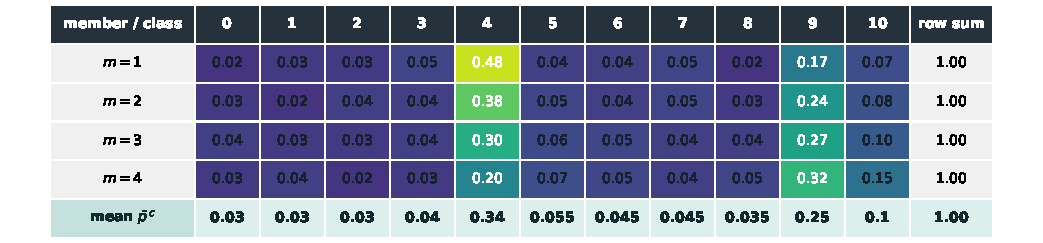
\includegraphics[width=\linewidth]{img/srg_component_walkthrough.pdf}
  \caption[Example ensemble probabilities and agreement]{Illustrative class-probability vectors for four ensemble members and their component-wise mean. Each member's predicted class is the class with the largest probability in its row, whereas the ensemble decision $\hat{y}$ is the class with the largest mean probability. Here, $\hat{y}=4$ and three of the four members also predict class~4, giving $A=3/4$. Each row sums to one.}
  \label{tab:ensemble_probability_components}
\end{table}

The total uncertainty $H[\bar{\mathbf{p}}]$ can be decomposed algebraically into terms commonly associated with the data (aleatoric) and model (epistemic) components. The model-disagreement term, commonly interpreted as epistemic uncertainty, is the mutual information ($\mathrm{MI}$) between the class prediction and the ensemble index $m$ when members are treated as uniformly sampled models. It can be expressed in closed form as the difference between the entropy of the mean and the mean of the per-member entropies \citep{Houlsby2011,Depeweg2018},
\begin{equation}
\mathrm{MI}(x) \;=\; H[\bar{\mathbf{p}}](x) \;-\; \frac{1}{M}\sum_{m=1}^{M} H[\mathbf{p}_m](x).
\label{eq:MI}
\end{equation}

All ensemble members start from the same pre-trained encoder weights and biases, which are subsequently updated during fine-tuning. The resulting independently fine-tuned members are not exact samples from a posterior distribution. Therefore, $\mathrm{MI}(x)$ is interpreted here as an empirical measure of model disagreement, not as an exact Bayesian separation of aleatoric and epistemic uncertainty.

The mutual information is bounded above by $\log K$, as is $H$. Compared to the agreement rate $A$, $\mathrm{MI}$ captures disagreement between ensemble members across the full predicted distribution.
It can therefore respond to differences that leave the top class unchanged, but it is not universally more sensitive than $A$.
Henceforth, the quantities $(A,H,\mathrm{MI})$ are used as complementary uncertainty-related inputs to define the reliability factor $R(x)$ (see Sec.~\ref{sec:method_srg}).

\cleartooddpage
\section{Data}
\label{sec:data}

Three datasets are used throughout this work: the extended LoTSS-DR2 source sample, external morphology catalogues, and selected radio-relic cutouts. This chapter describes their selection and preparation, distinguishing the images used for model training and catalogue inference from the reference data used for comparison and the diffuse-emission application.

\subsection{LoTSS-DR2 sample selection and preprocessing}
\label{sec:data_catalogue}

The main catalogue dataset consists of the two LoTSS-DR2 products introduced in Sec.~\ref{sec:bg_lotss}:
\begin{itemize}
\item the \(6''\)-resolution Stokes~I mosaics provide the image data, with their \(1.5''\) pixel sampling used to construct the cutouts \citep{Shimwell2022}; and
\item the value-added catalogue of \citet{Hardcastle2023} supplies the source identifier, resolved-source flag, optical or infrared host coordinates, largest angular size (LAS), peak flux density, and mosaic identifier.
\end{itemize}
These quantities define the sample and extraction geometry. Note that no morphology label from an external catalogue enters this stage.

We started from the \textit{resolved} sources of the value-added catalogue and applied the following filters:
\begin{itemize}
\item an angular size \(60'' \leq \mathrm{LAS} \leq 1000''\);
\item an optical or infrared host position with both coordinates available; and
\item a peak flux density of at least \(0.75\,\mathrm{mJy\,beam^{-1}}\).
\end{itemize}
The host coordinates define the centre of each cutout. Unlike \citet{Nicolas2025}, we did not impose an active-pixel selection because it would substantially reduce the sample and could preferentially remove sources whose emission is distributed across diffuse, low-surface-brightness structures. The resulting dataset contains \(32\,514\) sources and is used for representation learning and catalogue inference.

The angular-size window selects the extended-source regime motivated in Sec.~\ref{sec:bg_lotss} and complements the \(30'' < \mathrm{LAS} < 60''\) interval studied by \citet{Nicolas2025}. The upper bound of \(1000''\) limits both the downsampling required for the fixed model input size and the amount of unrelated emission in the frame. Centring each cutout on the host position rather than the radio centroid avoids systematically anchoring asymmetric sources at their brightest component \citep{Nicolas2025}.

The selected population is concentrated towards the lower ends of both the angular-size and peak-flux ranges (Fig.~\ref{fig:data_sample_distributions}).

\begin{figure}[ht]
  \centering
  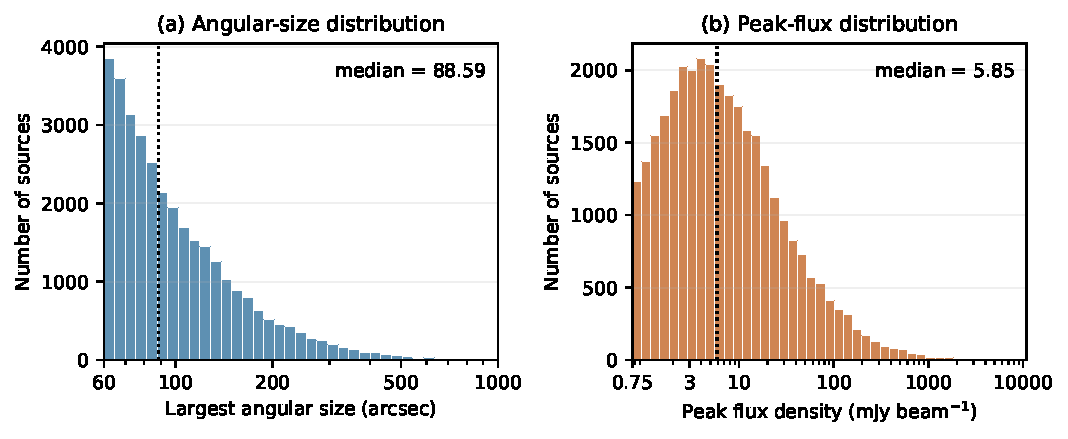
\includegraphics[width=\linewidth]{img/data_sample_distributions.pdf}
  \caption[Angular-size and peak-flux-density distributions]{Largest-angular-size and peak-flux-density distributions of the
    32\,514 sources in the processed catalogue sample. Both horizontal
    axes are logarithmic; dotted lines mark the sample medians.}
  \label{fig:data_sample_distributions}
\end{figure}

Each selected source is converted into a model input by the preprocessing pipeline of \citet{Nicolas2025}:
\begin{enumerate}
\item A square cutout of side \(1.5\times\mathrm{LAS}\) is extracted from the corresponding mosaic and centred on the host position.
\item Pixel values below \(v_{\min}=3\sigma_{\mathrm{img}}\) are set to \(v_{\min}\), where \(\sigma_{\mathrm{img}}\) is the sigma-clipped standard deviation of the cutout, estimated with a \(3\sigma\) rejection threshold and at most ten iterations. This suppresses background fluctuations and low-intensity artefacts.
\item The clipped image is then resampled to \(128\times128\) pixels using scikit-image's default first-order interpolation for floating-point arrays, min--max normalised to \([0,1]\), and stored as an 8-bit single-channel greyscale image.
\end{enumerate}
Because the cutout side scales with the LAS, sources of very different angular size appear at a comparable scale in the frame, so that the network input is dominated by morphology.

\begingroup
\emergencystretch=2em
The model receives linearly min--max-normalised intensities. For visual inspection, the representative-source galleries use a symmetric-logarithmic intensity display to reveal faint structure. Only the archived raw-cluster panels retain their original display scaling.
\par
\endgroup

\subsection{External reference catalogues}
\label{sec:data_external}

We used three independently constructed morphological catalogues (Table~\ref{tab:external_individual_samples}) of LoTSS-DR2 sources exclusively for comparison (Sec.~\ref{sec:results_external}).
\begin{table}[h]
\centering
\small
\setstretch{1}
\setlength{\tabcolsep}{4pt}
\renewcommand{\arraystretch}{1.25}
\begin{tabular*}{\linewidth}{@{}p{0.15\linewidth}@{\extracolsep{\fill}}p{0.35\linewidth}rrrr@{}}
\toprule
Catalogue & Description & \shortstack[r]{Full\\catalogue} & Matched & Mapped & \shortstack[r]{Mapped,\\curated\\excluded} \\
\midrule
\raggedright\citet{Clews2025} & \raggedright Semi-automated ridgeline analysis covering classical radio-galaxy morphologies. & 20\,172 & 11\,062 & 8\,402 & 7\,757 \\
\addlinespace
\raggedright\citet{Horton2025} & \raggedright Visual inspection with multi-attribute labels, including hybrid and precession-related signatures. & 9\,985 & 9\,287 & 9\,070 & 8\,352 \\
\addlinespace
\raggedright\citet{Chilufya2025} & \raggedright Classification of extended radio-loud AGN selected with \(\mathrm{LAS}>60''\). & 2\,828 & 2\,788 & 2\,788 & 2\,590 \\
\bottomrule
\end{tabular*}
\caption[Individual reference-catalogue selections]{Reference catalogues and source counts after identifier matching, morphology mapping and exclusion of internally curated sources.}
\label{tab:external_individual_samples}
\end{table}

Firstly, we cross-compared each catalogue with our primary dataset by matching their \texttt{Source\_Name} identifiers. These are flagged as \textbf{Matched} in Table~\ref{tab:external_individual_samples}.
We then translate the reference labels into our morphology classes using the rules in Sec.~\ref{sec:method_external_mapping}, retaining sources with usable labels as the \textbf{Mapped} sample.
Reference labels come from Clews's \texttt{Morph}, Horton's boolean flags and Chilufya's \texttt{Final\_Morph} (\nolinkurl{radio_optical_class-v1}).
In Sec.~\ref{sec:results_external}, we report \(F_1\) first for the \textbf{Mapped, curated excluded} samples, which remove overlap with supervised training, and then for the full \textbf{Mapped} samples.

Besides individual usage of these three catalogues, we used sources with identical mapped labels in all three catalogues. Table~\ref{tab:external_combined_samples} details each sample and its purpose.  

\begin{table}[H]
\centering
\small
\setstretch{1}
\setlength{\tabcolsep}{4pt}
\renewcommand{\arraystretch}{1.25}
\begin{tabular*}{\linewidth}{@{}p{0.26\linewidth}@{\extracolsep{\fill}}rp{0.60\linewidth}@{}}
\toprule
Sample & Sources & Definition \\
\midrule
At least one mapped reference & 16\,177 & Unique study sources with a usable label in at least one catalogue; used for score distributions. \\
Common-source sample & 404 & Study sources present in all three catalogues, regardless of label availability. \\
Common mapped sample & 311 & Common sources with usable mapped labels in all three catalogues. \\
Consensus sample & 149 & Common mapped sources assigned the same morphology by all three catalogues. \\
Consensus excluding curated sources & 139 & Consensus sources remaining after removing the internally curated sample. \\
\bottomrule
\end{tabular*}
\caption[Combined reference-catalogue selections]{Definitions and source counts for combined reference-catalogue selections.}
\label{tab:external_combined_samples}
\end{table}

\subsection{Radio-relic reference sample}
\label{sec:data_relics}

For the diffuse-emission application in Sec.~\ref{sec:method_relics}, we select ten radio relics from a yet-unpublished catalogue compiled by The Tautenburg Radio Relic Collection team under the supervision of Prof. Dr. Matthias Hoeft. Table~\ref{tab:relic_sample} lists their relic-centred coordinates and largest angular sizes (LAS), which we use directly to construct the cutouts from LoTSS-DR3. Their host clusters and the reference positions are also provided for identification.

\begin{table}[H]
\centering
\small
\setlength{\tabcolsep}{3pt}
\renewcommand{\arraystretch}{1.1}
\begin{tabular}{@{}lrrrlrr@{}}
\toprule
 & \multicolumn{2}{c}{Relic position} & & & \multicolumn{2}{c}{Cluster position} \\
\cmidrule(lr){2-3}\cmidrule(l){6-7}
Relic & RA & Dec & LAS & Host cluster & RA & Dec \\
\midrule
P113 N      & 4.9363 & 25.3543 & 228 & PSZ2 G113.91-37.01 & 4.9129 & 25.2908 \\
Toothbrush D & 90.9042 & 42.1708 & 66 & RX J0603.3+4214 & 90.825 & 42.2333 \\
Toothbrush B & 90.8333 & 42.3083 & 474 & RX J0603.3+4214 & 90.825 & 42.2333 \\
MS1752 SW   & 267.9745 & 44.6325 & 192 & MACS J1752.0+4440 & 268.009 & 44.6773 \\
MS1752 NE   & 268.0829 & 44.6953 & 270 & MACS J1752.0+4440 & 268.009 & 44.6773 \\
Zw2341 RS   & 355.95 & 0.23 & 216 & ZwCl 2341.1+0000 & 355.919 & 0.3053 \\
P096p N     & 284.1583 & 66.4417 & 204 & PSZ1 G096.89+24.17 & 284.16 & 66.3861 \\
P096p S     & 284.1875 & 66.3292 & 330 & PSZ1 G096.89+24.17 & 284.16 & 66.3861 \\
P116 N      & 8.0645 & 18.1766 & 103.8 & PSZ2 G116.50-44.47 & 8.0342 & 18.1069 \\
A2256 R1    & 256 & 78.7667 & 600 & Abell 2256 & 255.9064 & 78.623 \\
\bottomrule
\end{tabular}
\caption[Selected radio relics and host clusters]{Selected relics and their host clusters. Coordinates are in degrees and LAS in arcseconds.}
\label{tab:relic_sample}
\end{table}

We note that the original FITS headers give a circular \(9''\) beam for Zw2341 RS and \(6''\) beams for the other nine selected cutouts. Nevertheless, the relic inputs share the final pixel dimensions, not a uniform native angular resolution.

\cleartooddpage
\section{Methodology}
\label{sec:method}

This chapter describes the classification and similarity-scoring pipeline adapted from \citet{Nicolas2025} for the extended-source sample introduced in Chapter~\ref{sec:data}. We first learn image representations through SimCLR pre-training with random structural views, then use PCA, HDBSCAN, visual inspection and SI-SSIM filtering to construct eleven morphology classes (Secs.~\ref{sec:method_simclr}--\ref{sec:method_labels}). These labels support supervised fine-tuning of a 50-member ensemble (Sec.~\ref{sec:method_classifier}), whose probabilities and uncertainty measures define the similarity-to-radio-galaxy score \(S_\mathrm{RG}\) (Sec.~\ref{sec:method_srg}). We then establish the external-label mappings and evaluation metrics used to compare classifications (Sec.~\ref{sec:method_external_mapping}). Finally, we describe the masking and preprocessing of selected radio-relic cutouts to examine the ensemble's response to diffuse emission (Sec.~\ref{sec:method_relics}).

\subsection{Model Pre-training}
\label{sec:method_simclr}

The SimCLR framework with RSV introduced in Sec.~\ref{sec:bg_ssl} was implemented using the GreyResNet18 architecture.
GreyResNet18 is a ResNet-18 \citep{He2016} adapted for single-channel input, with its classification layer removed and
an input batch-normalisation (BN) layer whose affine parameters are disabled. Each \(128 \times 128\) cutout is mapped to a \(512\)-dimensional representation.
The projection head maps this representation through a \(512\)-dimensional linear layer, BN, and a rectified linear unit (ReLU), followed by a linear map to \(256\) dimensions.
The detailed architecture is shown in Appendix~\ref{app:greyresnet18_architecture}.

For each source, the augmentation pipeline independently generated two views using a random rotation through a continuous angle, a random vertical flip,
brightness jitter with a factor between \(0\) and \(1.1\), and a random resized crop retaining between \(90\,\%\) and \(100\,\%\) of the image area.
RSV subsequently modified the pool of second views before the positive pairs were passed to the encoder.

\paragraph{Random structural view via SI-SSIM.}
The semi-invariant structural similarity (SI-SSIM) between two images is the maximum structural similarity index \citep[SSIM;][]{Wang2004} obtained over the eight square-image symmetry transforms of the second image: rotations by multiples of \(90^{\circ}\), with and without a reflection. This construction is invariant to those eight transforms, rather than to arbitrary orientations, while preserving sensitivity to image structure. SI-SSIM is not scale invariant. A symmetric SI-SSIM matrix is precomputed once from cutouts downsampled to \(64 \times 64\) pixels and is reused for both RSV and the label-construction procedure of Sec.~\ref{sec:method_labels}.

For a source \(i\), the stored matrix is first restricted to the current minibatch and sorted by decreasing SI-SSIM. The implemented candidate set is

\[
\mathcal{C}_i=\{i,n_{i,1},n_{i,2},n_{i,3}\}, \qquad |\mathcal{C}_i|=k_{\mathrm{RSV}}=4.
\]

The first candidate is the original source because the matrix diagonal is one. The remaining three candidates are different sources in the minibatch rather than augmentations of the query.
One candidate is drawn uniformly, and the query's second augmented view is replaced by the independently augmented second view associated with that candidate.
Selecting the self-candidate therefore retains a standard same-source SimCLR pair, whereas selecting one of the other three candidates forms a cross-source positive pair. The nominal probability of forming a cross-source pair is \((k_{\mathrm{RSV}}-1)/k_{\mathrm{RSV}}=3/4\). Figure~\ref{fig:simclr_rsv_schematic} illustrates this selection rule and the shared SimCLR path.
\begin{figure}[H]
  \centering
  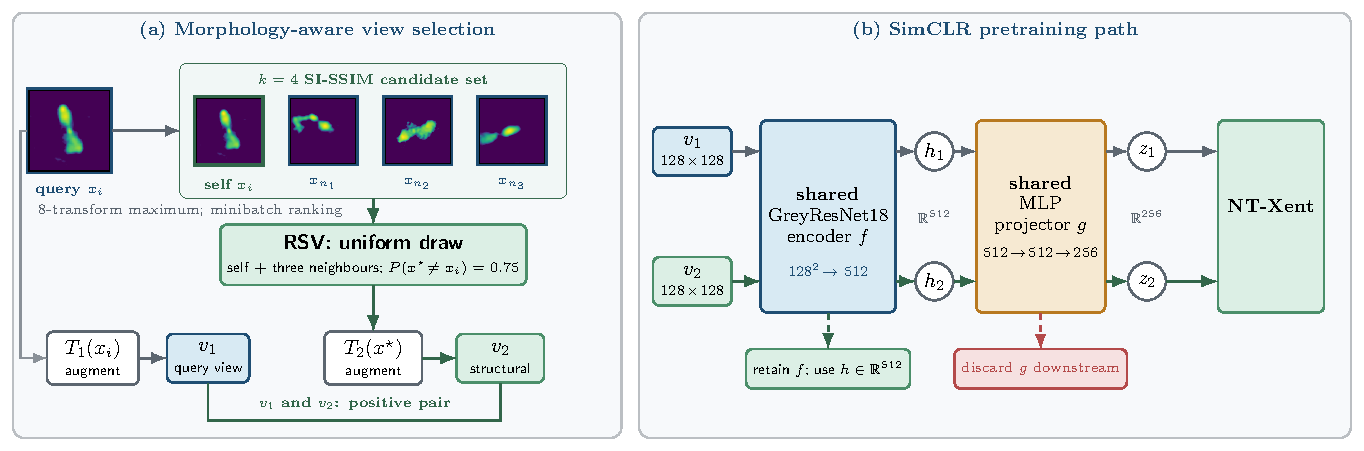
\includegraphics[width=\linewidth]{img/simclr_rsv_schematic.pdf}
  \caption[SimCLR pre-training with random structural views]{SimCLR pre-training with random structural views (RSV), adapted
    conceptually from \citet{Nicolas2025}. (a) RSV uses an independently
    augmented view of either the query or one of its three nearest SI-SSIM
    neighbours in the minibatch as the second view. (b) Both views pass through
    the shared encoder \(f\) and projector \(g\). NT-Xent is evaluated in the
    \(256\)-dimensional projection space; the \(512\)-dimensional encoder
    representation is retained downstream.}
  \label{fig:simclr_rsv_schematic}
\end{figure}

The encoder and projector were trained for \textbf{\(205\) epochs} with a \textbf{batch size of \(512\)}, AdamW \citep{Loshchilov2019}, a base \textbf{learning rate of \(3\times10^{-4}\)}, and a \textbf{weight decay of \(10^{-4}\)}. A five-epoch linear warm-up was followed by cosine annealing to one fiftieth of the base rate; training used mixed-precision arithmetic and gradient clipping at unit norm. The projection head was discarded after pre-training, and all downstream steps used the \(512\)-dimensional encoder representations.

\citet{Nicolas2025} report that removing RSV prevented the recovery of one-third of the reported morphology classes. We therefore applied RSV directly without independently assessing its effect.

The encoder and projection head were optimised with the NT-Xent objective defined in Eq.~\ref{eq:ntxent}.
Its temperature, \(\tau=0.15\), was selected empirically from a sweep of twenty runs spanning \(0.05\)--\(1.05\).
Model selection jointly favoured runs that required more principal components to retain \(90\,\%\) of the representation variance,
produced more HDBSCAN clusters, and assigned fewer sources to noise.
The selected run retained \textbf{\(15\) components}, yielded \textbf{\(59\) non-noise clusters}, and assigned \(27\,275\) sources to the noise label.

For the clustering-based evaluation described above, the \(\ell_2\)-normalised representations of all \(32\,514\) pre-training sources were reduced by
principal component analysis \citep{Jolliffe2016}. HDBSCAN \citep{Campello2013,McInnes2017} was then applied with a minimum cluster size of \(19\),
a minimum-samples value of \(1\), and the Manhattan metric. Of the full sample, \(5\,239\) sources (\(16.1\,\%\)) received non-noise labels.
The non-noise cluster sizes range from \(19\) to \(1\,502\) sources and are strongly imbalanced (Figure~\ref{fig:hdbscan_cluster_distribution}).
The three largest clusters, labels 52, 55, and 58, contain \(3\,273\) sources, or \(62.5\,\%\) of all non-noise memberships.
\begin{figure}[H]
  \centering
  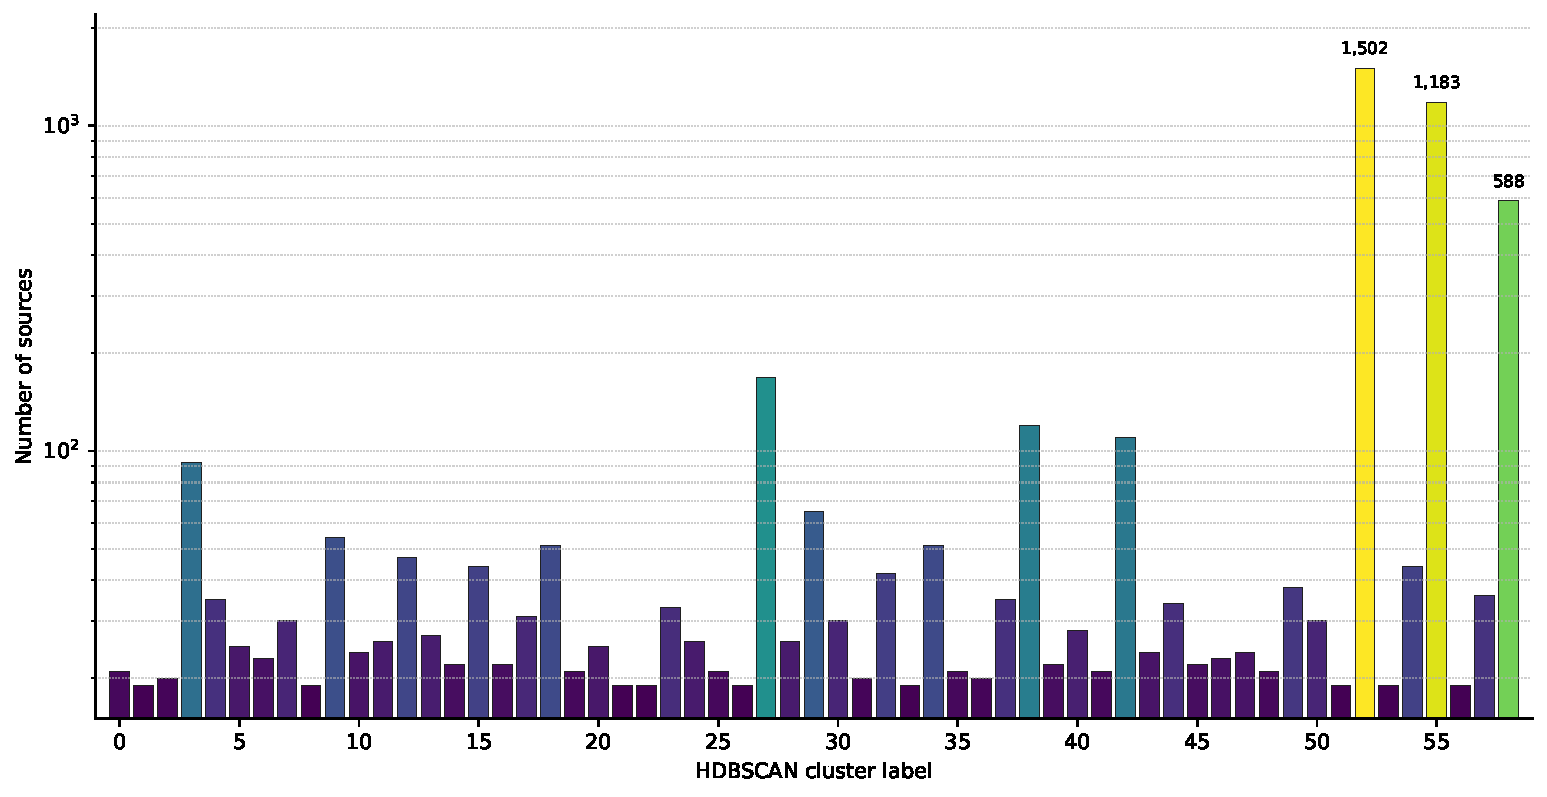
\includegraphics[width=0.85\linewidth]{img/hdbscan_cluster_distribution.pdf}
  \caption[HDBSCAN cluster membership distribution]{Membership of the 59 non-noise HDBSCAN clusters obtained using the 15 principal components that retain 90\,\% of the variance. The vertical axis is logarithmic, and the colour scale
encodes cluster size.}
  \label{fig:hdbscan_cluster_distribution}
\end{figure}

Figure~\ref{fig:hdbscan_cluster_examples} shows four randomly drawn members from six raw clusters, selected to illustrate the range of compact, elongated, bent,
and multi-component structures. These (pre-)labels denote density-based groups in the learned representation space rather than physical morphology classes.
The complete raw-cluster overview, including the noise group (cluster label -1), is provided in Appendix~\ref{app:hdbscan_cluster_overview}.
\begin{figure}[H]
  \centering
  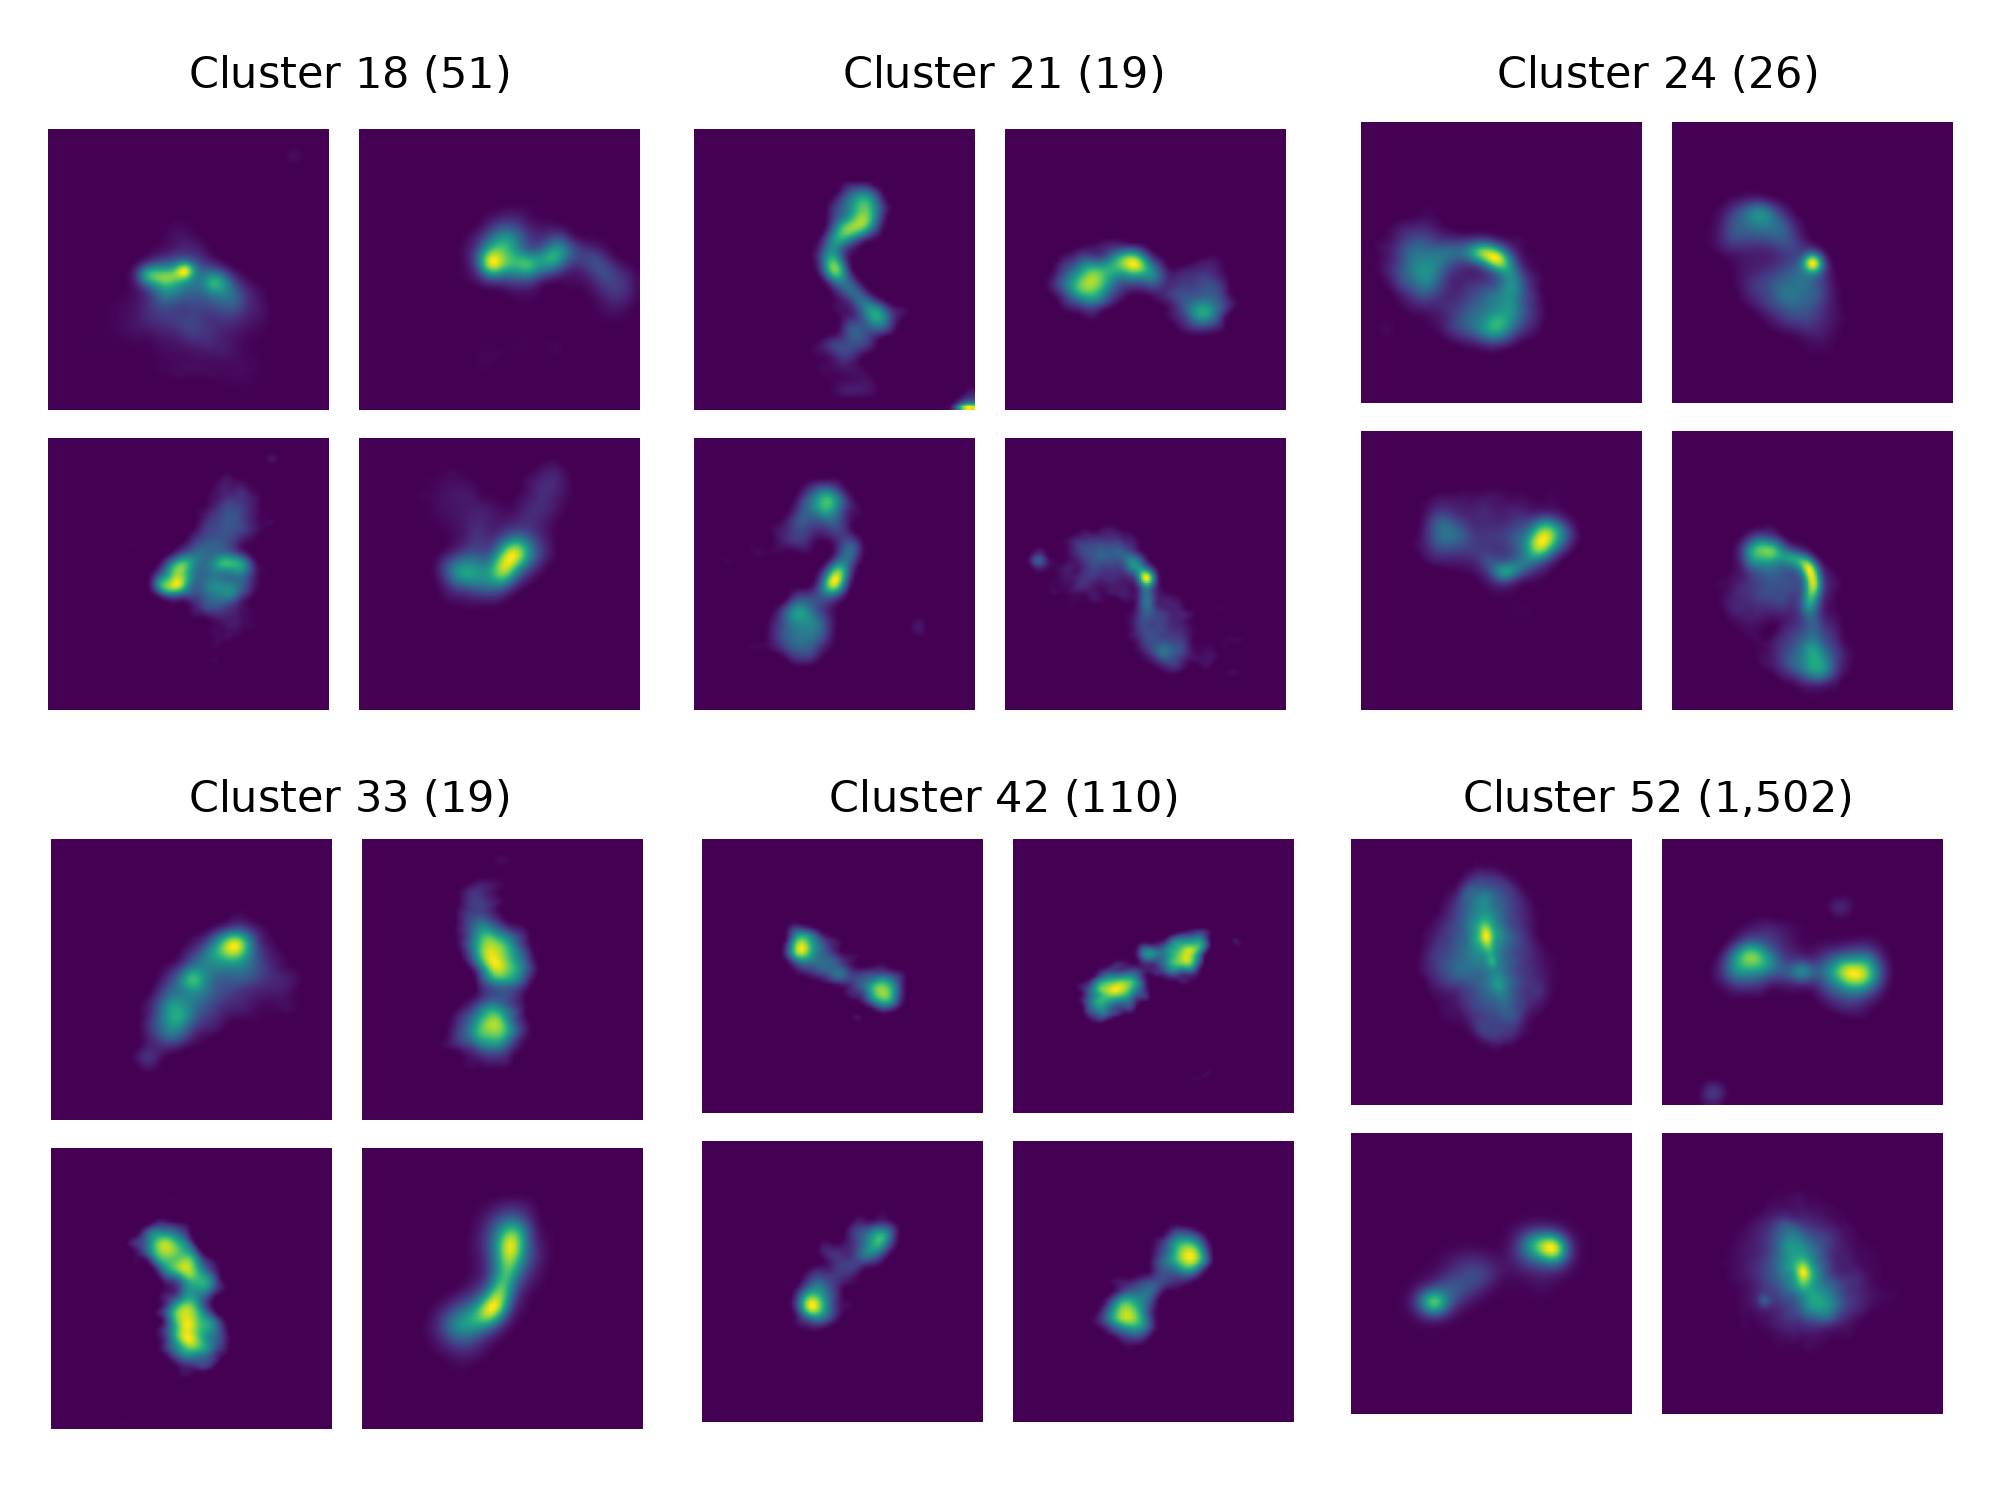
\includegraphics[width=0.85\linewidth]{img/hdbscan_cluster_examples.png}
  \caption[Examples of six raw HDBSCAN clusters]{Six raw HDBSCAN clusters. The headings are the original HDBSCAN labels with the total membership of each cluster.}
  \label{fig:hdbscan_cluster_examples}
\end{figure}

\subsection{Cluster-based class construction}
\label{sec:method_labels}

At this stage, we derive the internal taxonomy from the clustered representations that form the basis of the labels used to fine-tune the classifier.

First, each raw cluster is inspected visually. Clusters representing the same visual morphology are merged,
while clusters unsuitable for the internal taxonomy are returned to the unassigned pool.
This consolidation assigns \(3\,456\) sources to the eleven morphology classes defined below:
\begin{itemize}[leftmargin=*]
\item \textbf{Amorphous:} diffuse, extended emission without clearly defined jets, lobes, or hotspots.
\item \textbf{Asymmetric core-jet (ACJ):} a bright central component with predominantly one-sided extended emission.
\item \textbf{Bright-core:} compact, centrally peaked emission dominated by a bright core, with faint or absent extended structure.
\item \textbf{Centre-bright (FRI):} two-sided, FRI-like emission concentrated towards the centre and fading outwards.
\item \textbf{Core-Displaced:} extended emission containing a dominant compact component offset from the centroid of the resolved structure.
\item \textbf{Edge-bright (FRII) linear:} approximately collinear, FRII-like emission with brightness peaks near the outer edges.
\item \textbf{Hybrid (FRX) unclear:} mixed or ambiguous brightening patterns that do not admit a clear FRI or FRII assignment.
\item \textbf{Large FRII:} large-angular-extent, edge-bright FRII-like emission.
\item \textbf{Spirals:} extended disc- or spiral-like radio emission rather than a jet-and-lobe morphology.
\item \textbf{Structured-Bent:} resolved multi-component emission following a curved or bent axis.
\item \textbf{Unresolved:} point-like or marginally resolved emission in the normalised cutout.
\end{itemize}
These classes are operational descriptions of appearance in the normalised LoTSS-DR2 cutouts and do not constitute independently verified physical classifications.

Next, to reduce the propagation of atypical cluster members into the classifier, we compute the mean SI-SSIM of each source relative to the other members of its assigned class.
Figure~\ref{fig:class_grid} shows the seven highest-ranked sources in each class before filtering, together with their mean SI-SSIM values.
The most mutually similar \(80\,\%\) are retained by default, with class-specific retention fractions between \(60\) and \(90\,\%\) selected according to visual homogeneity.
The resulting labelled subsample is presented in Table~\ref{tab:labelled_subsample}.
The class-balanced split, shared by all ensemble members, assigns \(2\,602\), \(22\) and \(33\) sources to training, validation and testing, respectively.
The smallest class is divided approximately \(70/15/15\). Every larger class contributes the same numbers of validation and test sources, with all remaining members used for training. This produces class-balanced validation and test sets, although their small sizes prevent reliable estimation of per-class performance.
The validation and test sources also participated in self-supervised pre-training.
Sources outside the labelled subsample enter the classifier only during inference (Sec.~\ref{sec:results_classification}).

\begin{table}[H]
\centering
\begin{tabular}{lrr}
\toprule
Class & Sources & Retained (\%) \\
\midrule
Amorphous & 17 & 80 \\
Asymmetric core-jet (ACJ) & 38 & 80 \\
Bright-core & 946 & 80 \\
Centre-bright (FRI) & 267 & 80 \\
Core-Displaced & 16 & 80 \\
Edge-bright (FRII) linear & 437 & 80 \\
Hybrid (FRX) unclear & 67 & 90 \\
Large FRII & 72 & 80 \\
Spirals & 96 & 80 \\
Structured-Bent & 268 & 90 \\
Unresolved & 433 & 60 \\
\midrule
Total & 2\,657 & \\
\bottomrule
\end{tabular}
\caption[Labelled subsample and SI-SSIM retention fractions]{Labelled subsample produced by cluster-based label construction: sources retained per class and class-specific SI-SSIM retention fraction.}
\label{tab:labelled_subsample}
\end{table}

Figure~\ref{fig:curated_pca_3d} visualises how the curated morphology classes are arranged within the pre-trained representation space and relative to the unassigned sources.
Their partial concentration shows that the encoder captures morphology-related structure, while overlaps indicate that the first three PCs,
which retain \(48.81\,\%\) of the curated-subset variance, do not fully separate the classes. This descriptive projection was not used for class construction.

\begin{figure}[H]
  \centering
  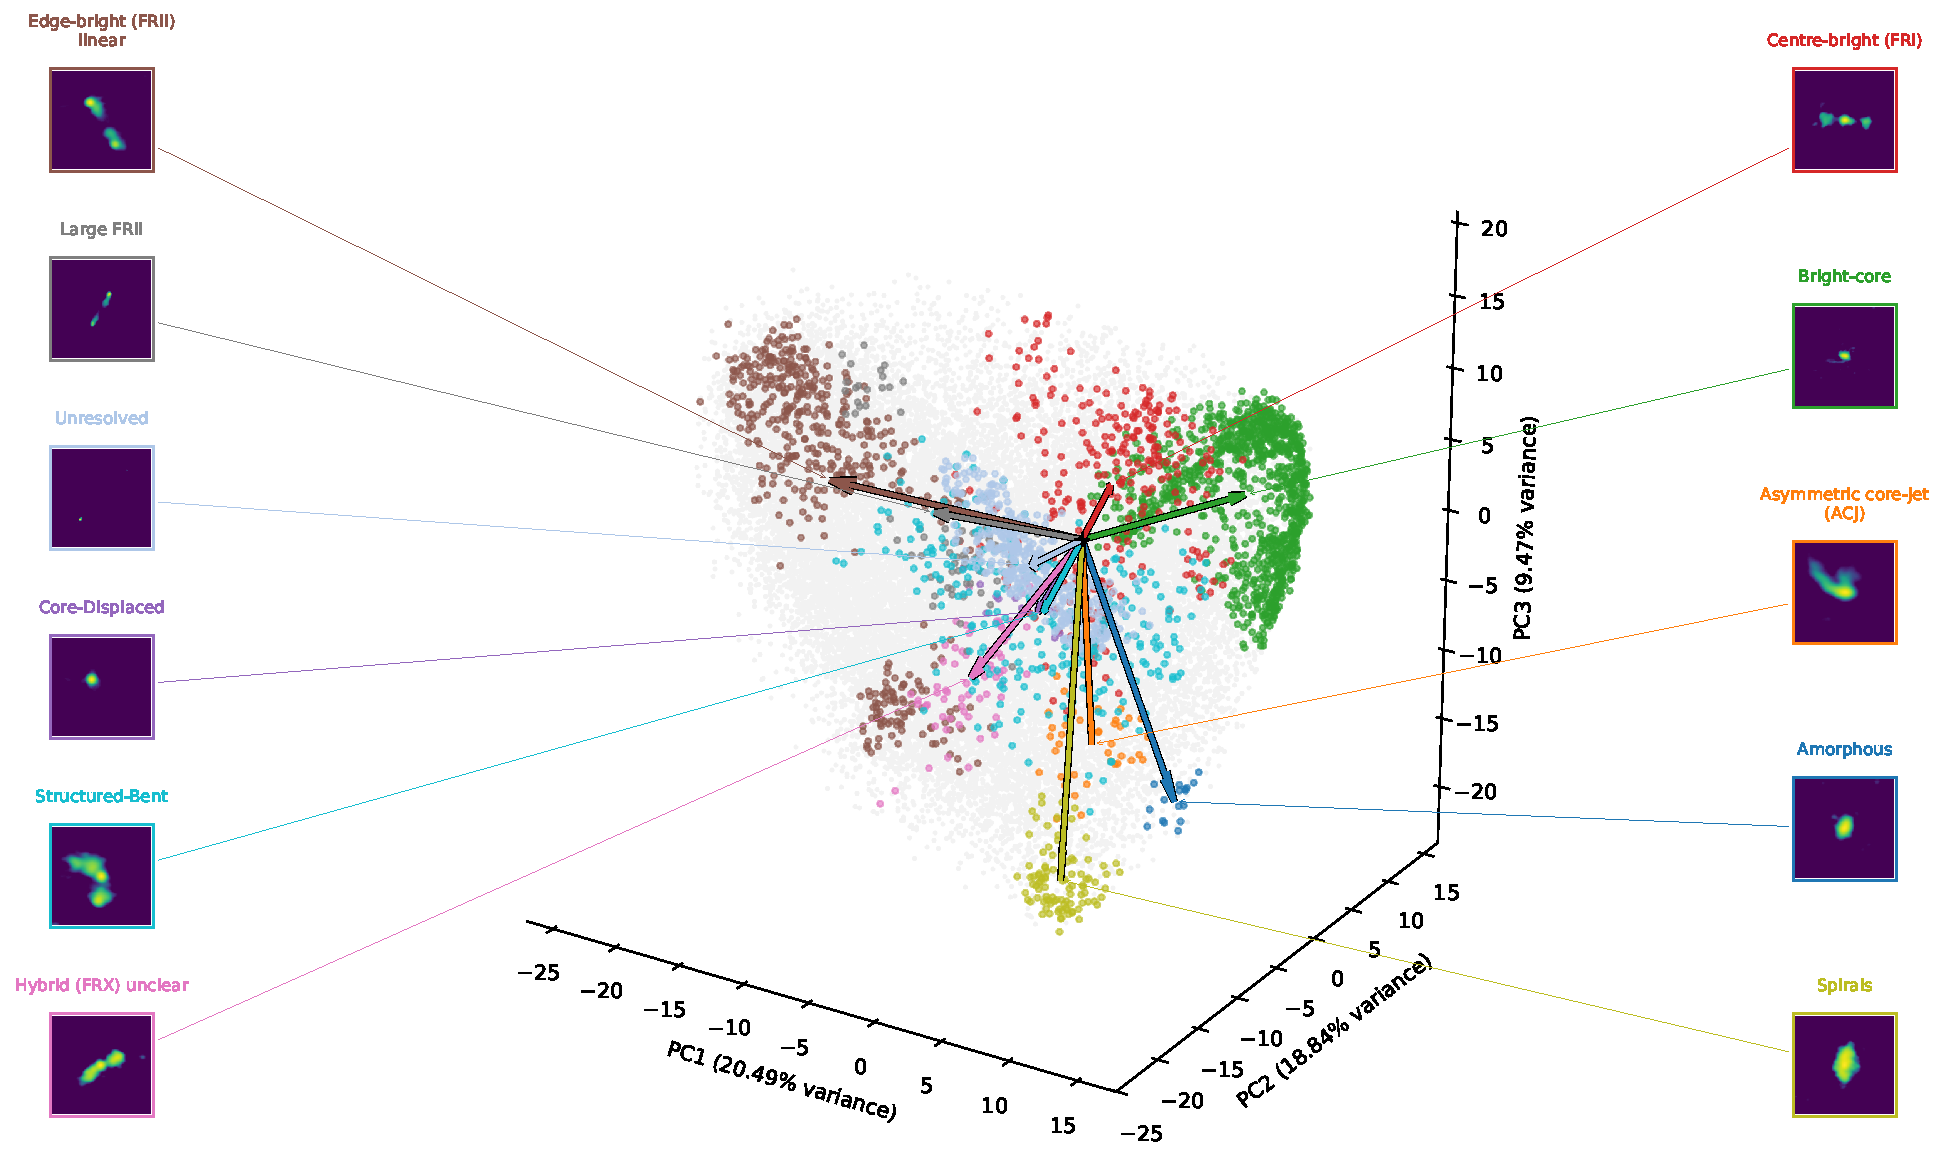
\includegraphics[width=\linewidth]{img/curated_pca_3d.pdf}
  \caption[PCA projection of curated classes and unassigned sources]{Three-dimensional PCA projection of the curated morphology classes
    and unassigned sources.}
  \label{fig:curated_pca_3d}
\end{figure}

\begin{figure}[H]
  \centering
  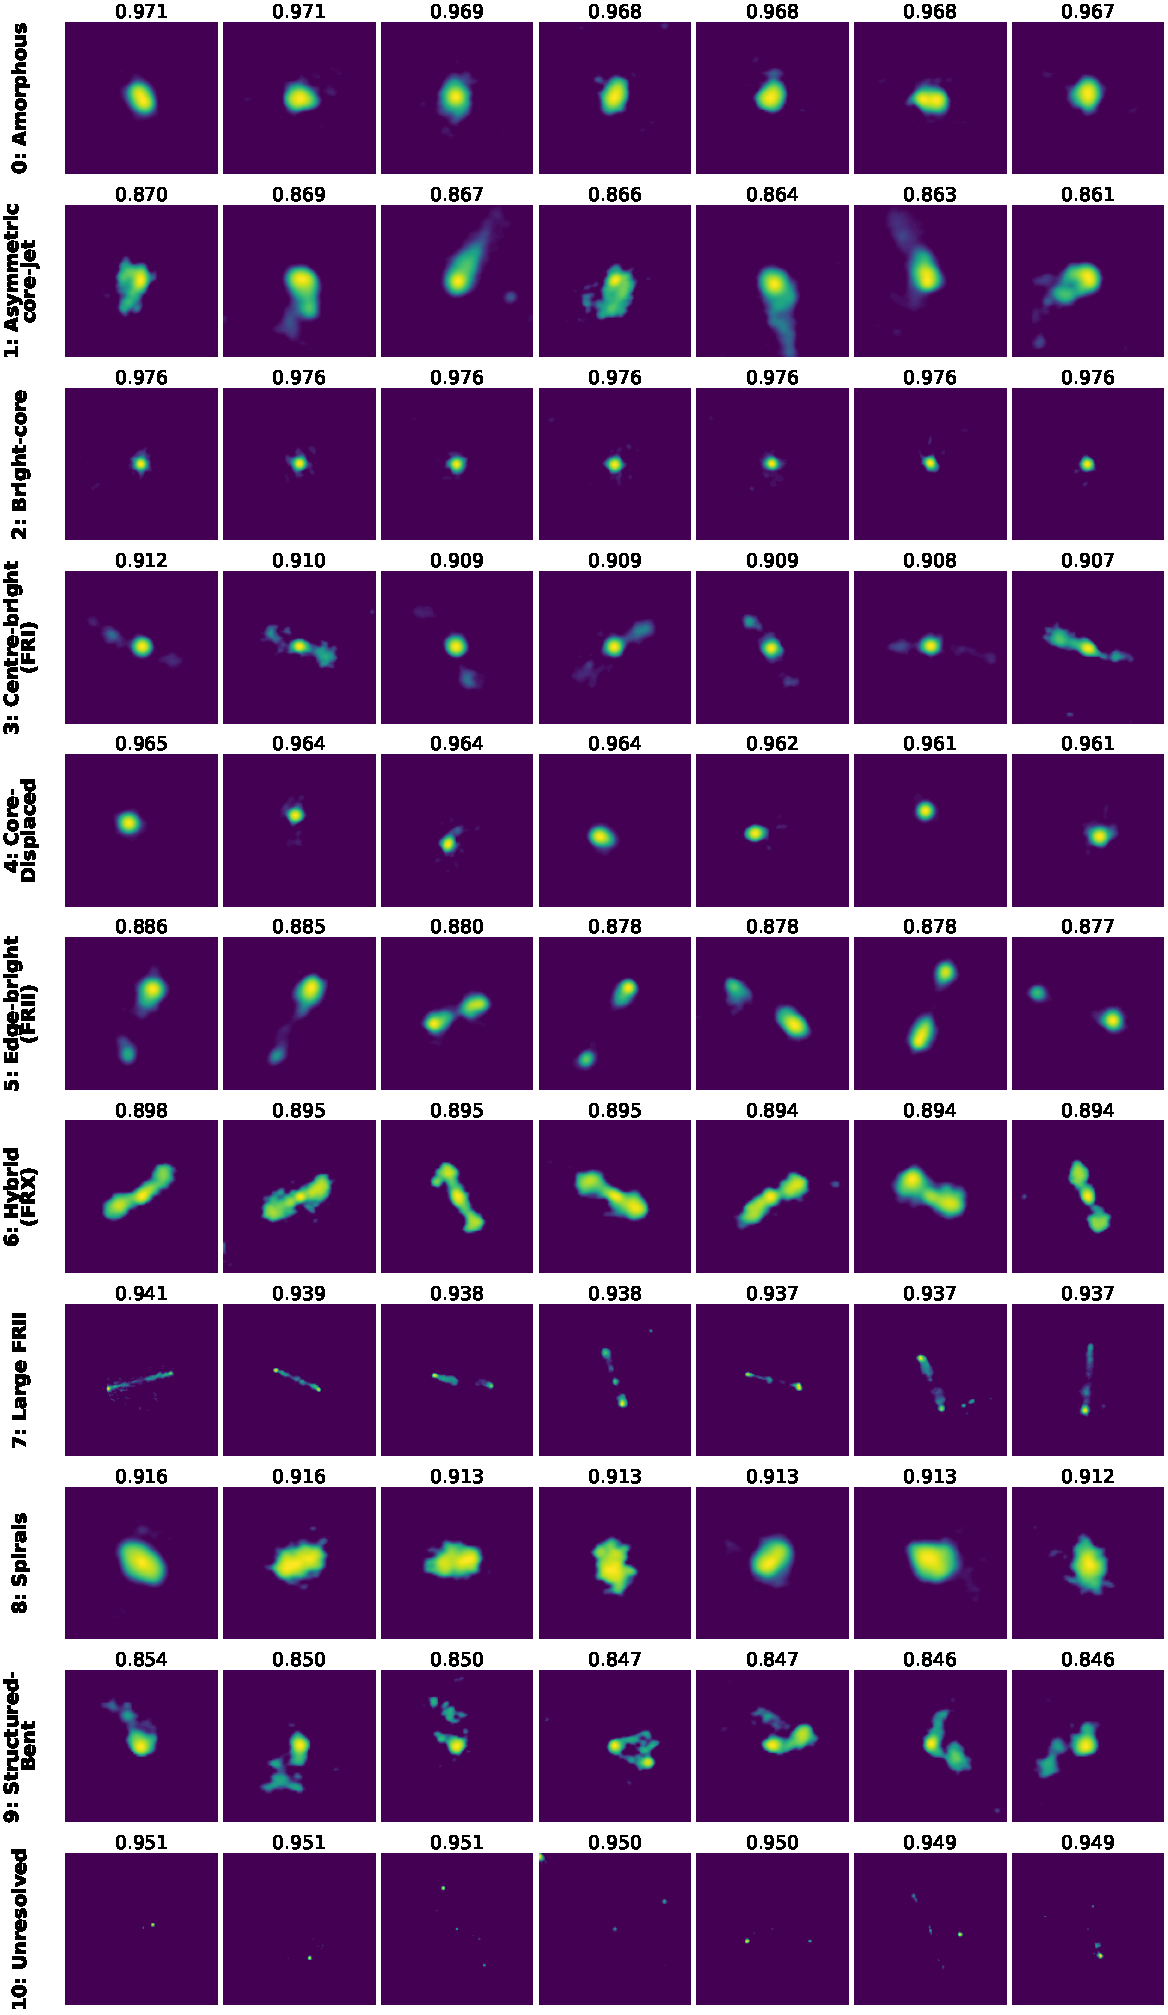
\includegraphics[width=\linewidth,height=0.9\textheight,keepaspectratio]{img/class_grid.pdf}
  \caption[Examples of the eleven internal morphology classes]{Representative LoTSS-DR2 cutouts for the eleven morphology classes.
    Each row shows the seven pre-filter sources with the highest mean within-class SI-SSIM.}
  \label{fig:class_grid}
\end{figure}

\subsection{Supervised classifier and deep ensemble}
\label{sec:method_classifier}

At this stage, with the curated morphology classes already defined, the projector is discarded and a classification head is attached to the pre-trained encoder.
The classifier maps the \(512\)-dimensional representation to eleven class logits\footnote{Unnormalised class scores converted to probabilities by the softmax function.}. We fine-tune both the encoder and the head on the labelled subsample.

The fine-tuning loss function (for a minibatch of \(B\) sources) combines two terms:
\begin{itemize}
\item \textbf{Cross-entropy} loss $\mathcal{L}_{\mathrm{CE}}$, which rewards correct class predictions \citep{Salakhutdinov2007}: 
\begin{equation}
\mathcal{L}_{\mathrm{CE}}
=-\frac{\sum_{i=1}^{B}w_{y_i}\log p_{i,y_i}}
{\sum_{i=1}^{B}w_{y_i}},
\label{eq:classifier_ce}
\end{equation} 
where \(p_{i,y_i}\) is the predicted probability of source \(i\)'s assigned class \(y_i\).
The inverse-frequency weights are \(w_c=N_{\mathrm{train}}/(K n_c)\), with \(N_{\mathrm{train}}\) training sources, \(n_c\) members of class \(c\), and \(K=11\) classes.
\item \textbf{Soft Nearest Neighbour} loss $\mathcal{L}_{\mathrm{SNN}}$, which encourages sources of the same class to have similar representations \citep{Frosst2019}:
\begin{equation}
\mathcal{L}_{\mathrm{SNN}}=-\frac{1}{B}\sum_{i=1}^{B}w_{y_i}\log
\frac{\sum_{j\ne i,\,y_j=y_i}\exp(s_{ij}/\tau_{\mathrm{SNN}})}
{\sum_{j\ne i}\exp(s_{ij}/\tau_{\mathrm{SNN}})},
\label{eq:classifier_snn}
\end{equation}
where \(s_{ij}\) is the cosine similarity between encoder representations, as defined in Sec.~\ref{sec:bg_ssl}. The neighbour sums run over the current minibatch, and the SNN expression assumes at least one same-class neighbour for each source.
\end{itemize}
Thus, the total loss is
\begin{equation}
\mathcal{L} \;=\; \alpha\,\mathcal{L}_{\mathrm{CE}} \;+\; (1-\alpha)\,\mathcal{L}_{\mathrm{SNN}},
\label{eq:ft_loss}
\end{equation}
with \(\alpha=0.5\) and SNN temperature \(\tau_{\mathrm{SNN}}=0.07\).
We train for \(100\) epochs with Adam, a batch size of \(512\), 
and an initial learning rate of \(10^{-3}\), reduced when validation accuracy plateaus.
Training and validation use random rotations within \(\pm180^{\circ}\) and random vertical flips, whereas testing uses unaugmented images. We retain the model with the highest validation accuracy.

Fine-tuning is repeated \(M=50\) times from the same pre-trained encoder checkpoint to construct a deep ensemble \citep{Lakshminarayanan2017}. At inference, we average the members' class-probability vectors for each of the \(32\,514\) catalogue sources. The mean probabilities, agreement \(A\), predictive entropy \(H\), and mutual information \(MI\) defined in Eqs.~\ref{eq:ensmean}--\ref{eq:MI} enter the similarity score detailed in Sec.~\ref{sec:method_srg}. Figure~\ref{fig:ensemble_schematic} summarises this inference path.

\begin{figure}[H]
  \centering
  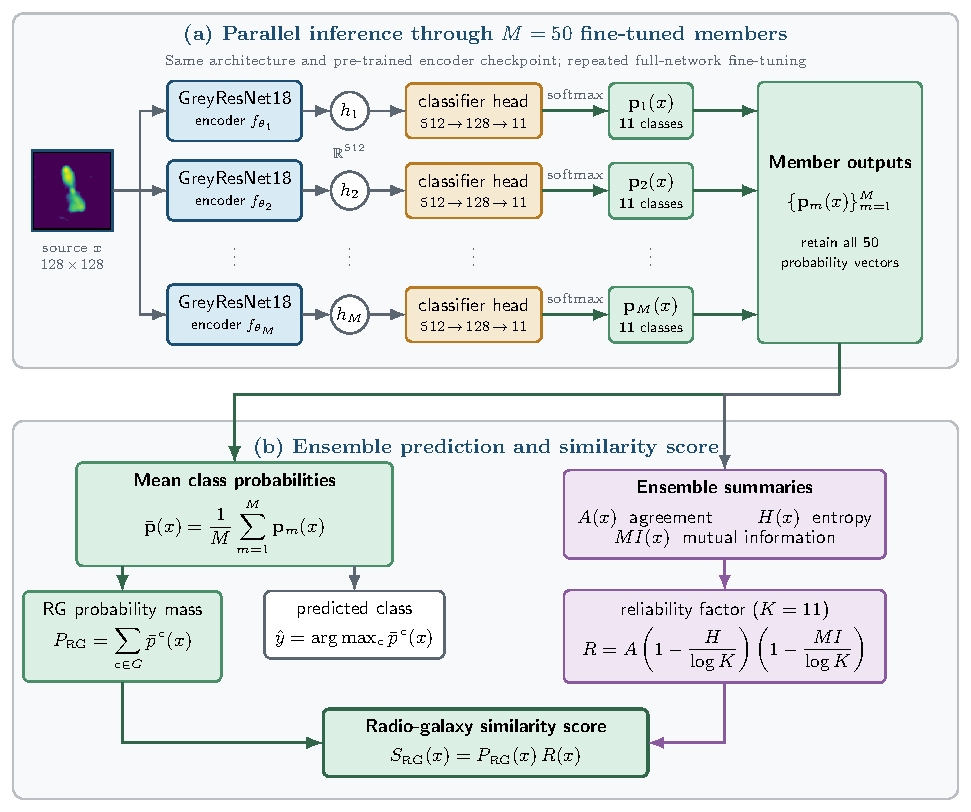
\includegraphics[width=\linewidth]{img/deep_ensemble_schematic.pdf}
  \caption[Deep-ensemble inference and similarity scoring]{Deep-ensemble inference and similarity scoring.}
  \label{fig:ensemble_schematic}
\end{figure}

\subsection{Similarity-to-radio-galaxy score \texorpdfstring{$S_\mathrm{RG}$}{S\_RG}}
\label{sec:method_srg}

Since the primary objective is not to reproduce a fixed external taxonomy but to quantify how strongly a source resembles the radio-galaxy morphologies represented by the model, we group the internal classes into \textit{radio-galaxy-like} (\(G\)) and \textit{non-target} (\(N\)) sets.

Using the internal model labels, the radio-galaxy-like set is defined as
\[
\begin{aligned}
G=\{&\text{Asymmetric core-jet (ACJ)},\\
	&\text{Bright-core},\\
	&\text{Centre-bright (FRI)},\\
	&\text{Core-Displaced},\\
	&\text{Edge-bright (FRII) linear},\\
	&\text{Hybrid (FRX) unclear},\\
	&\text{Large FRII},\\
	&\text{Structured-Bent}\},
\end{aligned}
\]
and the complementary set is
\[
N=\{\text{Amorphous},\ \text{Spirals},\ \text{Unresolved}\}.
\]

We define these groups operationally from the chosen visual classes, including core-dominated appearances in \(G\). Visual inspection of the optical overlays showed that the majority of the sources in the Spirals class are disc galaxies that exhibit radio emission associated with the galactic disc. Amorphous sources lack sufficiently distinct structure for this target, and Unresolved sources provide insufficient spatial information; either class may still contain physical radio galaxies.
This grouping leads to the definition of the radio-galaxy probability mass \(P_\mathrm{RG}\).
With \(\mathbf{p}_m(x)\) denoting the probability vector predicted for source \(x\) by ensemble member \(m\), as introduced in Eq.~\ref{eq:ensmean}, the radio-galaxy probability mass is
\begin{equation}
P_\mathrm{RG}(x)=\sum_{c\in G}\bar{p}^{\,c}(x), \qquad P_\mathrm{RG}(x)\in[0,1].
\label{eq:rg_prob_mass}
\end{equation}

This term measures only how much ensemble-mean probability is assigned to radio-galaxy-like classes.
It does not capture the concentration of the probability vector or the consistency of the member predictions.
Therefore, three complementary summaries -- model agreement \(A(x)\) (Eq.~\ref{eq:ensmean}), predictive entropy \(H(x)\) (Eq.~\ref{eq:H}), and mutual information \(MI(x)\) (Eq.~\ref{eq:MI}) -- are combined into the definition of a reliability factor, 
\begin{equation}
R(x)=A(x)\left(1-\frac{H(x)}{\log K}\right)\left(1-\frac{MI(x)}{\log K}\right).
\label{eq:reliab_factor}
\end{equation}

Dividing \(H\) and \(MI\) by \(\log K\) normalises them by their theoretical maxima for \(K\) classes.
All three factors, and therefore \(R\), lie in the range \([0,1]\).
Hence, the final \textit{similarity-to-radio-galaxy} score is
\begin{equation}
S_\mathrm{RG}(x)=P_\mathrm{RG}(x)\,R(x),\qquad S_\mathrm{RG}(x)\in[0,1].
\label{eq:sim_score}
\end{equation}
For a fixed model and preprocessing pipeline, the score is computed on the same \([0,1]\) scale for every source. Large \(S_\mathrm{RG}\) values indicate strong support for the chosen radio-galaxy-like model classes together with high ensemble consistency.

Fine-class ambiguity also reduces the score when all probability lies within \(G\). If every member assigns \(0.51\) to FRI and \(0.49\) to FRII, then \(P_\mathrm{RG}=A=1\) and \(MI=0\), but \(S_\mathrm{RG}\simeq0.711\). This design favours concentrated support for a particular learned morphology.

\begin{wraptable}{r}{0.40\textwidth}
\begin{minipage}{\linewidth}
\centering
\small
\setstretch{1}
\begin{tabular}{lrrr}
\toprule
 & \(A\) & \(H\) & \(MI\) \\
\midrule
\(A\)  & 1.00 & -0.62 & -0.52 \\
\(H\)  & -0.62 & 1.00 & 0.49 \\
\(MI\) & -0.52 & 0.49 & 1.00 \\
\bottomrule
\end{tabular}
\footnotesize
\caption[Correlations between ensemble reliability measures]{Empirical Pearson correlations between the reliability terms used in \(R(x)\), computed from the classified LoTSS-DR2 catalogue. }
\label{tab:reliability_corr}
\end{minipage}
\end{wraptable}
The reliability terms are empirically correlated (see Table~\ref{tab:reliability_corr}), but they summarise different aspects of the ensemble output. Agreement \(A\) uses only top-class votes, \(H\) measures how broadly the ensemble-mean probability is distributed across classes, and \(MI\) captures disagreement between the members’ probability distributions. Agreement tends to decrease as total or epistemic uncertainty increases, while \(H\) and \(MI\) increase together when ensemble predictions become less stable. Their multiplicative combination is a design choice.
\par
\ifnum\value{WF@wrappedlines}>1
  \vspace{\dimexpr\value{WF@wrappedlines}\baselineskip-\baselineskip\relax}
\fi
\WFclear

\subsection{External catalogue mapping and evaluation}
\label{sec:method_external_mapping}
\label{sec:bg_eval_metrics}

As we discussed in Sec.~\ref{sec:bg_taxonomy}, there is no single universally adopted taxonomy covering all of these morphologies. Therefore, we adopt the morphological correspondences in Table~\ref{tab:morph_mapping} for the comparisons in Sec.~\ref{sec:results_external}, rather than assuming exact equivalence between taxonomies.
In particular, one-sided ridgelines, X-shaped sources, winged sources, and relaxed doubles only approximately correspond to ACJ, Hybrid, Bent, and Amorphous, respectively.
We retain Clews et al.'s uncertain FRI and FRII labels within their respective groups. For external comparison, we combine Edge-bright FRII and Large FRII into a single FRII group.

Clews's one-sided ridgelines are an imperfect ACJ stand-in: inspection of \(100\) examples suggested that only about \(60\,\%\) were genuinely one-sided sources \citep{Clews2025}.
Our ambiguous Hybrid class is also broader than a physical FRI/FRII hybrid or an X-shaped morphology. These mappings support comparisons of related appearances, not interchangeable physical labels.

For Horton's multi-label catalogue, we assign the first class satisfying its conditions in the order FRI, FRII, Spirals, Amorphous, Hybrid, ACJ, then Bent.
Sources satisfying none of these rules remain unmapped; multiple flags do not automatically imply exclusion.

\begin{table}[H]
\centering
\small
\setlength{\tabcolsep}{3pt}
\renewcommand{\arraystretch}{1.15}
\begin{tabular}{@{}p{0.055\linewidth}p{0.16\linewidth}p{0.245\linewidth}p{0.26\linewidth}p{0.22\linewidth}@{}}
\hline
\raggedright Class ID & Class name & \raggedright\citet{Clews2025} & \raggedright\citet{Horton2025} & \citet{Chilufya2025}\\
\hline
0 & Amorphous & -- & \texttt{relaxed}$^a$, \texttt{diffuse}$^a$ & relaxed \\ \hline
1 & ACJ & one\_sided\_ridge & \texttt{onesided} & -- \\ \hline
2 & Bright-core & -- & -- & -- \\ \hline
3 & FRI & FRI, uncertain\_FRI & \texttt{fri}$^b$ & FRI \\ \hline
4 & Core-Displaced & -- & -- & -- \\ \hline
5 & FRII & FRII, uncertain\_FRII & \texttt{frii}$^b$ & FRII \\ \hline
6 & Hybrid & -- & \texttt{hybrid}, \texttt{xshaped} & -- \\ \hline
7 & Large FRII & -- & -- & -- \\ \hline
8 & Spirals & -- & \texttt{spiral} & -- \\ \hline
9 & Bent & bent & \raggedright \texttt{cshaped}$^a$, \texttt{sshaped}$^a$, \texttt{wings}$^a$ & WAT, NAT, headtail \\ \hline
10 & Unresolved & -- & -- & -- \\
\hline
\multicolumn{5}{@{}p{\linewidth}@{}}{Unmapped: Clews -- \textit{other}, \textit{triple}; Horton -- no mapping rule satisfied.} \\
\hline
\multicolumn{5}{@{}p{\linewidth}@{}}{\footnotesize $^a$ Only when \texttt{fri} and \texttt{frii} are both false.} \\
\multicolumn{5}{@{}p{\linewidth}@{}}{\footnotesize $^b$ Only when the other FR flag is false (exclusive).} \\
\end{tabular}
\caption[Mapping between external and internal morphology classes]{Adopted morphological correspondences between reference catalogues and our internal classes.
A dash (--) indicates that no direct mapping is adopted.}
\label{tab:morph_mapping}
\end{table}

For each external-catalogue comparison, the target morphology defines the positive class and the remaining mapped morphologies define the negative class.
A true positive (\(\mathrm{TP}\)) or true negative (\(\mathrm{TN}\)) agrees with the reference assignment. 
A false positive (\(\mathrm{FP}\)) is predicted positive but is negative in the reference, while a false negative (\(\mathrm{FN}\)) is predicted negative but is positive in the reference.
These four counts form the confusion matrix. Precision measures the purity of the predicted positive sample, whereas recall measures the completeness of the positive class:
\begin{equation}
\mathrm{precision}=\frac{\mathrm{TP}}{\mathrm{TP}+\mathrm{FP}},\qquad
\mathrm{recall}=\frac{\mathrm{TP}}{\mathrm{TP}+\mathrm{FN}}.
\end{equation}
The \(F_1\) score combines precision and recall through their harmonic mean,
\begin{equation}
F_1=2\,\frac{\mathrm{precision}\,\mathrm{recall}}{\mathrm{precision}+\mathrm{recall}}.
\end{equation}

A higher \(F_1\) score indicates better classification performance on the evaluated sample.

We estimate uncertainty in the reported metrics from the number of evaluated sources and repeated resampling of each comparison sample. The resulting bounds describe how the metrics may vary with sample membership -- label errors, selection bias and training variability require separate assessment.
Each catalogue is evaluated separately, with calculation details in Appendix~\ref{app:evaluation}.

We also repeat the comparisons after excluding all \(2\,657\) curated sources, across angular-size ranges, and without Clews's uncertain FR labels. Excluding curated sources removes overlap with supervised training, although the remaining sources still participated in pre-training.

\subsection{Application to diffuse radio emission}
\label{sec:method_relics}

We used the selected radio relics described in Sec.~\ref{sec:data_relics} to test the trained ensemble on diffuse radio emission.
The aim is to examine how their morphology is represented by the radio-galaxy classifier. 
Bright radio galaxies within a relic cutout can dominate the normalised input, while clipping can suppress the relic's low-surface-brightness emission.
We therefore mask neighbouring sources before preprocessing to focus the test on the diffuse emission.

We start with relic-centred LoTSS-DR3 cutouts with a side length of \(1.5\times\mathrm{LAS}\). Then, we manually draw polygonal regions around the relic emission, exclude pixels outside them, estimate the sigma-clipped standard deviation \(\sigma\) from the retained pixels and then set both masked pixels and values below \(3\sigma\) to this floor. The images are resampled to \(128\times128\) pixels and min--max normalised for inference.

These selected examples illustrate the model's response to isolated relic emission, rather than its performance on unmasked fields. The assigned labels describe resemblance to the learned classes.


\cleartooddpage
\section{Results}
\label{sec:results}

In this chapter we present the morphology catalogue and similarity scores produced by the trained ensemble. First, the internal class assignments and score distributions are described; then we compare the predictions with external morphology catalogues. Finally, we examine the model response to selected radio relics.

\subsection{Internal classification and \texorpdfstring{$S_\mathrm{RG}$}{S\_RG} evaluation}
\label{sec:results_internal}

The internal results summarise the ensemble predictions across the full LoTSS-DR2 sample. Class membership, confidence and agreement are presented first, followed by the distributions of the similarity-score components and membership in the adopted score bands.

\subsubsection{Ensemble classification catalogue}
\label{sec:results_classification}

The ensemble classification catalogue contains \(32\,514\) sources across eleven morphology classes (Table~\ref{tab:classification_catalogue}). Edge-bright FRII and Structured-Bent are the most common assignments, together accounting for \(45.4\,\%\) of the sample, whereas Amorphous sources constitute only \(1.2\,\%\). These are predicted image-morphology groups, rather than independently confirmed physical source populations.

Bright-core sources have the highest mean confidence, while Amorphous and Asymmetric core-jet sources have the lowest (Table~\ref{tab:classification_catalogue}). Confidence and agreement describe the concentration and consistency of predictions, rather than classification accuracy. Figure~\ref{fig:classification_confidence_extremes} compares the most and least confident assignments within each class.

The ensemble correctly classifies \(28\) of the \(33\) test images withheld from supervised training (\(84.8\,\%\)). Most errors involve ACJ and Structured-Bent sources (Table~\ref{tab:heldout_counts}). With only three examples per class and prior exposure during pre-training, this test provides limited evidence of performance on new survey sources.

\begin{table}[H]
\centering
\small
\begin{tabular}{lrrrr}
\toprule
Class & Count & Fraction & Confidence & Agreement \\
\midrule
Amorphous & 390 & 1.2\,\% & 0.651 & 0.869 \\
Asymmetric core-jet (ACJ) & 1\,976 & 6.1\,\% & 0.660 & 0.894 \\
Bright-core & 3\,728 & 11.5\,\% & 0.865 & 0.946 \\
Centre-bright (FRI) & 3\,323 & 10.2\,\% & 0.785 & 0.912 \\
Core-Displaced & 980 & 3.0\,\% & 0.697 & 0.834 \\
Edge-bright (FRII) linear & 7\,574 & 23.3\,\% & 0.821 & 0.931 \\
Hybrid (FRX) unclear & 2\,865 & 8.8\,\% & 0.718 & 0.909 \\
Large FRII & 2\,425 & 7.5\,\% & 0.774 & 0.876 \\
Spirals & 963 & 3.0\,\% & 0.756 & 0.907 \\
Structured-Bent & 7\,197 & 22.1\,\% & 0.740 & 0.918 \\
Unresolved & 1\,093 & 3.4\,\% & 0.711 & 0.873 \\
\midrule
Total & 32\,514 & 100\,\% & & \\
\bottomrule
\end{tabular}
\caption[Class composition, confidence and agreement]{Class composition and mean ensemble confidence and agreement.}
\label{tab:classification_catalogue}
\end{table}

\begin{figure}[H]
\centering
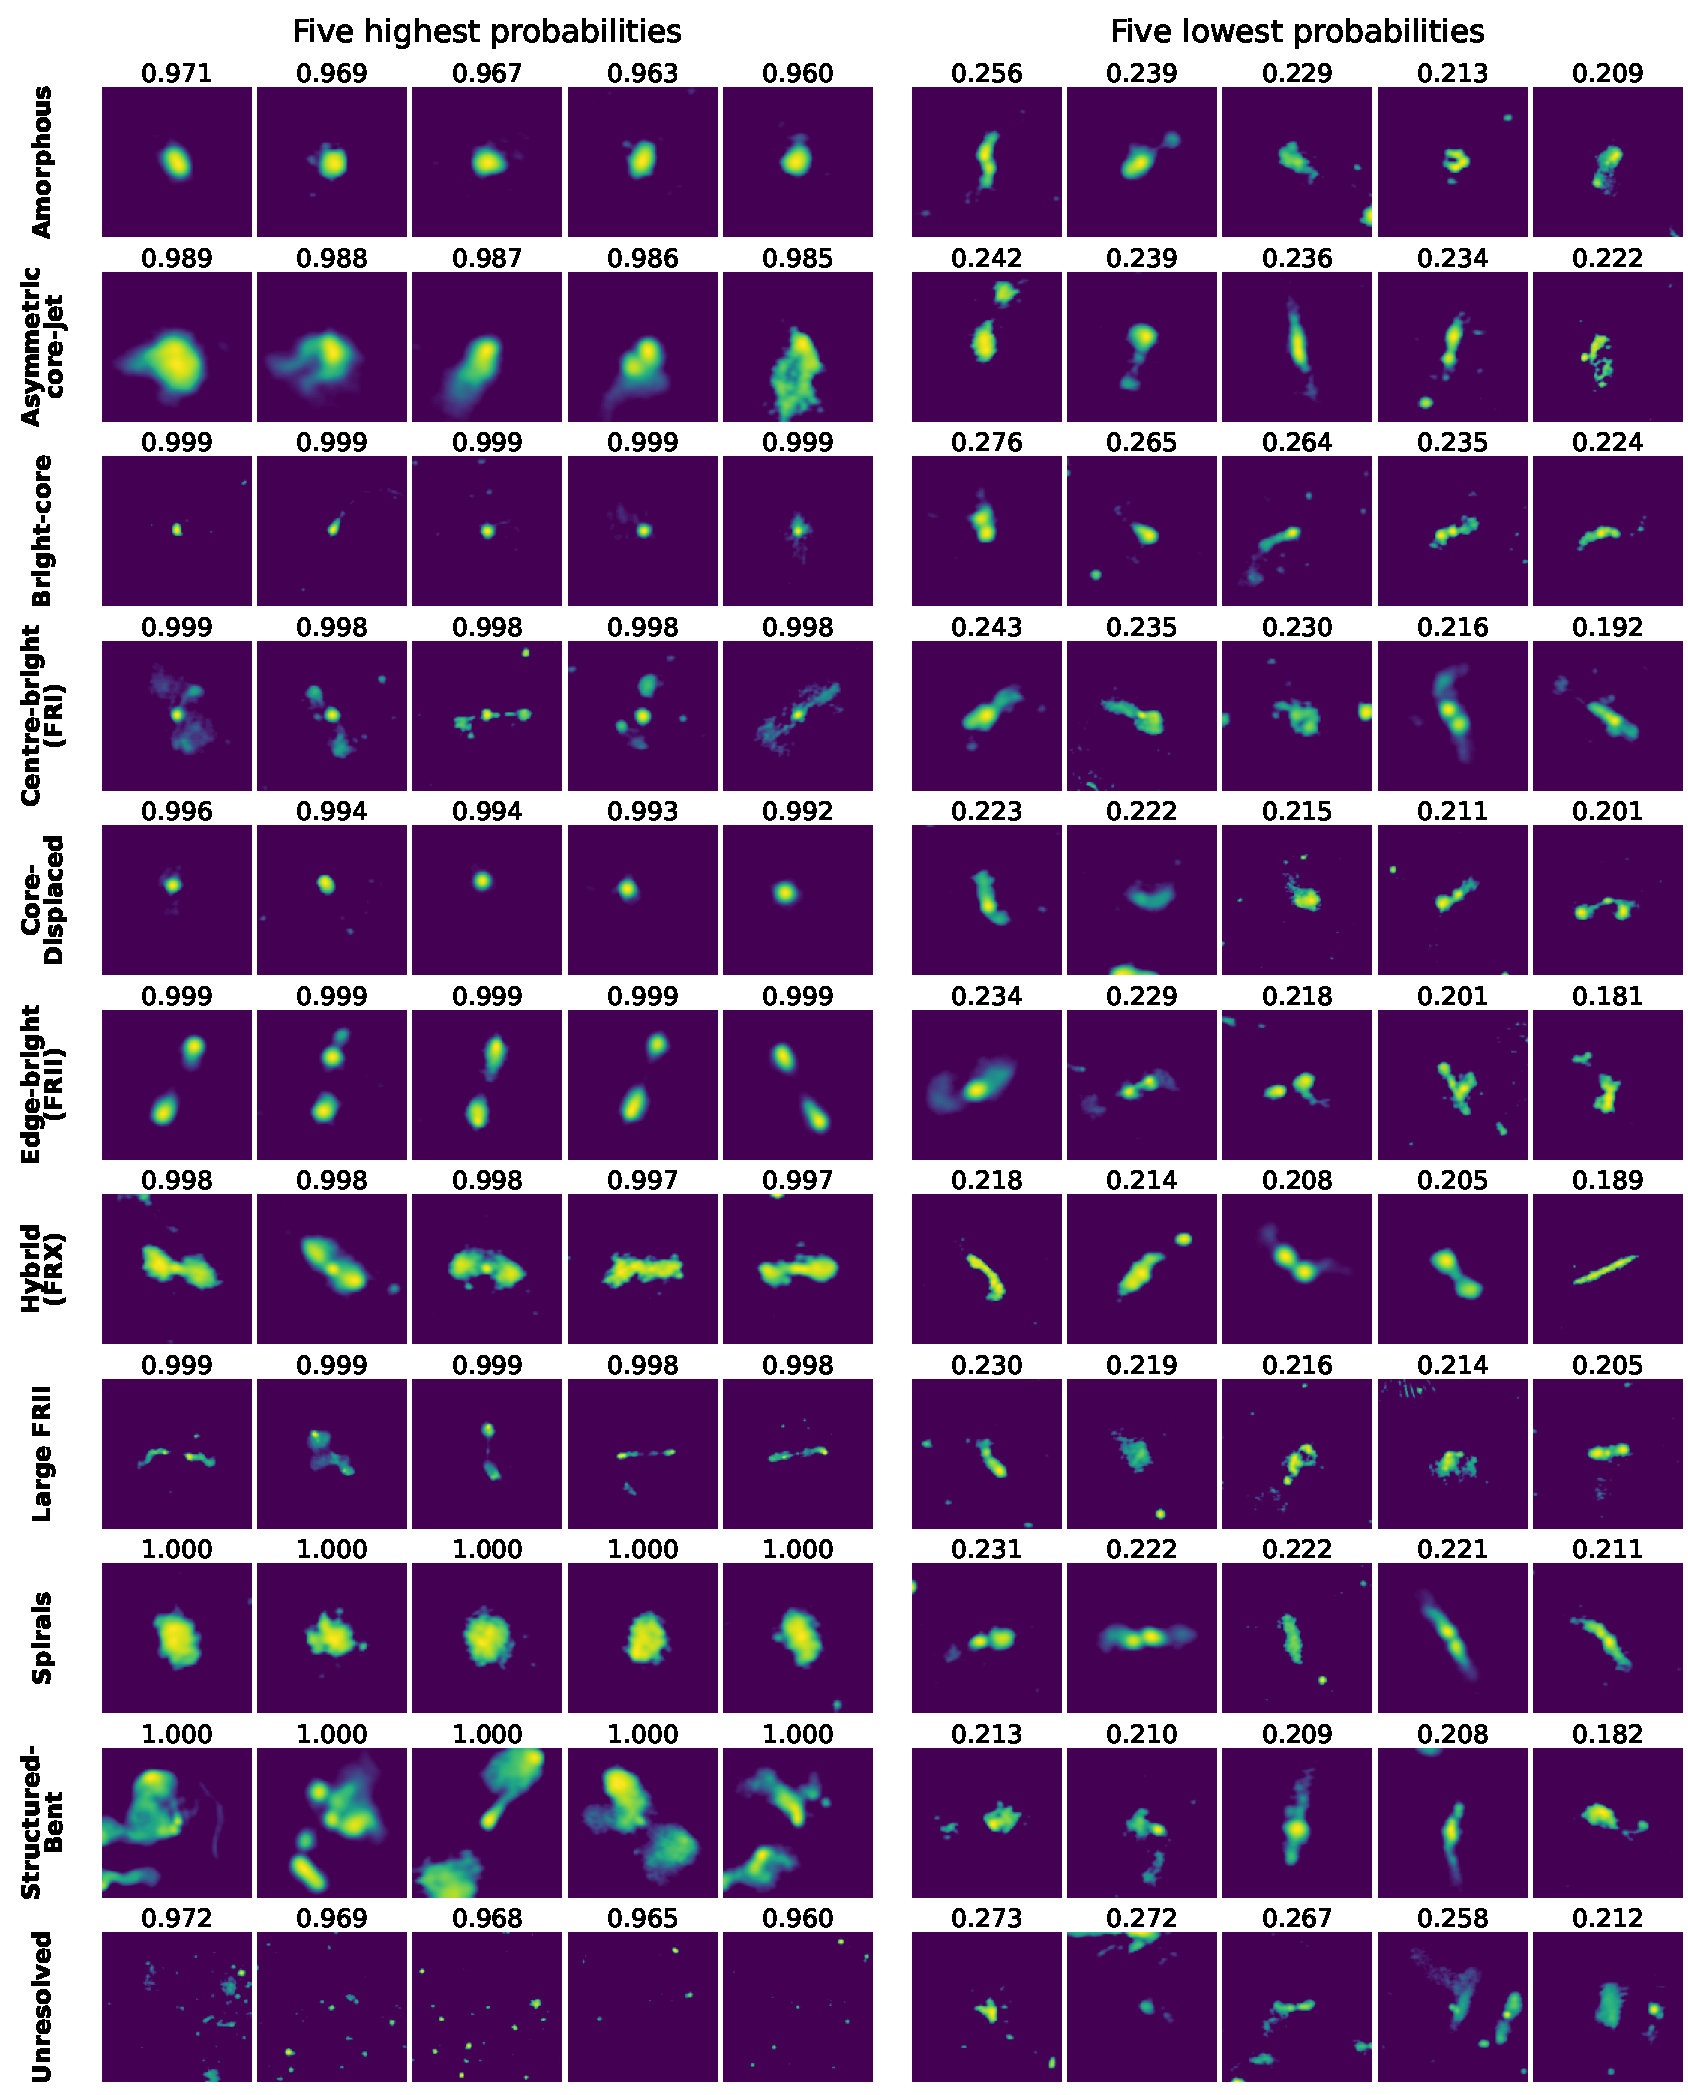
\includegraphics[width=\linewidth]{img/classification_confidence_extremes.pdf}
\caption[Highest- and lowest-confidence examples by class]{Five highest-confidence (left) and five lowest-confidence (right) sources per predicted class. Values above cutouts are ensemble-mean probabilities of the assigned class.}
\label{fig:classification_confidence_extremes}
\end{figure}
\clearpage

\subsubsection{Score distributions and operational bands}

Figure~\ref{fig:srg_dist} shows how the class probabilities and ensemble consistency combine into \(S_\mathrm{RG}\). The radio-galaxy probability mass \(P_\mathrm{RG}\) is concentrated near unity, while the reliability factor \(R\) is more broadly distributed. A large probability mass in the radio-galaxy-like classes therefore does not necessarily produce a high final score.

\begin{figure}[H]
\centering
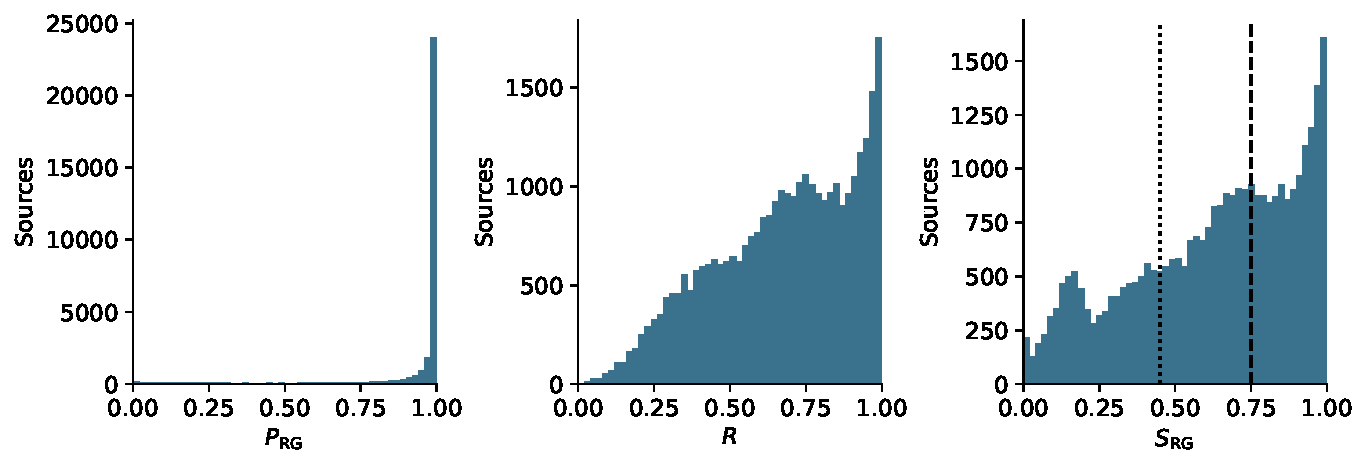
\includegraphics[width=\linewidth]{img/srg_distributions.pdf}
\caption[Full-catalogue score distributions]{Score components for all \(32\,514\) sources. The dashed and dotted lines in the right panel mark \(S_\mathrm{RG}=0.75\) and \(0.45\), respectively.}
\label{fig:srg_dist}
\end{figure}

Table~\ref{tab:srg_bands} divides the catalogue into the adopted high, transitional and low similarity bands. The high-score band is the largest of these review subsets.

\begin{table}[H]
\centering
\begin{tabular}{lrr}
\toprule
Band & Count & Fraction \\
\midrule
High: \(S_\mathrm{RG}\geq0.75\) & 12\,875 & 39.6\,\% \\
Transitional: \(0.45\leq S_\mathrm{RG}<0.75\) & 10\,956 & 33.7\,\% \\
Low: \(S_\mathrm{RG}<0.45\) & 8\,683 & 26.7\,\% \\
\bottomrule
\end{tabular}
\caption[Catalogue membership by score band]{Catalogue membership in the three operational score bands.}
\label{tab:srg_bands}
\end{table}

The class-conditioned distributions in Figure~\ref{fig:srg_class} reflect both the adopted \(G/N\) grouping and the ensemble's support for individual predictions. The non-target classes favour low scores; within \(G\), Bright-core has the highest median and Core-Displaced the lowest. The substantial spread within classes shows why a class assignment alone does not determine the review band.

\begin{figure}[H]
\centering
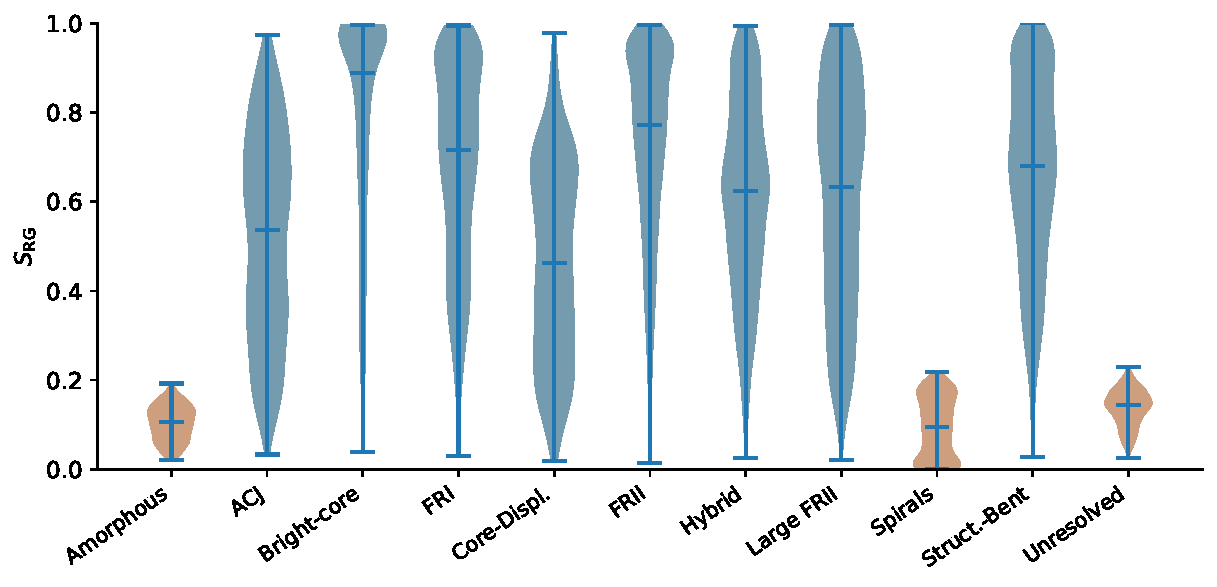
\includegraphics[width=\linewidth]{img/srg_per_class.pdf}
\caption[Similarity-score distributions by predicted class]{Score distributions by ensemble-assigned class. Blue and orange denote the \(G\) and \(N\) groups; central horizontal marks show medians.}
\label{fig:srg_class}
\end{figure}


\subsection{Comparison with external morphology catalogues}
\label{sec:results_external}

We compare the ensemble assignments with the mapped labels of \citet{Clews2025}, \citet{Horton2025}, and \citet{Chilufya2025}, using the correspondences in Sec.~\ref{sec:method_external_mapping}. The mapped samples in Table~\ref{tab:external_individual_samples} include \(645\), \(718\), and \(198\) members of the internally curated subsample, respectively. These comparisons assess agreement with independently compiled label schemes, not an established physical ground truth. FRII includes both Edge-bright FRII and Large FRII throughout the comparison.

The main findings remain after excluding all curated sources (Table~\ref{tab:excluded_curated}). The figures retain the full mapped samples; Appendix~\ref{app:evaluation} gives additional checks. The exclusion removes overlap with supervised training, although these sources still participated in pre-training.
This check uses the curated-excluded selections in the final column of Table~\ref{tab:external_individual_samples}.

\begin{table}[H]
\centering
\small
\setstretch{1}
\setlength{\tabcolsep}{8pt}
\renewcommand{\arraystretch}{1.6}
\begin{tabular}{@{}lrrr@{}}
\toprule
Catalogue & Sources & FRI \(F_1\) & FRII \(F_1\) \\
\midrule
Clews & 7757 & \(0.389_{-0.021}^{+0.020}\) & \(0.735_{-0.013}^{+0.013}\) \\
Horton & 8352 & \(0.281_{-0.022}^{+0.020}\) & \(0.743_{-0.010}^{+0.010}\) \\
Chilufya & 2590 & \(0.445_{-0.036}^{+0.036}\) & \(0.455_{-0.033}^{+0.032}\) \\
\bottomrule
\end{tabular}

\caption[External correspondence excluding curated sources]{External correspondence after excluding all curated sources. Signed uncertainties give the distances to the \(95\,\%\) interval bounds.}
\label{tab:excluded_curated}
\end{table}

Figure~\ref{fig:ext_confusion_fri} shows the class correspondence for all three catalogues. We then examine FRI and FRII separately.

\begin{figure}[H]
\centering
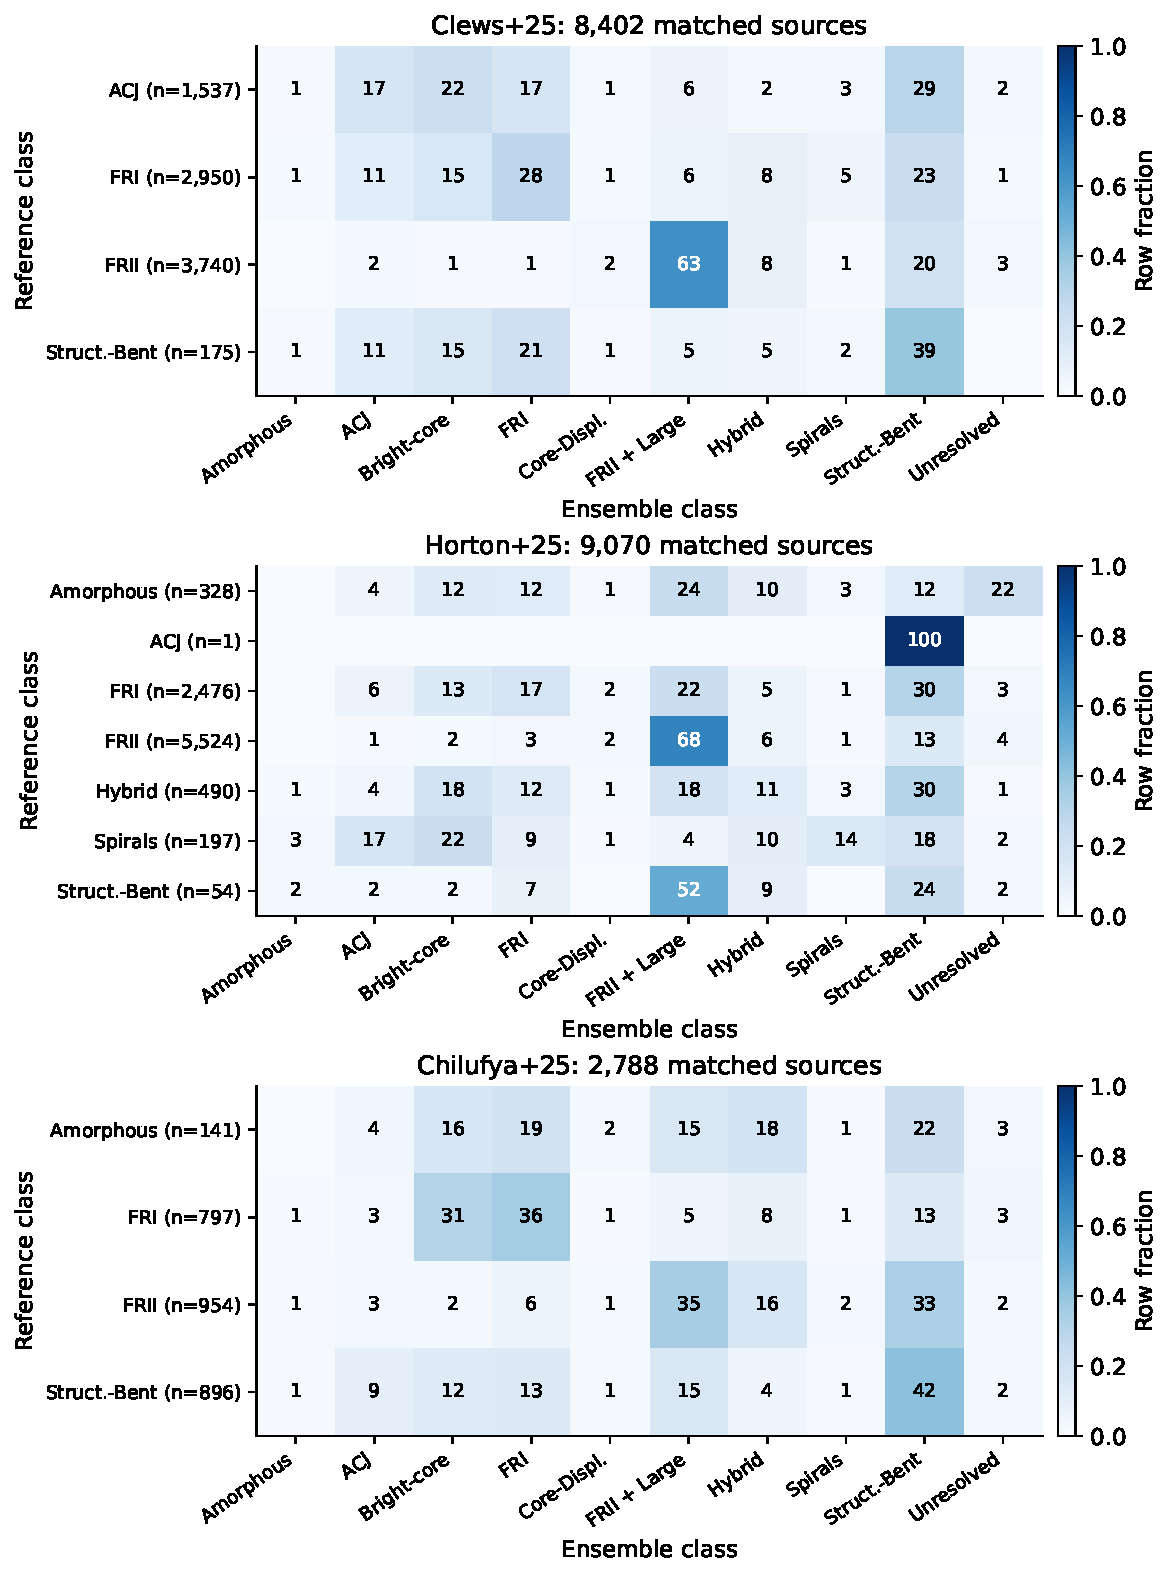
\includegraphics[width=\linewidth,height=0.87\textheight,keepaspectratio]{img/ext_confusion_FRII-relaxed.pdf}
\caption[Class correspondence with external catalogues]{Row-normalised class correspondence for Clews, Horton, and Chilufya. Rows are reference classes with source counts in parentheses; columns are ensemble predictions. Edge-bright FRII and Large FRII predictions are combined. Cells above \(0.5\,\%\) are annotated with percentages; reference classes absent from a catalogue are omitted.}
\label{fig:ext_confusion_fri}
\label{fig:ext_confusion_frii_r}
\end{figure}

\subsubsection{FRI correspondence}
\label{sec:ext_fri}

The model recovers FRI morphology poorly across all three catalogues (Table~\ref{tab:ext_fri}).

\begin{table}[H]
\centering
\small
\setlength{\tabcolsep}{4pt}
\setstretch{1}
\renewcommand{\arraystretch}{1.6}
\begin{tabular}{@{}lrrrrr@{}}
\toprule
Catalogue & Reference sources & TP & FP & FN & \(F_1\) \\
\midrule
Clews & 2950 & 818 & 334 & 2132 & \(0.399_{-0.019}^{+0.019}\) \\
Horton & 2476 & 431 & 278 & 2045 & \(0.271_{-0.020}^{+0.020}\) \\
Chilufya & 797 & 285 & 198 & 512 & \(0.445_{-0.035}^{+0.033}\) \\
\bottomrule
\end{tabular}

\caption[FRI agreement with external catalogues]{FRI agreement with the mapped reference labels; uncertainties indicate \(95\,\%\) intervals.}
\label{tab:ext_fri}
\end{table}

Frequent Bright-core assignments suggest that central brightness dominates over extended jets and lobes, while Structured-Bent assignments reveal sensitivity to bending (Figure~\ref{fig:ext_fn_fri}). These patterns also reflect catalogue-dependent class boundaries, particularly Horton's inclusion of curved sources within FRI \citep{Horton2025}.

\begin{figure}[H]
\centering
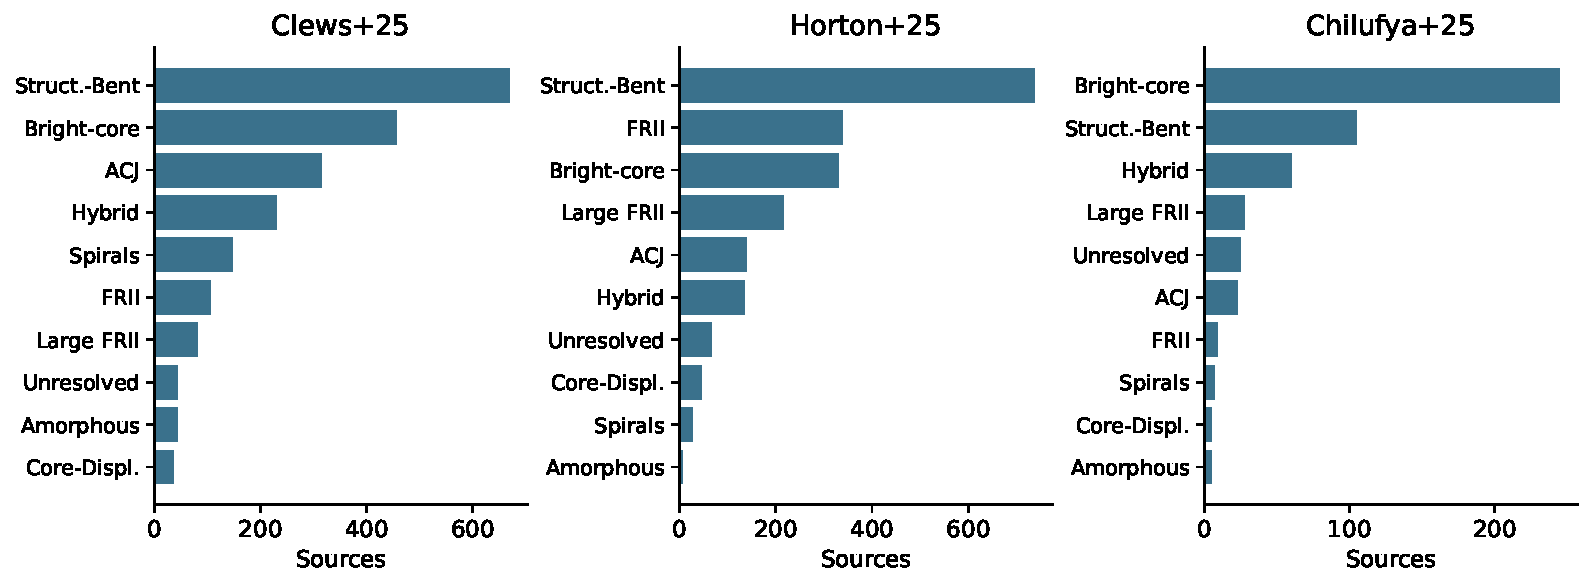
\includegraphics[width=\linewidth]{img/ext_fn_breakdown_FRI.pdf}
\caption[Predicted classes of missed reference FRI sources]{Ensemble assignments of reference FRI sources not predicted as FRI.}
\label{fig:ext_fn_fri}
\end{figure}

The ensemble also assigns alternative morphologies to reference FRI sources with high confidence (Figure~\ref{fig:ext_conf_fri}).

\begin{figure}[H]
\centering
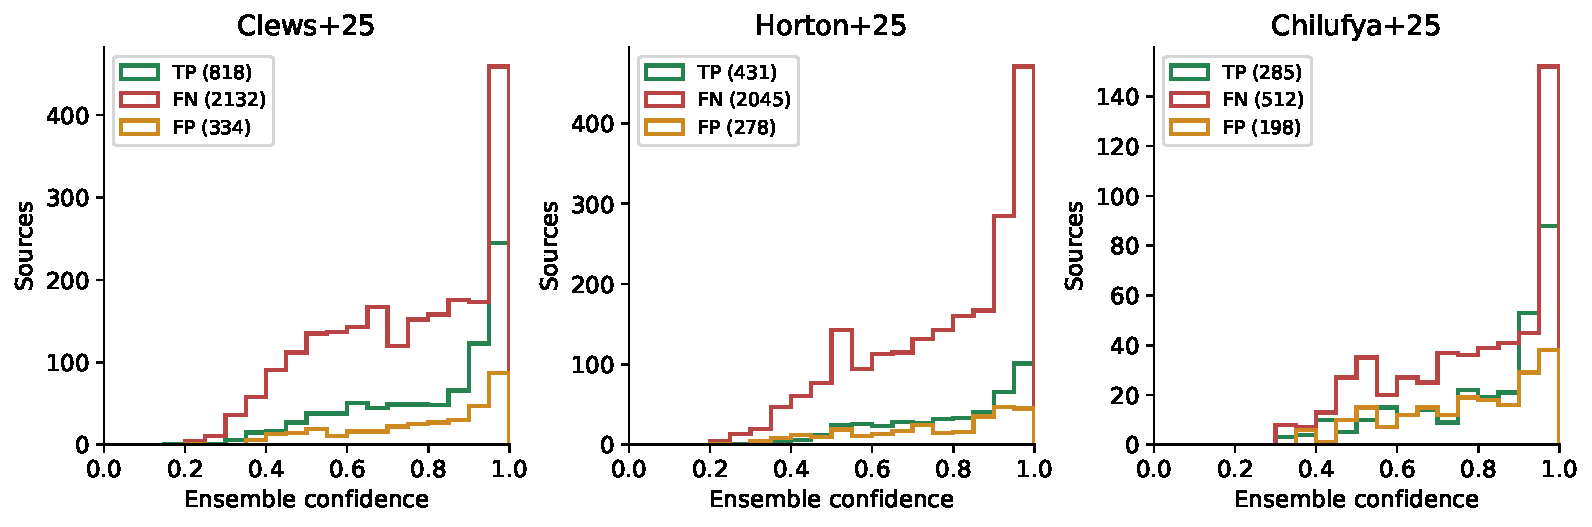
\includegraphics[width=\linewidth]{img/ext_confidence_FRI.pdf}
\caption[Ensemble confidence in the FRI comparisons]{Ensemble confidence for FRI true positives, false negatives, and false positives relative to each reference catalogue.}
\label{fig:ext_conf_fri}
\end{figure}

\subsubsection{FRII correspondence}
\label{sec:ext_frii}

FRII correspondence is strongest against Clews and Horton and weaker against Chilufya (Table~\ref{tab:ext_frii}).

\begin{table}[H]
\centering
\small
\setlength{\tabcolsep}{4pt}
\setstretch{1}
\renewcommand{\arraystretch}{1.6}
\begin{tabular}{@{}lrrrrr@{}}
\toprule
Catalogue & Reference sources & TP & FP & FN & \(F_1\) \\
\midrule
Clews & 3740 & 2359 & 287 & 1381 & \(0.739_{-0.012}^{+0.012}\) \\
Horton & 5524 & 3744 & 759 & 1780 & \(0.747_{-0.010}^{+0.010}\) \\
Chilufya & 954 & 333 & 192 & 621 & \(0.450_{-0.032}^{+0.032}\) \\
\bottomrule
\end{tabular}

\caption[FRII agreement with external catalogues]{FRII agreement with the mapped reference labels; uncertainties indicate \(95\,\%\) intervals.}
\label{tab:ext_frii}
\end{table}

Against Chilufya, FRI and FRII performance is similar, including after curated-source exclusion.

The remaining disagreements concentrate in Structured-Bent and Hybrid across all three catalogues (Figure~\ref{fig:ext_fn_frii}). This pattern suggests that curvature and mixed brightening patterns complicate the model's recognition of edge-brightened FRII structure.

\begin{figure}[H]
\centering
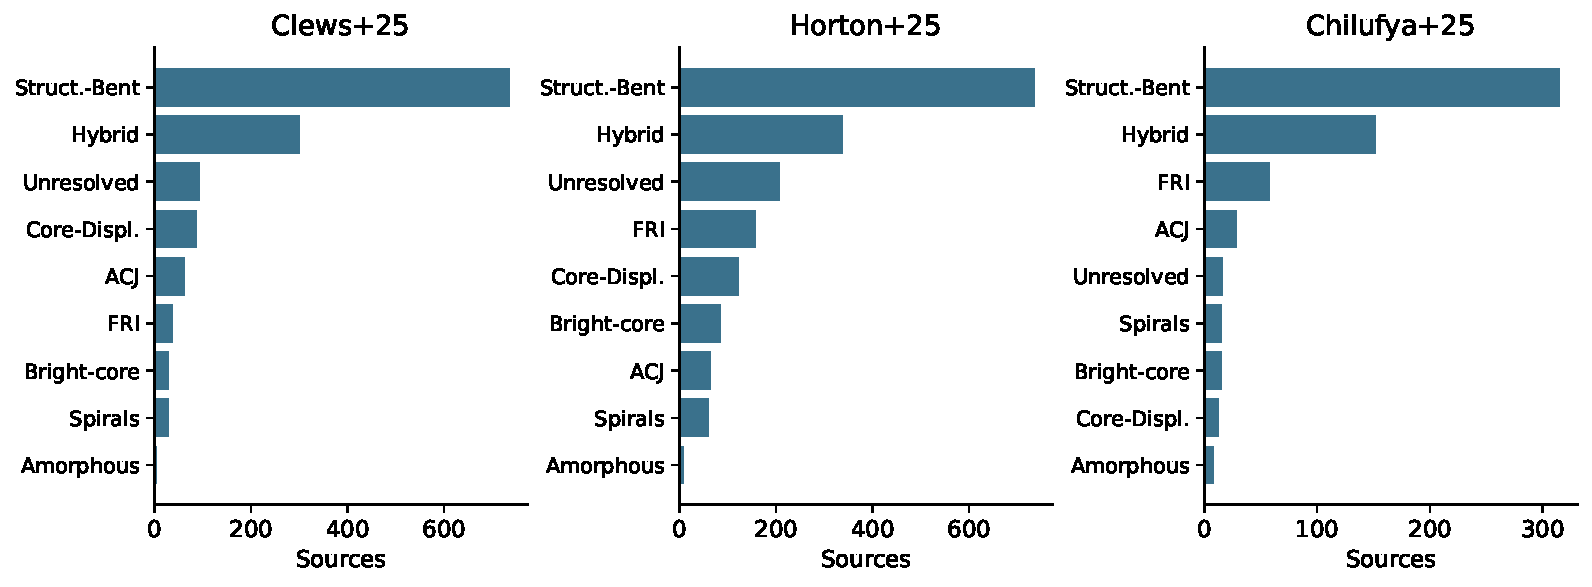
\includegraphics[width=\linewidth]{img/ext_fn_breakdown_FRII-relaxed.pdf}
\caption[Predicted classes of missed reference FRII sources]{Ensemble assignments of reference FRII sources predicted as neither Edge-bright FRII nor Large FRII.}
\label{fig:ext_fn_frii}
\end{figure}

Reference FRII sources assigned to either internal FRII class have higher median confidence than those assigned to other classes (Figure~\ref{fig:ext_conf_frii}).

\begin{figure}[H]
\centering
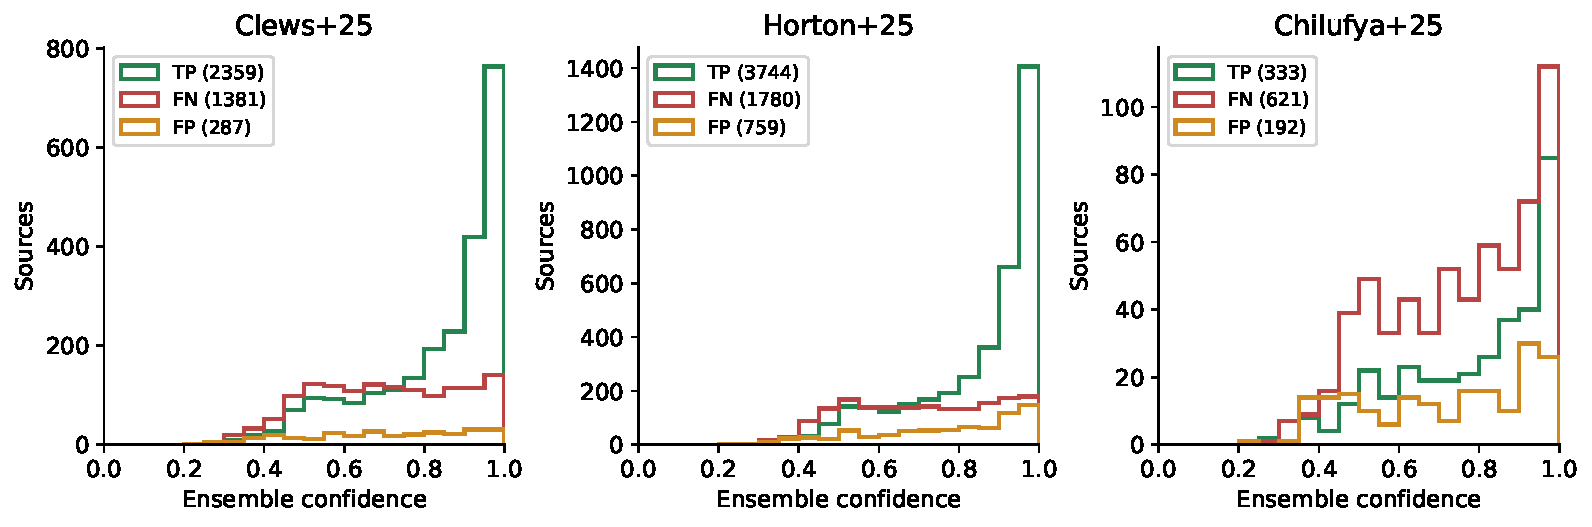
\includegraphics[width=\linewidth]{img/ext_confidence_FRII-relaxed.pdf}
\caption[Ensemble confidence in the FRII comparisons]{Ensemble confidence for FRII true positives, false negatives, and false positives.}
\label{fig:ext_conf_frii}
\end{figure}

\subsubsection{Three-catalogue consensus}
\label{sec:ext_consensus}

Of the sources in the common-source sample defined in Table~\ref{tab:external_combined_samples}, \(311\) have usable mapped labels in all three references. Of these, \(149\) receive the same mapped label, forming the consensus subset independently of the ensemble predictions; ten belong to the curated subsample. The ensemble agrees with the common reference label for fewer than half of these sources (Table~\ref{tab:ext_consensus}).

\begin{table}[H]
\centering
\small
\setlength{\tabcolsep}{5pt}
\setstretch{1}
\renewcommand{\arraystretch}{1.6}
\begin{tabular}{@{}lrrrrr@{}}
\toprule
Reference class & Sources & TP & FP & FN & \(F_1\) \\
\midrule
FRI & 62 & 25 & 0 & 37 & \(0.575_{-0.136}^{+0.117}\) \\
FRII & 87 & 43 & 4 & 44 & \(0.642_{-0.104}^{+0.090}\) \\
\bottomrule
\end{tabular}

\caption[Agreement with three-catalogue consensus labels]{Agreement with labels shared by all three catalogues; uncertainties indicate \(95\,\%\) intervals.}
\label{tab:ext_consensus}
\end{table}

Agreement remains below half after excluding the curated sources.
Reference FRI sources receive Bright-core assignments almost as often as FRI assignments, while reference FRII disagreements mainly involve Structured-Bent and Hybrid (Figure~\ref{fig:ext_consensus}).
\begin{figure}[H]
\centering
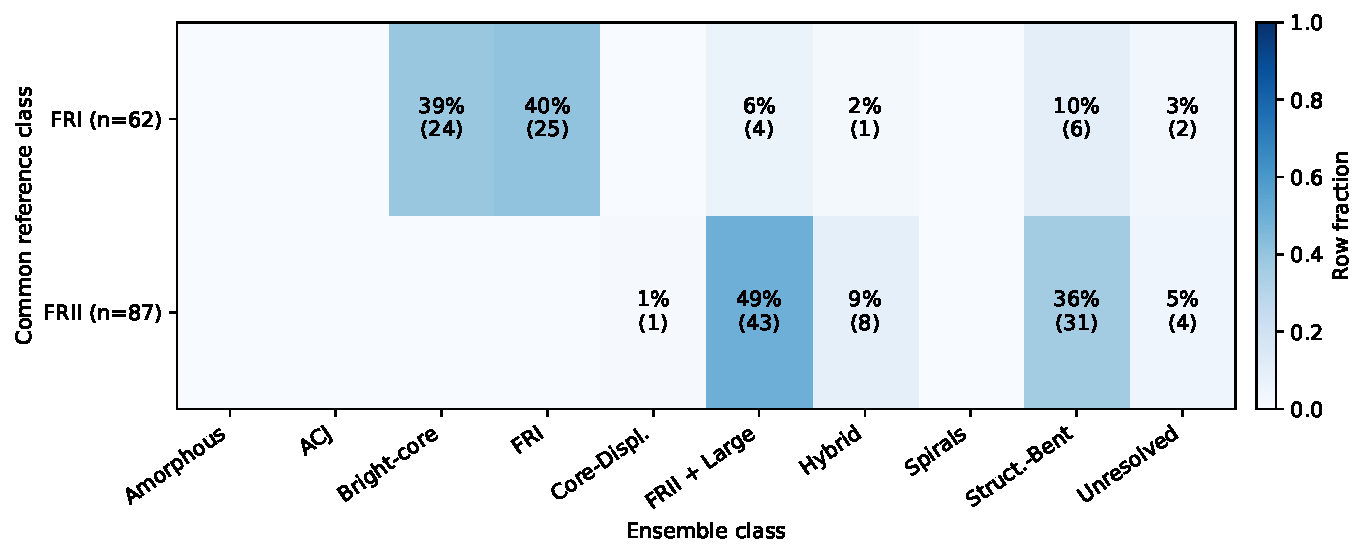
\includegraphics[width=0.8\linewidth]{img/ext_confusion_consensus.pdf}
\caption[Predicted classes of three-catalogue consensus sources]{Ensemble assignments for the \(149\) three-catalogue consensus sources. Cells give row percentages and source counts.}
\label{fig:ext_consensus}
\end{figure}

\subsubsection{\texorpdfstring{\(S_\mathrm{RG}\)}{S\_RG} distribution across mapped-reference sources}
\label{sec:ext_group_retention}
\label{sec:ext_gallery}
\label{sec:ext_summary}

Table~\ref{tab:ext_group_retention} includes all sources with a usable reference label in either \(G\) or \(N\). For each catalogue, we separate fine-class agreements from disagreements and report the ensemble's \(G/N\) assignments within each subset.

\begin{table}[h]
\centering
\small
\setlength{\tabcolsep}{4pt}
\begin{tabular}{@{}llrrrr@{}}
\toprule
Catalogue & Subset & Sources & \shortstack[r]{Share\\(\%)} & \shortstack[r]{Assigned to \(G\)\\\(n\) (row \%)} & \shortstack[r]{Assigned to \(N\)\\\(n\) (row \%)} \\
\midrule
Clews & All mapped & 8\,402 & 100.0 & 7\,943 (94.5) & 459 (5.5) \\
 & Agreements & 3\,501 & 41.7 & 3\,501 (100.0) & 0 (0.0) \\
 & Disagreements & 4\,901 & 58.3 & 4\,442 (90.6) & 459 (9.4) \\
\midrule
Horton & All mapped & 9\,070 & 100.0 & 8\,551 (94.3) & 519 (5.7) \\
 & Agreements & 4\,271 & 47.1 & 4\,244 (99.4) & 27 (0.6) \\
 & Disagreements & 4\,799 & 52.9 & 4\,307 (89.7) & 492 (10.3) \\
\midrule
Chilufya & All mapped & 2\,788 & 100.0 & 2\,670 (95.8) & 118 (4.2) \\
 & Agreements & 991 & 35.5 & 991 (100.0) & 0 (0.0) \\
 & Disagreements & 1\,797 & 64.5 & 1\,679 (93.4) & 118 (6.6) \\
\bottomrule
\end{tabular}
\caption[Group assignments for fine-class agreements and disagreements]{Fine-class correspondence for all mapped reference sources.}
\label{tab:ext_group_retention}
\end{table}

Figure~\ref{fig:ext_srg_distributions} shows the score components for the \(16\,177\) study sources with at least one mapped reference label (Table~\ref{tab:external_combined_samples}).
Each source is counted once, irrespective of catalogue overlap or agreement with the ensemble. 
For sources assigned to \(N\), the \(P_\mathrm{RG}\) distribution is concentrated towards low values, indicating weak support for radio-galaxy-like morphologies.
Their scores remain below \(S_\mathrm{RG}=0.25\), even where ensemble reliability is high.

\begin{figure}[H]
\centering
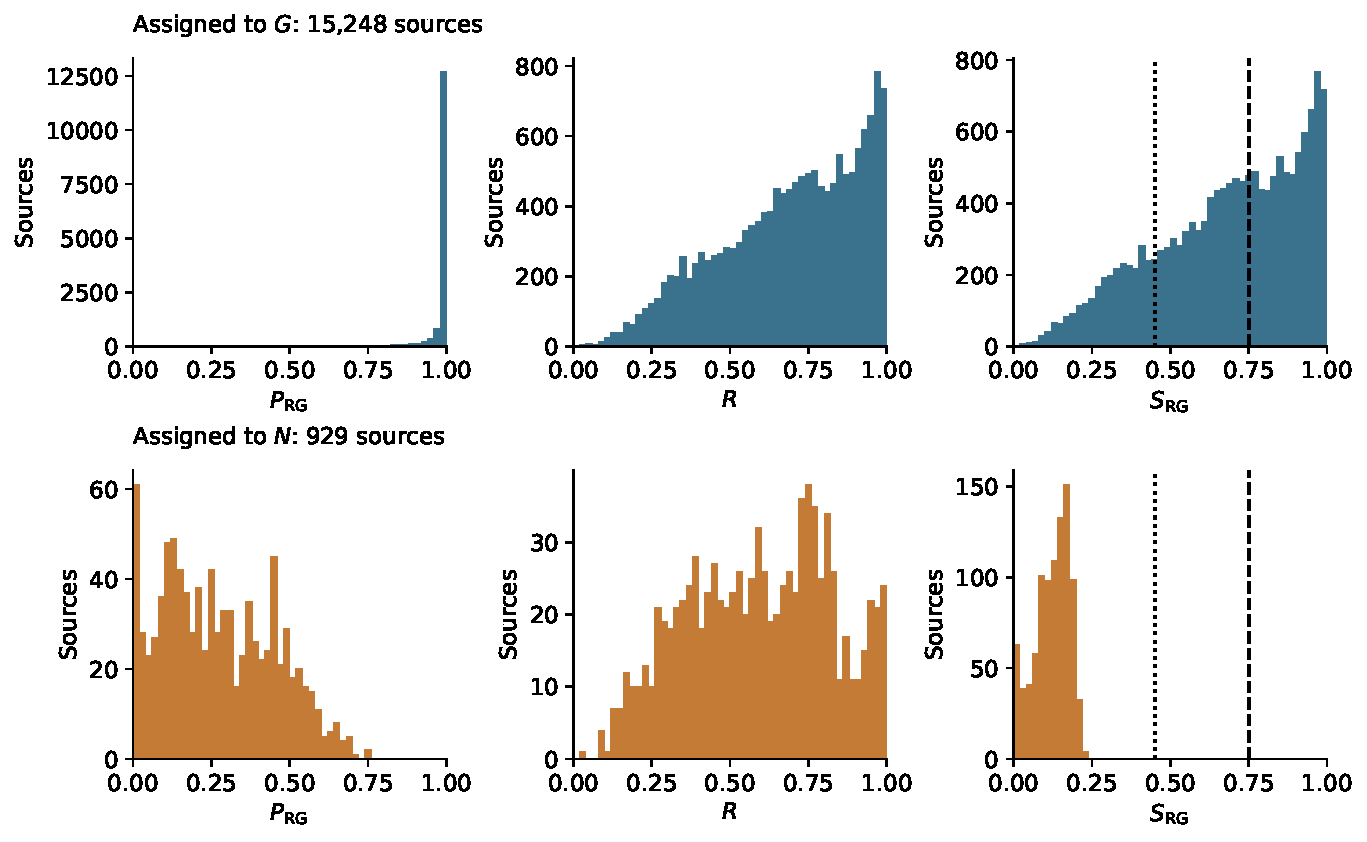
\includegraphics[width=\linewidth]{img/external_srg_distributions.pdf}
\caption[Score distributions for mapped-reference sources]{Score components for sources with mapped reference labels, separated by ensemble-assigned \(G\) (top) and \(N\) (bottom). Dashed and dotted lines mark \(S_\mathrm{RG}=0.75\) and \(0.45\).}
\label{fig:ext_srg_distributions}
\end{figure}

For the visual examples in Figure~\ref{fig:agree_gallery}, we select sources with at least one mapped reference label and agreement between every available mapped label and the ensemble assignment. We show five examples for each of six internal classes (ACJ, FRI, FRII, Hybrid, Spirals, and Structured-Bent).
We prioritise sources covered by more reference catalogues. These examples illustrate agreement without assuming its prevalence. In Appendix~\ref{app:external_disagreements} we present the complementary inspection sample (disagreement examples for each of the eleven internal classes).

\begin{figure}[H]
\centering
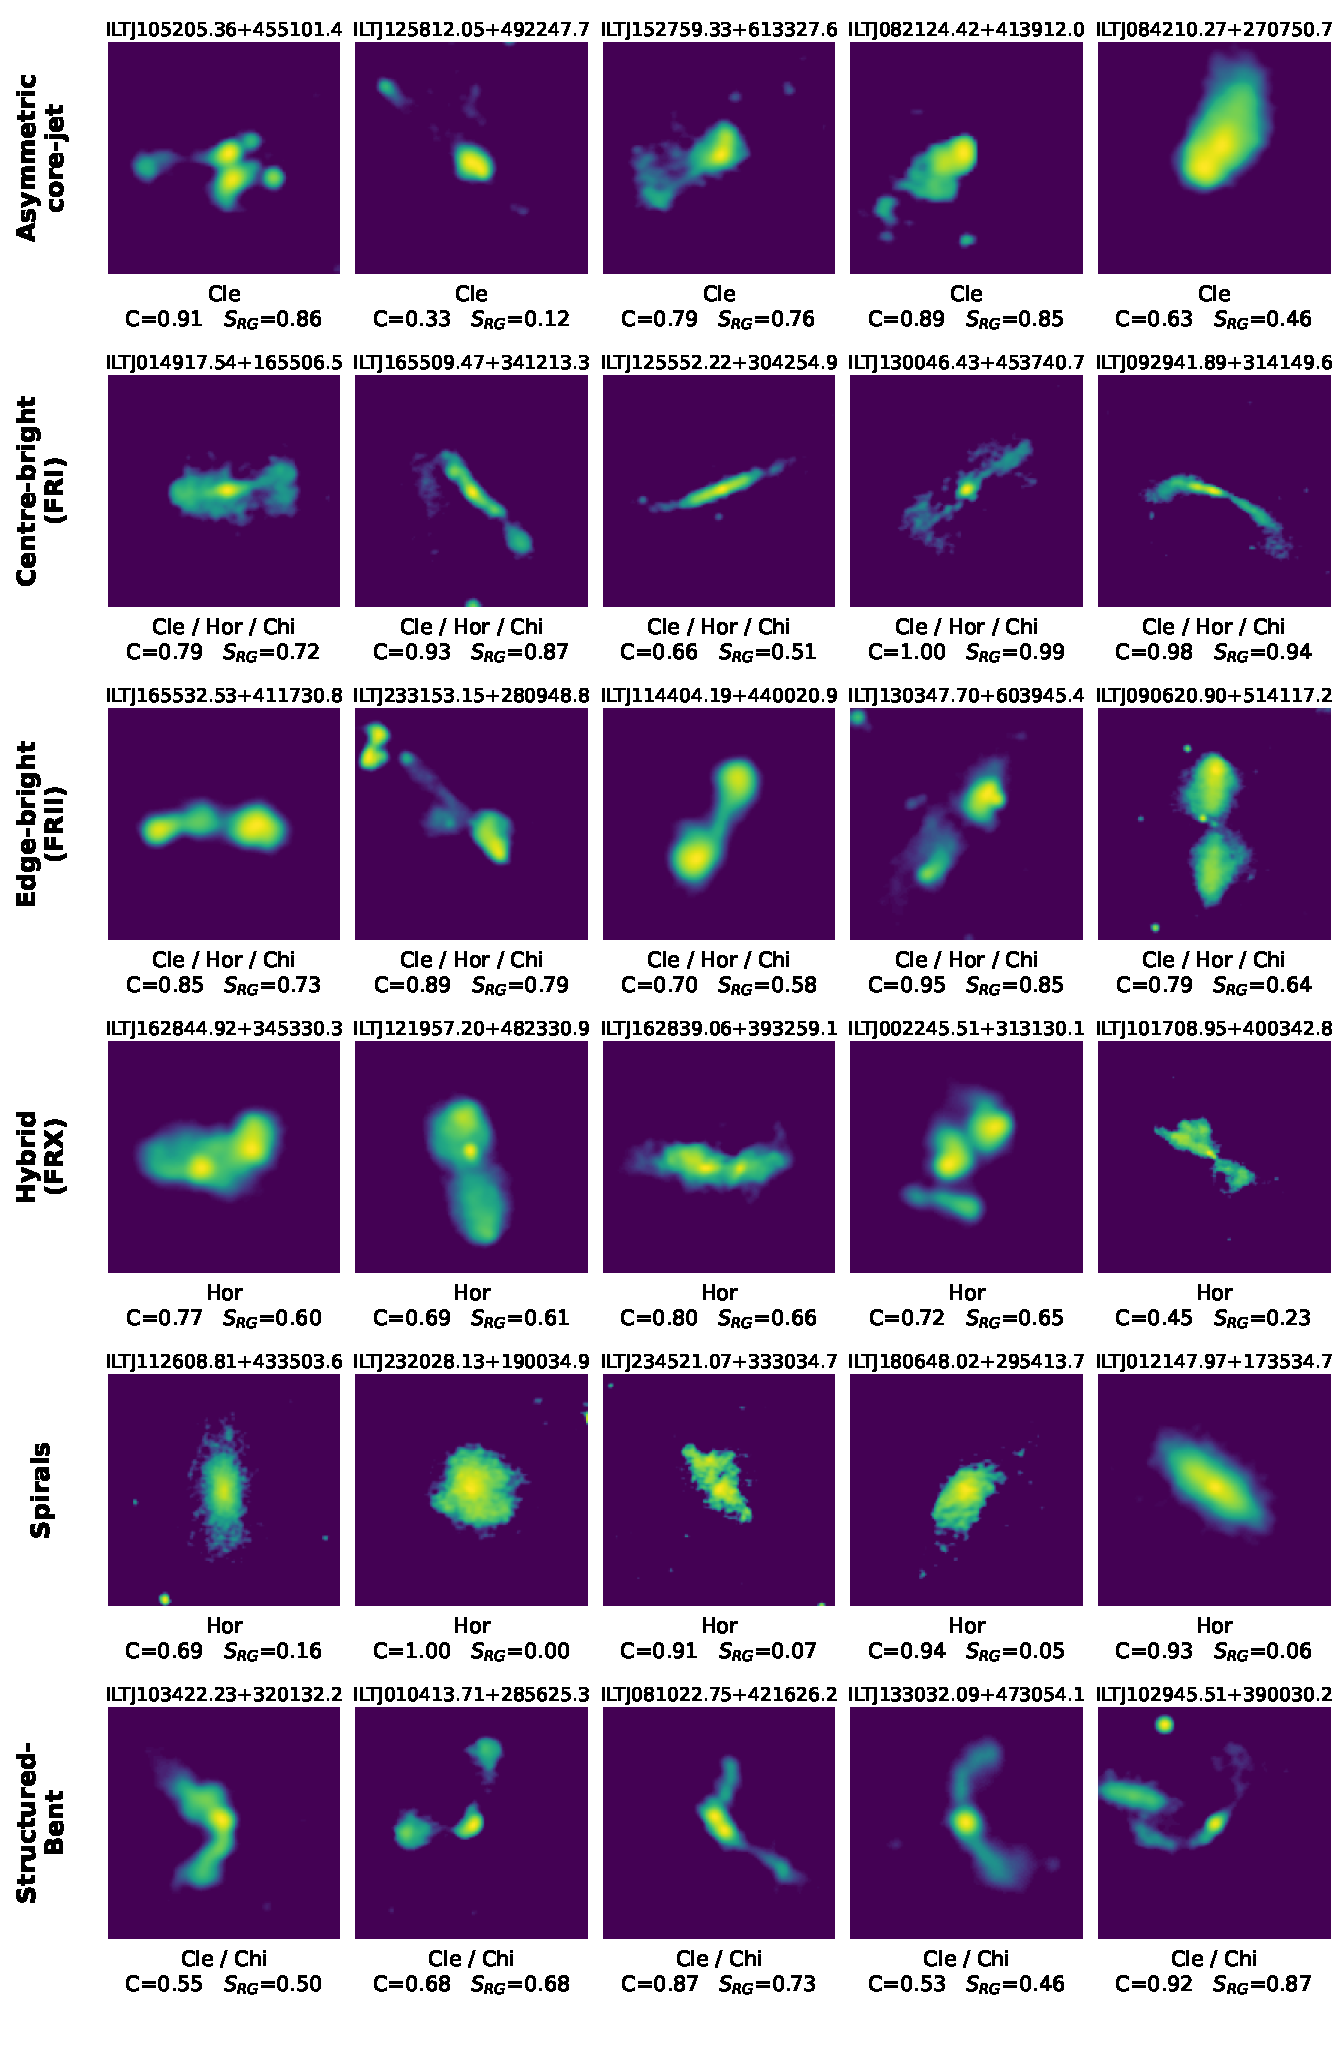
\includegraphics[width=\linewidth,height=0.90\textheight,keepaspectratio]{img/external_agreement_gallery.pdf}
\caption[Examples of agreement with external catalogues]{Agreement examples grouped by ensemble class. Cle, Hor, and Chi identify supporting catalogues. \(C\) denotes confidence and \(S_\mathrm{RG}\) the morphology score.}
\label{fig:agree_gallery}
\end{figure}

\subsection{Application to radio relics}
\label{sec:results_relics}

In order to test the model's response to the isolated diffuse emission, we apply the \(50\)-member ensemble to the ten selected, polygon-masked relic cutouts listed in Table~\ref{tab:relic_sample}. Detailed preprocessing is described in Sec.~\ref{sec:method_relics}.
Figure~\ref{fig:relic_grid} shows the actual inputs. Identification of relics in unmasked survey fields using an automated approach is a challenging task and lies beyond the scope of this work.

\begin{figure}[H]
\centering
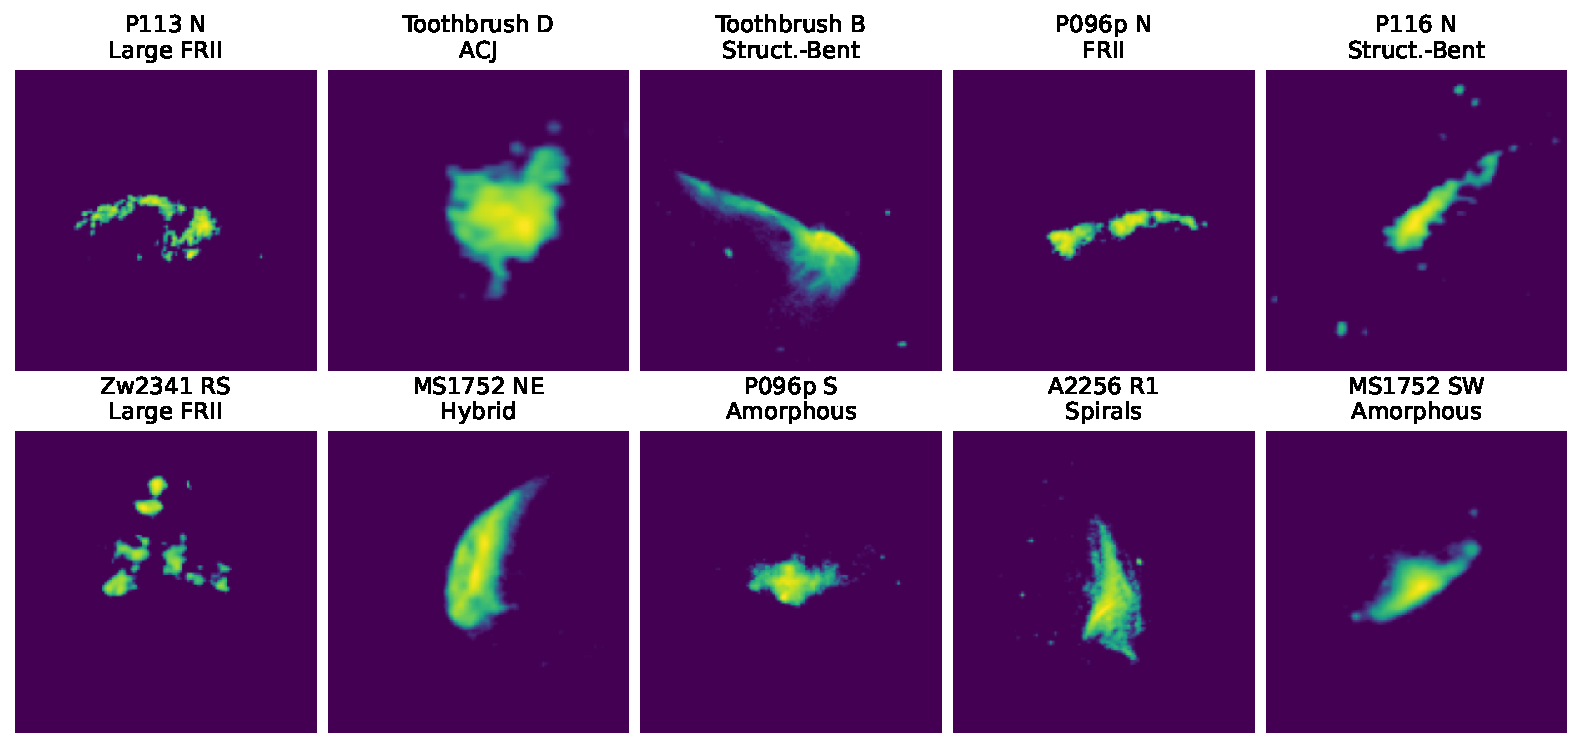
\includegraphics[width=\linewidth]{img/relic_image_grid.pdf}
\caption[Masked radio-relic inputs and predicted classes]{The ten masked relic inputs, shown in decreasing \(S_\mathrm{RG}\) order with their predicted morphology labels.}
\label{fig:relic_grid}
\end{figure}

\begin{table}[H]
\centering
\small
\setlength{\tabcolsep}{4pt}
\begin{tabular}{llrrrrrr}
\toprule
Relic & Predicted class & \(C\) & \(A\) & \(H\) & \(MI\) & \(P_\mathrm{RG}\) & \(S_\mathrm{RG}\) \\
\midrule
P113 N & Large FRII & 0.892 & 0.960 & 0.431 & 0.108 & 0.994 & 0.748 \\
Toothbrush D & ACJ & 0.739 & 1.000 & 0.863 & 0.058 & 0.941 & 0.588 \\
Toothbrush B & Structured-Bent & 0.637 & 0.980 & 0.974 & 0.035 & 0.991 & 0.568 \\
MS1752 SW & Amorphous & 0.489 & 0.780 & 1.436 & 0.091 & 0.267 & 0.080 \\
MS1752 NE & Hybrid & 0.590 & 0.780 & 0.800 & 0.074 & 0.613 & 0.309 \\
Zw2341 RS & Large FRII & 0.676 & 0.700 & 0.956 & 0.443 & 0.990 & 0.340 \\
P096p N & FRII & 0.689 & 0.840 & 0.942 & 0.195 & 0.989 & 0.464 \\
P096p S & Amorphous & 0.801 & 0.960 & 0.833 & 0.122 & 0.180 & 0.107 \\
P116 N & Structured-Bent & 0.523 & 0.740 & 1.207 & 0.049 & 0.980 & 0.353 \\
A2256 R1 & Spirals & 0.887 & 1.000 & 0.497 & 0.014 & 0.103 & 0.082 \\
\bottomrule
\end{tabular}
\caption[Ensemble predictions and scores for selected relics]{Ensemble outputs for the selected relics. \(C\) denotes confidence; \(H\) and \(MI\) are in nats\protect\footnotemark.}
\label{tab:relics}
\end{table}
\footnotetext{One nat is the amount of information from an event with a probability of \(1/e\).}

The relics span seven predicted classes (Table~\ref{tab:relics}). None is assigned to Unresolved. These labels describe resemblance to structures learned from the radio-galaxy sample.
Four relics fall in the transitional band and six in the low band; none reaches the high-score band (Figure~\ref{fig:relic_srg}). P113 N has the highest score, just below the high-band boundary.

\begin{figure}[H]
\centering
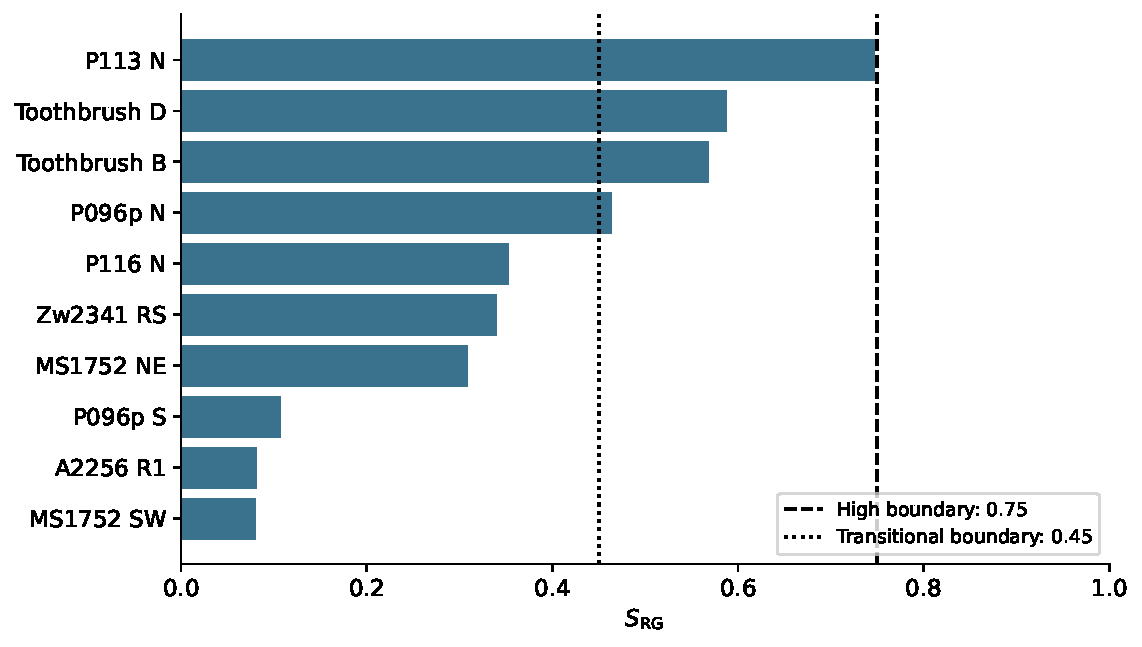
\includegraphics[width=0.9\linewidth]{img/relic_srg_bars.pdf}
\caption[Similarity scores for selected radio relics]{Similarity scores for the ten relics. Dashed and dotted lines mark the high and transitional boundaries, respectively.}
\label{fig:relic_srg}
\end{figure}

For Zw2341 RS, almost all probability lies in \(G\), yet uncertainty and disagreement among members reduce the final score. Conversely, A2256 R1 receives a confident and consistent Spirals assignment, which places it in \(N\) and gives a low score. These examples show how low scores can arise either from weaker reliability within the target groups or from concentrated support for a non-target class (Table~\ref{tab:relics}).

The retained arcs and elongated ridges can receive radio-galaxy-like assignments despite their different physical origin. The range of outputs demonstrates why neither high \(P_\mathrm{RG}\) nor low \(S_\mathrm{RG}\) alone identifies a relic. This visually selected sample does not establish relic-detection completeness or out-of-distribution performance, and the results remain conditional on the manual isolation and clipping of diffuse emission.



\cleartooddpage
\section{Discussion}
\label{sec:discussion}

In this chapter we discuss the model's morphological strengths and weaknesses, the use of its similarity score, and the main limits of the analysis.

\subsection{Morphological classification and external correspondence}
\label{sec:discussion_catalogue}
\label{sec:discussion_external}

By extending the approach of \citet{Nicolas2025}, we obtained a catalogue of \(32\,514\) sources with \(60''\leq\mathrm{LAS}\leq1000''\). Its eleven classes provide a common morphological description for selecting and inspecting this extended-source sample.

\citet{Nicolas2025} classified \(42\,230\) sources with LAS between \(30''\) and \(60''\) into twelve classes. We retain their host-centred image preparation and learning framework, while adopting a larger-angular-size sample and an eleven-class curation. The changed population and taxonomy prevent a direct comparison of classification performance.

We find stronger FRII than FRI correspondence against Clews and Horton, while performance is similar for the two classes against Chilufya (Tables~\ref{tab:ext_fri} and~\ref{tab:ext_frii}). These comparisons treat Edge-bright FRII and Large FRII as a single morphological family.

Frequent Bright-core assignments among reference FRI sources suggest that central brightness outweighs faint jets and lobes in the learned classification. Structured-Bent assignments suggest sensitivity to curvature, which some reference schemes include within FRI. Reference FRII sources assigned to Structured-Bent or Hybrid likewise suggest difficulty separating edge brightening from curvature and mixed structure (Figures~\ref{fig:ext_fn_fri} and~\ref{fig:ext_fn_frii}). 

The reference catalogues differ in source selection, classification method and available imaging \citep{Clews2025,Horton2025,Chilufya2025}. Similar FRI and FRII disagreements persist among the \(149\) sources whose mapped labels agree across all three catalogues, identifying cases that merit closer inspection (Sec.~\ref{sec:ext_consensus}). Most sources with fine-class disagreements receive a radio-galaxy-like label, although these labels also dominate the reference samples (Table~\ref{tab:ext_group_retention}).

Image preparation offers possible explanations for some disagreements: 
\begingroup
\setstretch{1.0}
\begin{itemize}[itemsep=2pt, parsep=0pt, topsep=3pt]
\item resampling cutouts to \(128\times128\) pixels can blur small features;
\item clipping can suppress faint emission, while linear intensity scaling leaves faint features weak relative to bright components;
\item neighbouring sources and host centring can also affect the structure presented to the model.
\end{itemize}
\endgroup
Thus, Bright-core and Core-Displaced assignments require inspection of the original radio field and host information for physical interpretation.

Unlike \citet{Nicolas2025}, we omitted active-pixel selection because it would substantially reduce the sample.
It could also exclude diffuse or extended sources, including some Large FRII sources, if too few pixels exceed the intensity threshold.

Visual cluster consolidation and SI-SSIM filtering help define the class boundaries (Sec.~\ref{sec:method_labels}). Their outcome depends on how carefully clusters are grouped into morphologically coherent classes and which examples are retained.

\subsection{Similarity scoring and diffuse-emission applications}
\label{sec:discussion_score}
\label{sec:discussion_relics}

The similarity score introduced here adds a filtering layer to the morphology catalogue by combining support for radio-galaxy-like (\(G\)) classes with ensemble reliability.
Its proposed use is to prioritise sources for inspection within the fitted model and adopted preprocessing.

The model already assigns \(92.5\,\%\) of the full sample to \(G\), so frequent \(G\) assignments among external disagreements are mainly a descriptive result.

In the mapped-reference sample, sources assigned to the non-target group \(N\) favour low \(P_\mathrm{RG}\) and remain below \(S_\mathrm{RG}=0.25\), including cases with high reliability (Figure~\ref{fig:ext_srg_distributions}). Within \(G\), reliability separates concentrated, consistent predictions from weaker support. Examining \(P_\mathrm{RG}\) and \(R\) separately shows which factor reduces the score. 

We should note that the score bands depend on the fitted model and the adopted \(G/N\) definitions. Independent review is needed to establish their selection quality and any improvement over \(P_\mathrm{RG}\) alone.

The ten selected relics receive seven morphology labels, illustrating how diffuse arcs and ridges can resemble structures learned from radio galaxies (Table~\ref{tab:relics}). All fall in the transitional or low-score bands, despite several having large \(P_\mathrm{RG}\). These results show that morphological resemblance can extend across physically different source populations.

Manual masking is important for isolating relic emission, while clipping and rescaling determine which features remain visible. The conclusions therefore apply to these deliberately prepared examples. Automated identification of radio relics or other diffuse emission in unmasked survey fields lies beyond this work's scope.

The polygon also changes the pixels used to estimate the clipping threshold, coupling source isolation to intensity preprocessing. P113 N lies just below the high-score boundary; its band assignment should therefore be tested against reasonable changes in masking and clipping.

\subsection{Limitations and implications for future work}
\label{sec:discussion_validation}

One limitation of the pipeline is its dependence on the source associations, host coordinates and angular sizes supplied by the value-added catalogue.
Errors in these quantities can affect sample membership, cutout centring and the extent of emission included in the model input.
Applying the pipeline to another survey requires equivalent source associations, host positions and angular-size estimates.

Another bottleneck of the framework is manual curation, which is time-consuming and depends on the analyst's judgement.
Reproducibility requires preserving the original cluster memberships, cluster-to-class mapping and filtering choices; in Appendix~\ref{app:hdbscan_cluster_overview} we record the grouping used in this work. Independent repeat curation would test the stability of the class boundaries.

The validation and test sets used for fine-tuning contain only \(22\) and \(33\) sources, making performance estimates for individual classes uncertain.
Their selection from the curated sample also favours the morphologies retained by the filtering procedure.
External comparisons use independently assigned reference labels, although some compared sources were used for classifier training (Sec.~\ref{sec:results_external}).

The main evaluation priority is an independently reviewed sample covering all classes, score bands and angular sizes. Testing on additional sky fields would assess transfer beyond the population used for pre-training.

Agreement also varies with angular size: against Horton, FRI recovery is weakest among the smallest sources (Table~\ref{tab:las_sensitivity}). Under the adopted resampling, a \(6''\) beam spans approximately \(512/\mathrm{LAS}\) pixels, with LAS expressed in arcseconds, decreasing from \(8.53\) to \(0.512\) pixels across the sample's size range and limiting the preservation of small-scale structure in the largest sources. Since morphology and resolution vary together, controlled tests of intensity scaling, source isolation and angular-size dependence would help distinguish their contributions to the observed disagreements, as outlined in Chapter~\ref{sec:conclusion}.


\cleartooddpage
\section{Conclusion and Outlook}
\label{sec:conclusion}

\subsection{Main conclusions}

\begingroup
\emergencystretch=2em
We produced an eleven-class catalogue of \(32\,514\) extended LoTSS-DR2 sources using the adapted framework of \citet{Nicolas2025}. Self-supervised pre-training, cluster curation and a \(50\)-member ensemble provide morphology assignments and uncertainty summaries.
\par
\endgroup

FRII correspondence is stronger than FRI correspondence against Clews and Horton, while the two are similar against Chilufya. FRI recovery remains weak, identifying an important limitation of the learned classification (Sec.~\ref{sec:results_external}).

The inspection score \(S_\mathrm{RG}\) combines radio-galaxy-like probability mass with ensemble reliability, distinguishing broad morphological support from concentrated and consistent predictions. Classes, score components and cutouts should be inspected together.

Among ten selected, masked relics, none reaches the high-score boundary.
Their varied morphology assignments illustrate the model's response to deliberately isolated diffuse emission.

\subsection{Future work}

Independent review across classes and score bands should assess the quality of score-based selections and probability calibration against observed correctness \citep{Guo2017}. It should include sources outside the curated sample.

PyBDSF catalogue positions and fitted sizes offer a possible route to applying the pipeline without host identifications. \citet[Sec.~2]{Nicolas2026} centre DR3 cutouts on radio mean positions and use a side length of \(2.5\times\mathrm{Maj}\), where \(\mathrm{Maj}\) is the fitted Gaussian major axis. 
Comparing these radio-centred inputs with our host-centred cutouts would test the sensitivity to source association, centring and size estimates.

Controlled retraining should compare intensity scaling and automatic source isolation on a fixed, independently reviewed sample. LAS-stratified performance would inform size-specific modelling, accounting for the smaller samples at large angular sizes.

Synthetic core-and-lobe images could also test sensitivity to central brightness, bending and faint extended emission, following the pre-training evaluation of \citet{Nicolas2025}. Any resulting training changes should be assessed on real sources, particularly reference FRI examples.

A broader relic sample with controlled masking and clipping variants would test how input preparation affects the predictions. Including unmasked fields, radio haloes and revived fossil plasma would extend the assessment to more varied diffuse-emission environments \citep{vanWeeren2019}.

\subsection{Data and software availability}
\label{sec:availability}

The final source catalogue, trained classification model and author-developed analysis tools, including the polygon-masking interface, are available upon request; the inherited learning framework is credited separately in Chapter~\ref{sec:intro}. Requests can be directed to \href{mailto:harutyunianedgar@gmail.com}{\nolinkurl{harutyunianedgar@gmail.com}}.


\cleartooddpage
\appendix
\section{GreyResNet18 encoder and projection head}
\label{app:greyresnet18_architecture}

\begin{figure}[H]
  \centering
  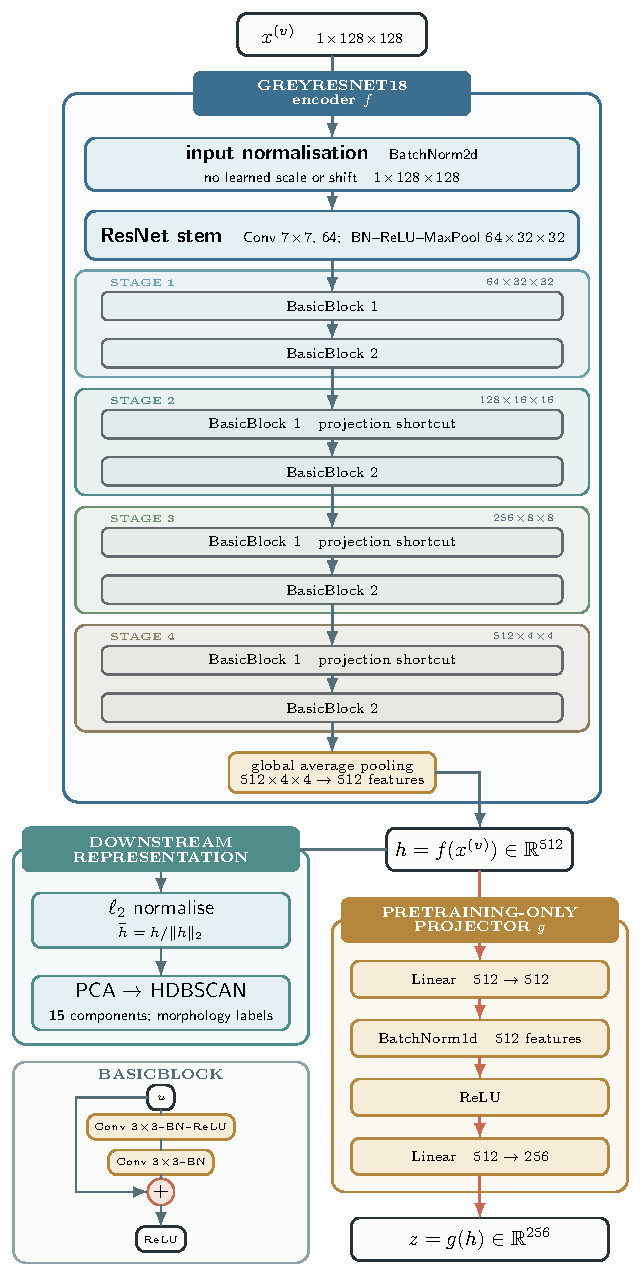
\includegraphics[
    width=\linewidth,
    height=0.72\textheight,
    keepaspectratio
  ]{img/greyresnet18_projector_architecture.pdf}
  \caption[GreyResNet18 encoder and projection head]{GreyResNet18 encoder and projection head used for contrastive
    pre-training, shown for one generic augmented view \(x^{(v)}\); both SimCLR
    views pass through the same encoder and projector parameters. In the
    ResNet stem, the \(7\times7\) convolution and max-pooling operation both
    use stride \(2\). The first BasicBlock of stages 2--4 halves the spatial
    resolution: its first \(3\times3\) convolution and its \(1\times1\)
    projection shortcut use stride \(2\), whereas the remaining BasicBlocks
    use stride \(1\) and identity shortcuts. Global average pooling is
    implemented by adaptive average pooling followed by flattening, producing
    the \(512\)-dimensional representation \(h\). The projection head \(g\) is
    used only during pre-training and maps \(h\) to the \(256\)-dimensional
    projection \(z\); it is discarded for downstream analysis.}
  \label{fig:greyresnet18_architecture}
\end{figure}

\clearpage
\section{Raw PCA--HDBSCAN cluster overview}
\label{app:hdbscan_cluster_overview}

Figures~\ref{fig:hdbscan_cluster_overview_first} and~\ref{fig:hdbscan_cluster_overview_second} show the raw groups used during manual inspection, with actual HDBSCAN labels \(-1,0,\ldots,58\). Table~\ref{tab:cluster_class_mapping} records their consolidation into the eleven morphology classes.

\begin{figure}[H]
  \centering
  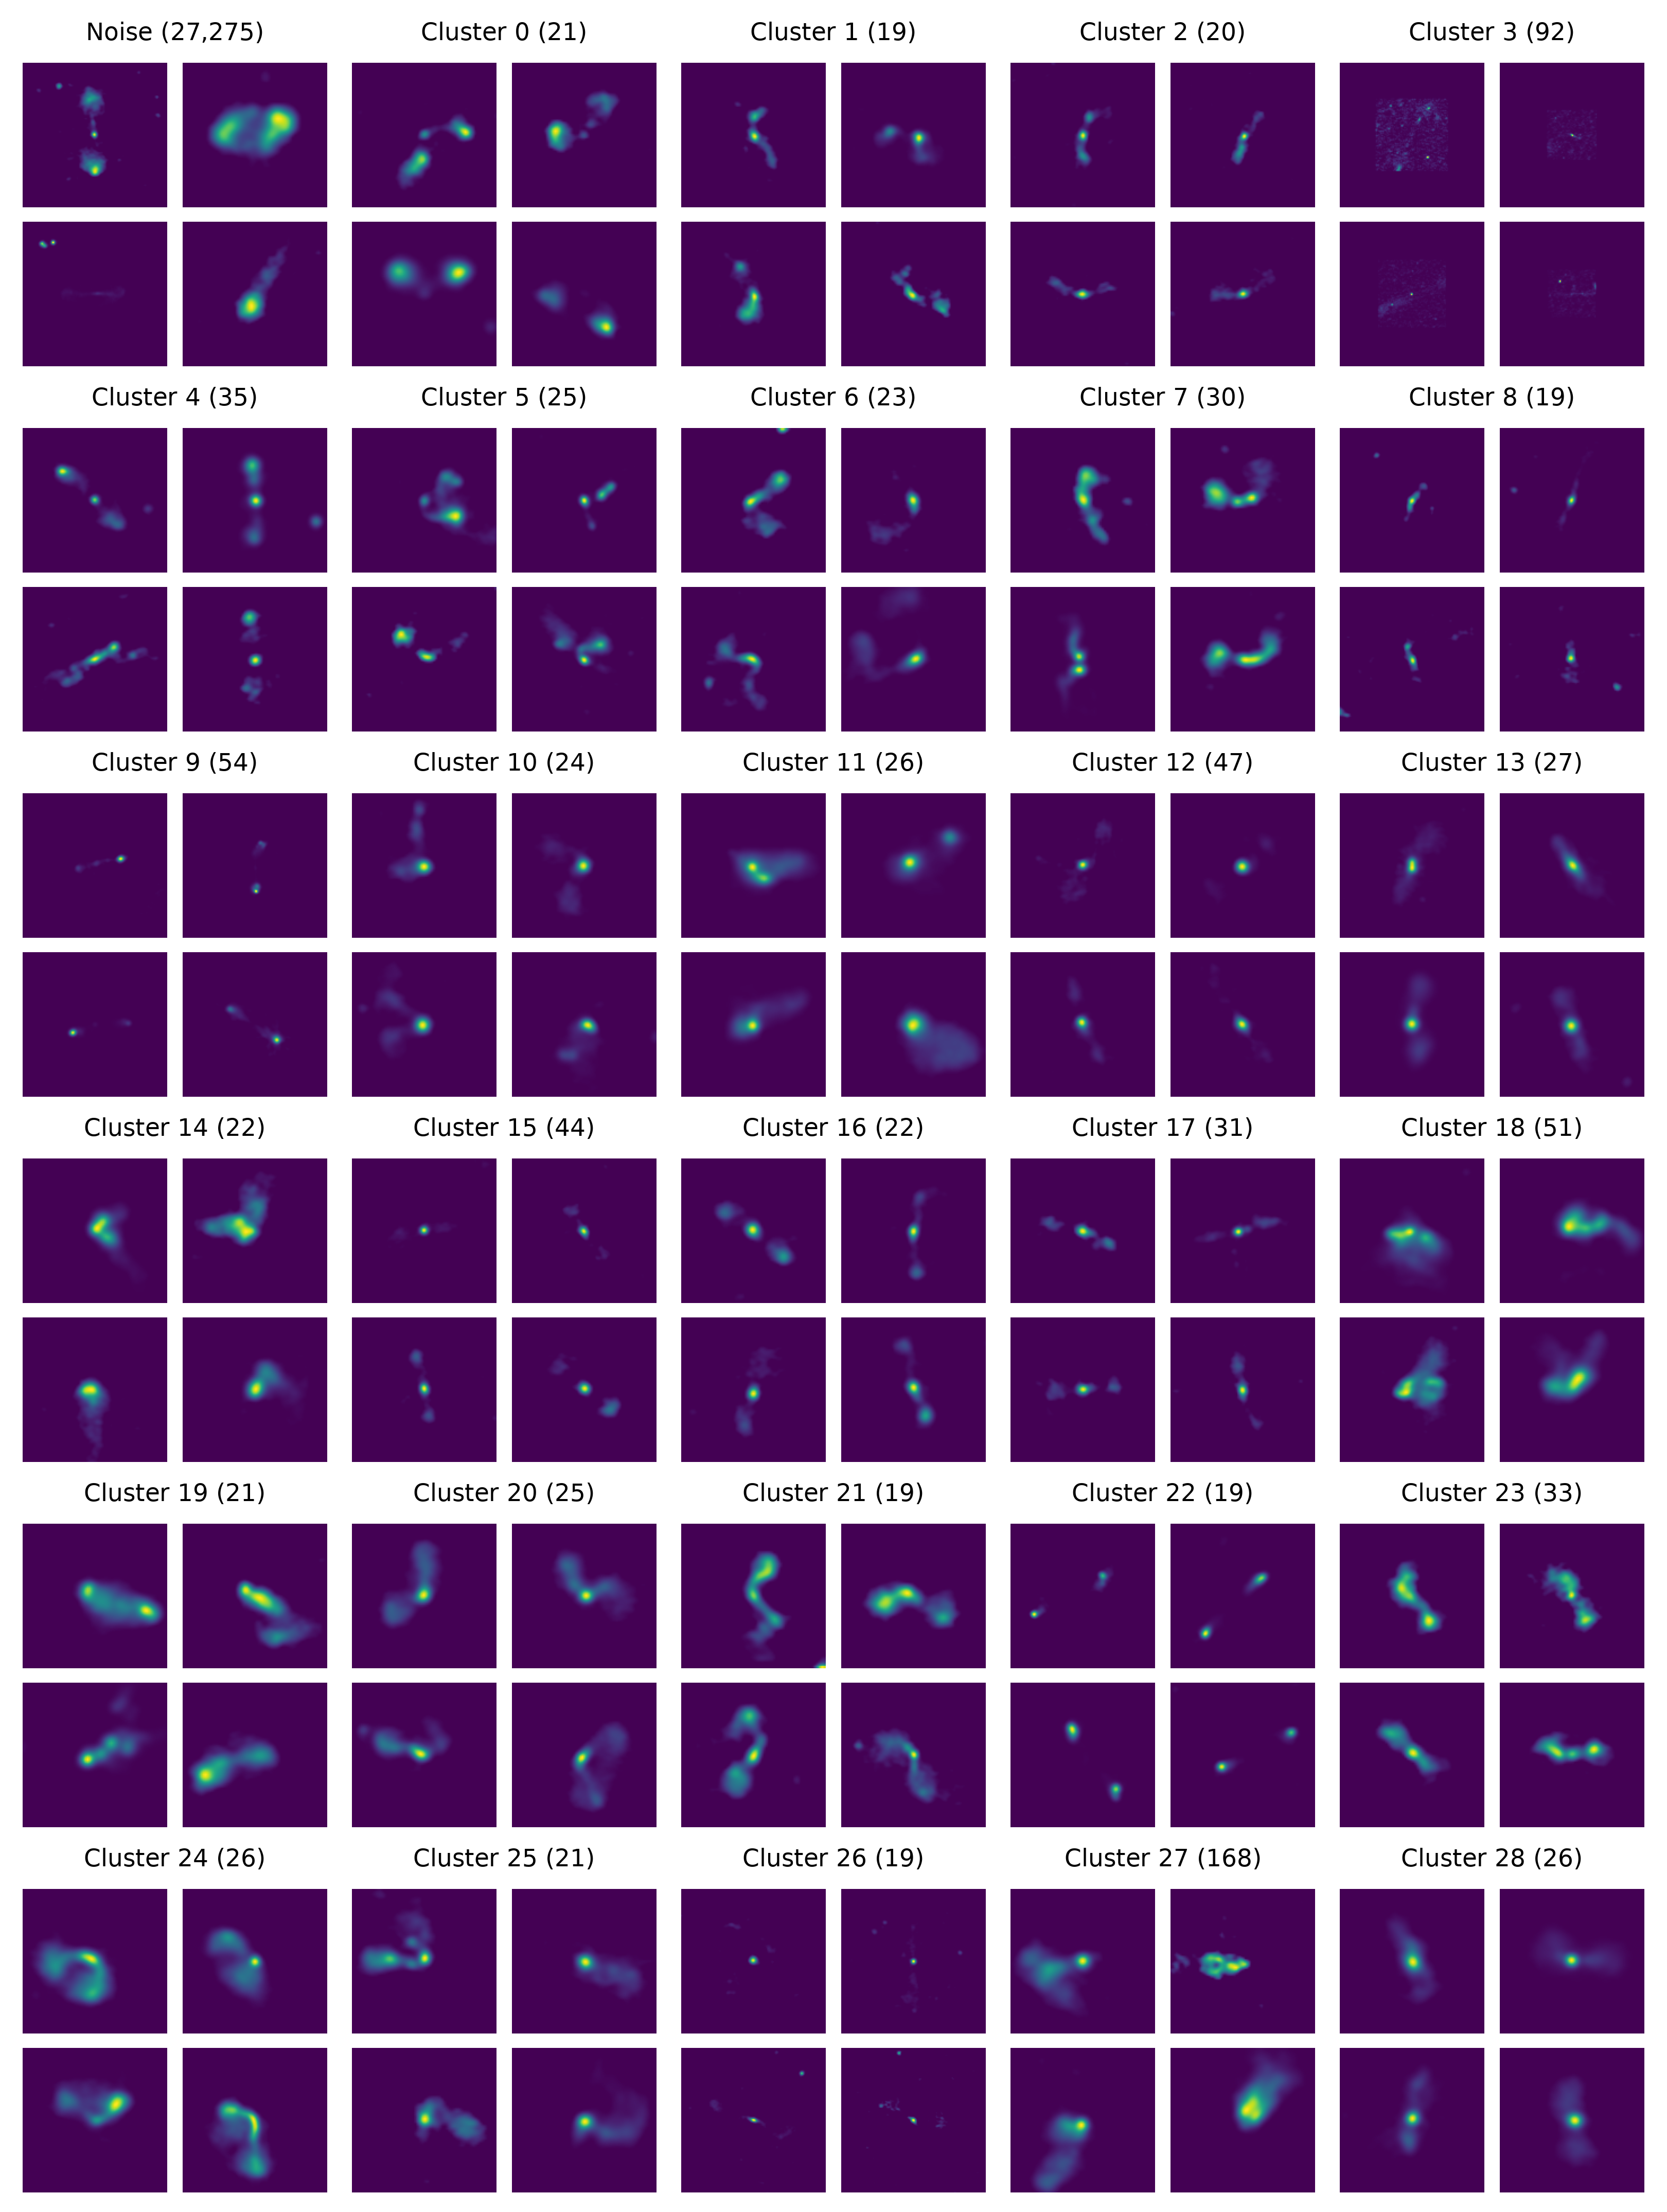
\includegraphics[width=\linewidth,height=0.73\textheight,keepaspectratio]{img/hdbscan_cluster_portrait_noise_28.png}
  \caption[HDBSCAN overview: noise and clusters 0--28]{Noise group \(-1\) and clusters 0--28, read left to right and top to bottom. Each group shows four examples; parentheses give its total membership.}
  \label{fig:hdbscan_cluster_overview_first}
\end{figure}
\clearpage
\begin{figure}[p]
  \centering
  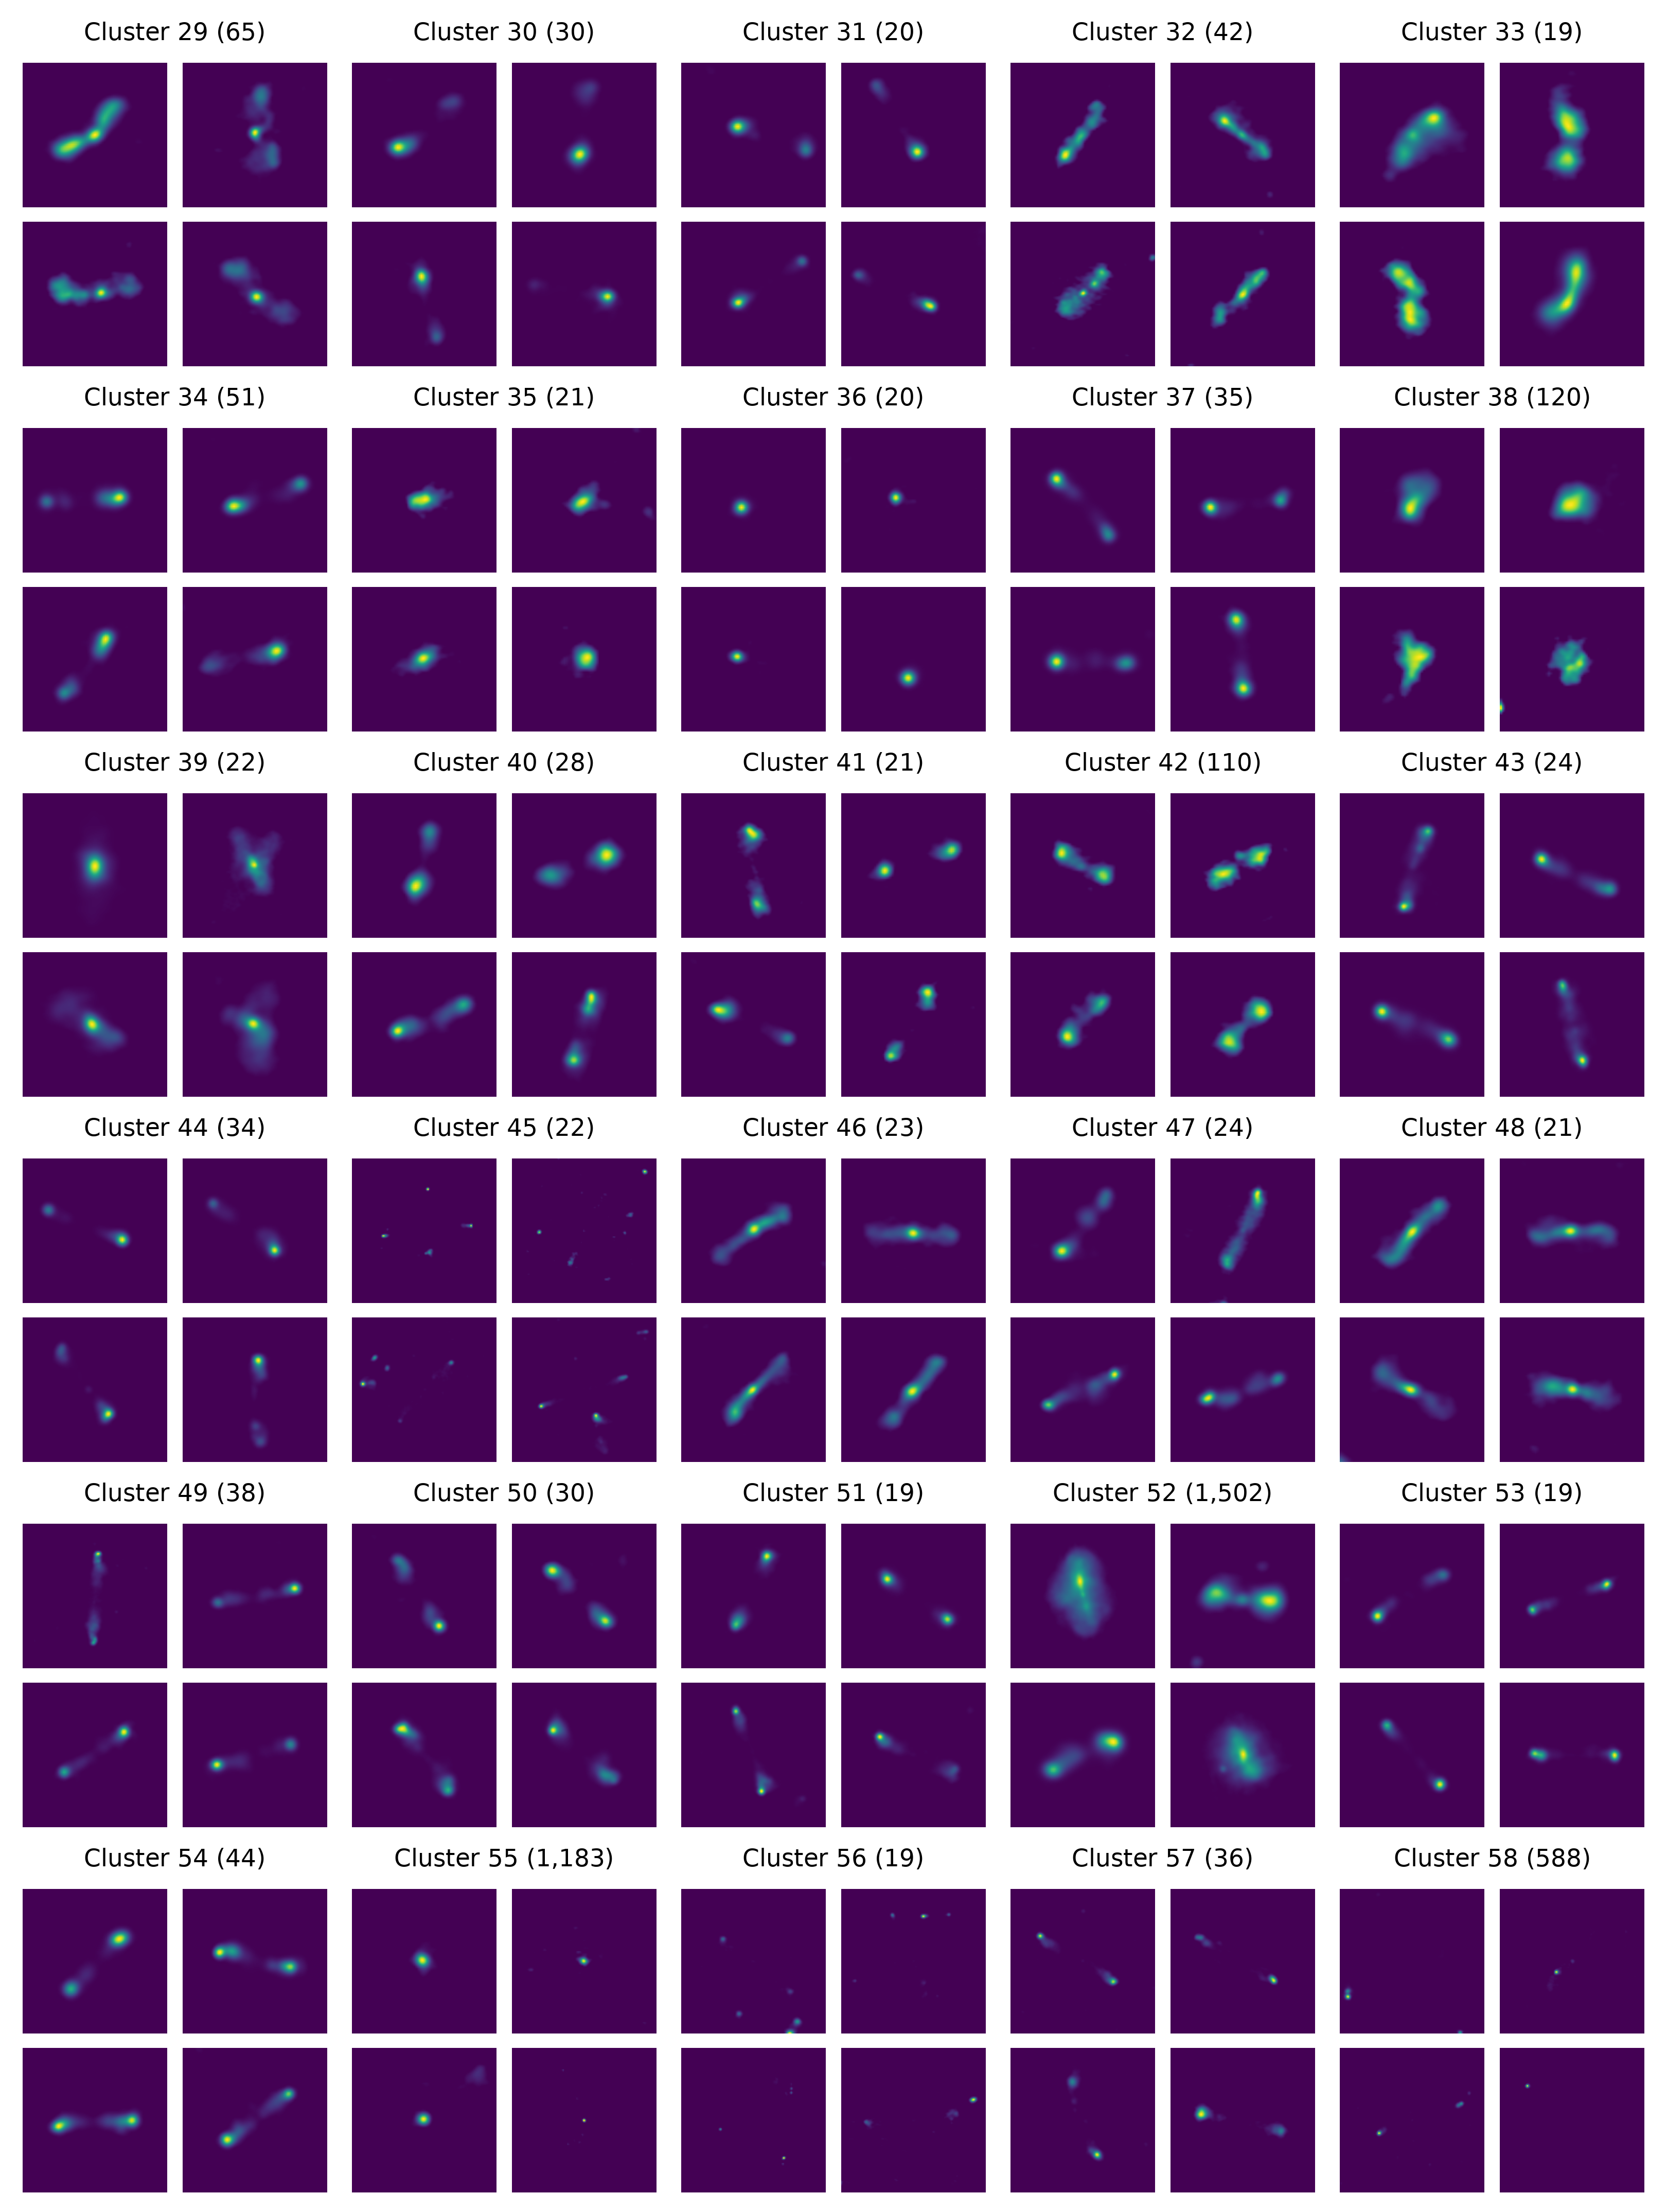
\includegraphics[width=\linewidth,height=0.83\textheight,keepaspectratio]{img/hdbscan_cluster_portrait_29_58.png}
  \caption[HDBSCAN overview: clusters 29--58]{Clusters 29--58, in the same format as Figure~\ref{fig:hdbscan_cluster_overview_first}.}
  \label{fig:hdbscan_cluster_overview_second}
\end{figure}
\clearpage

\begin{table}[H]
\centering
\small
\setlength{\tabcolsep}{4pt}
\begin{tabular}{@{}lp{0.48\linewidth}r@{}}
\toprule
Morphology class & Raw HDBSCAN labels & Sources \\
\midrule
Amorphous & 35 & 21 \\
ACJ & 11, 14 & 48 \\
Bright-core & 55 & 1\,183 \\
Centre-bright FRI & 2, 4, 8, 12, 13, 15, 16, 17, 26, 28, 46, 48 & 334 \\
Core-Displaced & 36 & 20 \\
Edge-bright FRII & 22, 30, 31, 34, 37, 40, 41, 42, 43, 44, 47, 49, 50, 51, 53, 54 & 546 \\
Hybrid & 23, 32 & 75 \\
Large FRII & 9, 57 & 90 \\
Spirals & 38 & 120 \\
Structured-Bent & 0, 1, 5, 6, 7, 10, 20, 21, 24, 25, 29 & 298 \\
Unresolved & 3, 45, 56, 58 & 721 \\
\midrule
Returned to unassigned & 18, 19, 27, 33, 39, 52 & 1\,783 \\
Original noise & \(-1\) & 27\,275 \\
\bottomrule
\end{tabular}
\caption[Raw-cluster consolidation into morphology classes]{Raw-cluster consolidation before SI-SSIM filtering. Every raw label occurs once; source counts sum to \(32\,514\).}
\label{tab:cluster_class_mapping}
\end{table}


\clearpage
\section{Examples of external-label disagreement}
\label{app:external_disagreements}

Figures~\ref{fig:disagree_gallery}--\ref{fig:disagree_gallery_3} show five examples per internal class with at least one mapped-label disagreement. Selection favours reference coverage and label diversity. Row labels give ensemble predictions; Cle, Hor, and Chi denote Clews, Horton, and Chilufya, with a dash for missing mapped labels. \(C\) denotes confidence. The two internal FRII classes remain separate in this inspection sample.

\begin{figure}[H]
\centering
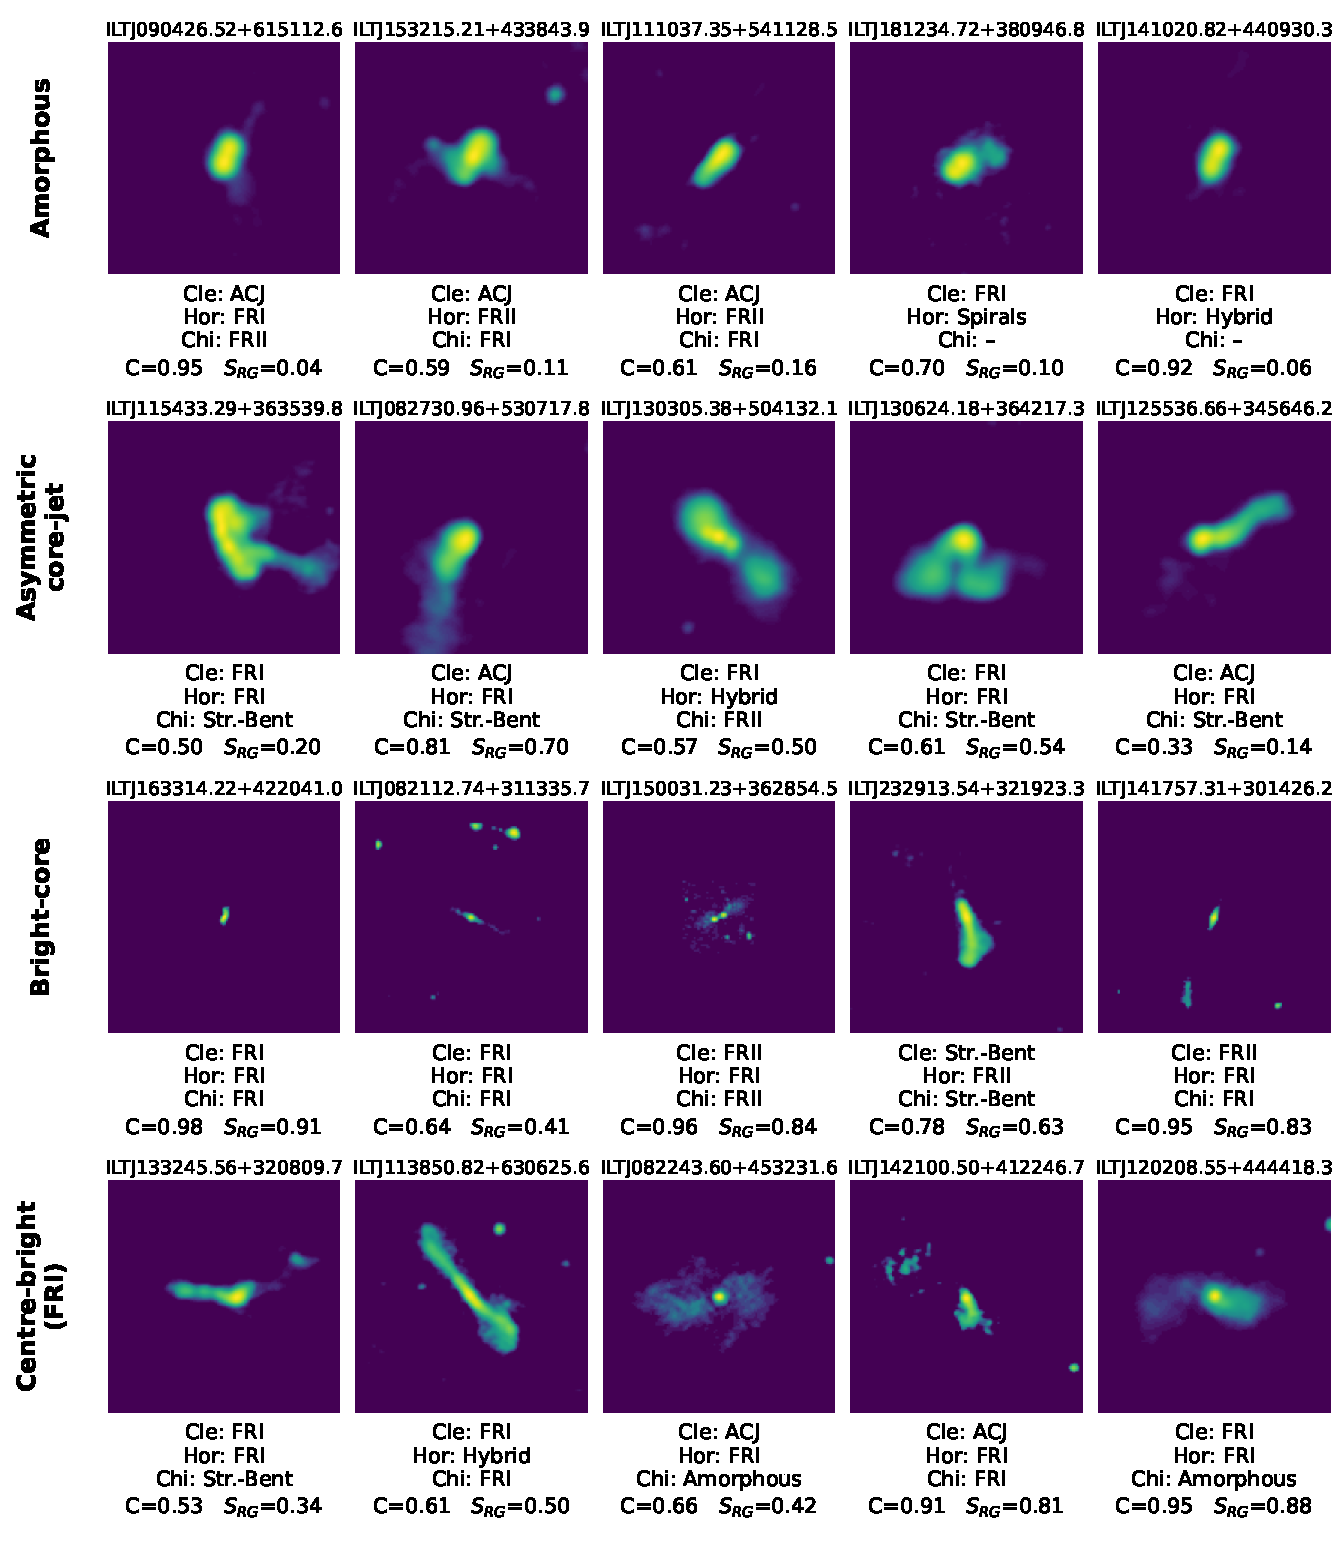
\includegraphics[width=\linewidth,height=0.73\textheight,keepaspectratio]{img/disagreement_gallery_1.pdf}
\caption[External disagreements: Amorphous, ACJ, Bright-core and FRI]{Five disagreement examples per class for Amorphous, ACJ, Bright-core, and FRI.}
\label{fig:disagree_gallery}
\end{figure}

\begin{figure}[p]
\centering
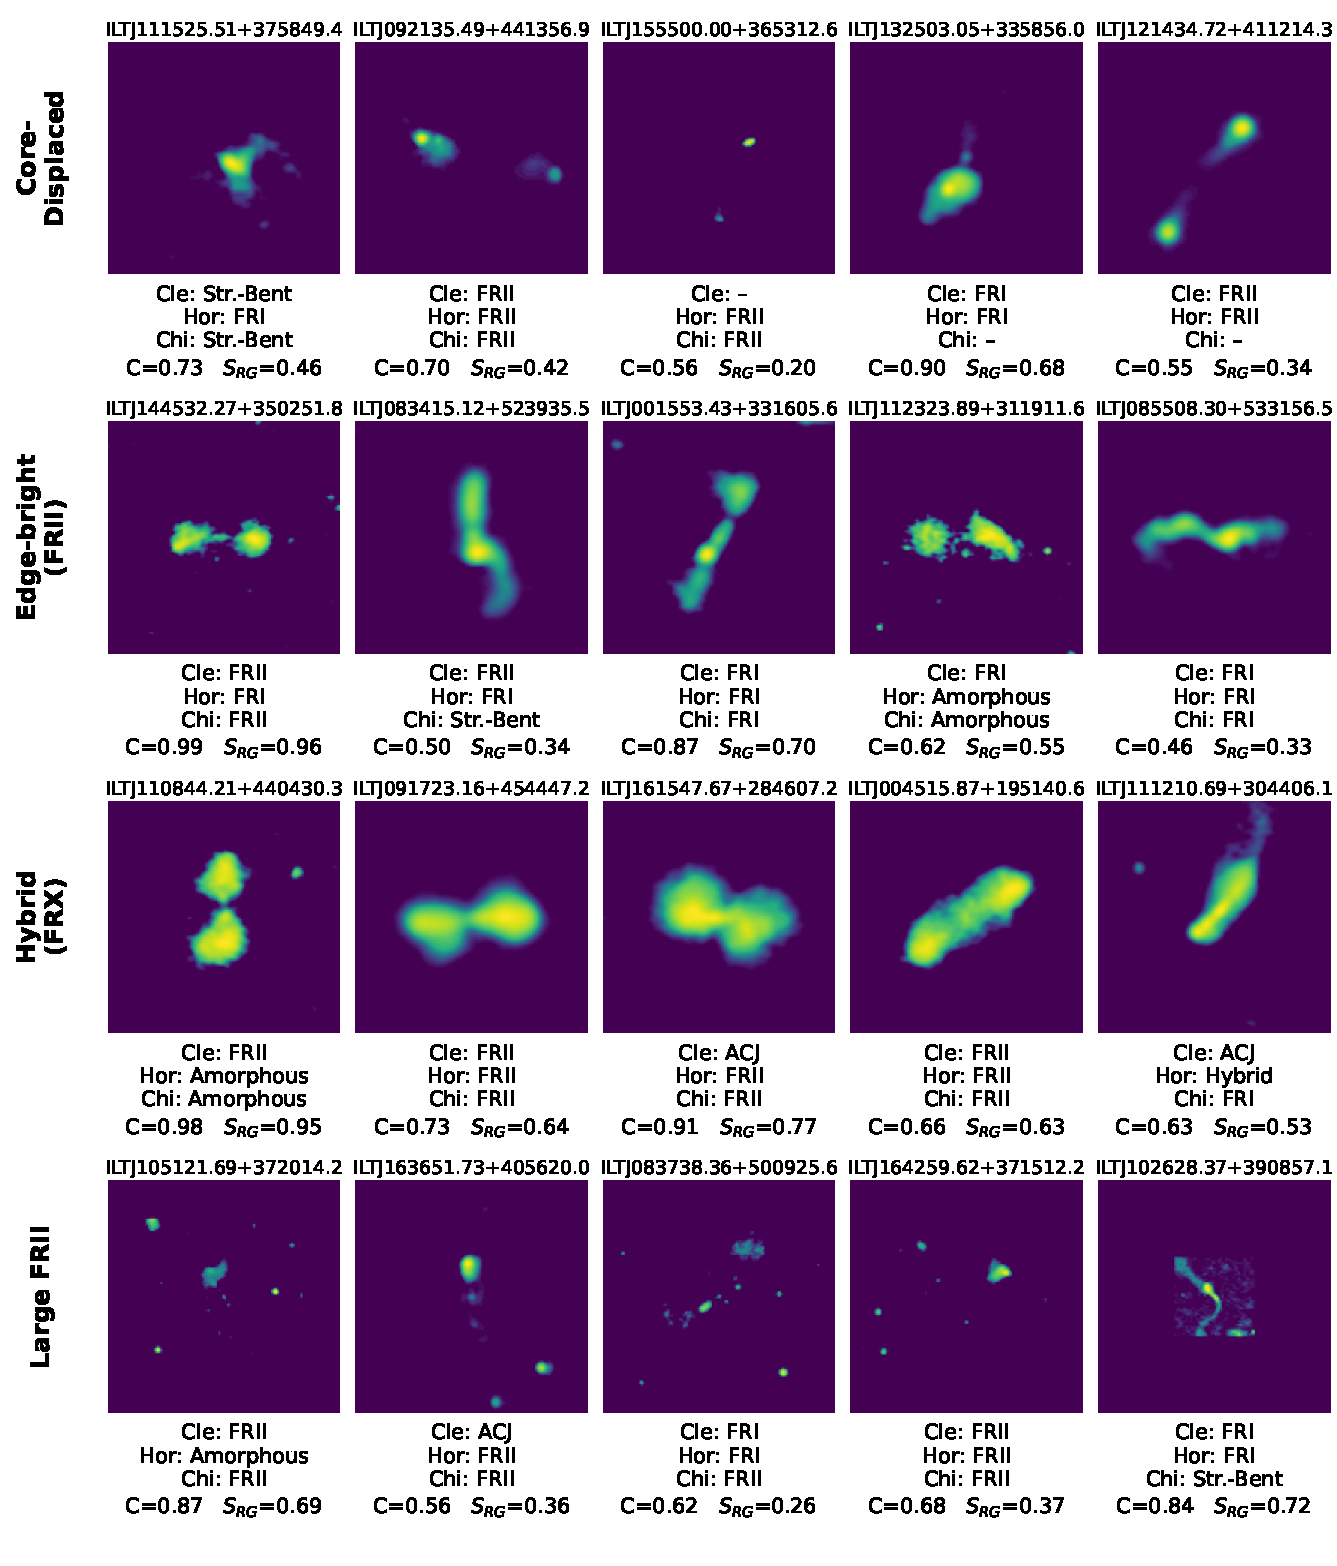
\includegraphics[width=\linewidth,height=0.87\textheight,keepaspectratio]{img/disagreement_gallery_2.pdf}
\caption[External disagreements: Core-Displaced, FRII, Hybrid and Large FRII]{Disagreement examples for Core-Displaced, FRII, Hybrid, and Large FRII. Annotations follow Figure~\ref{fig:disagree_gallery}.}
\label{fig:disagree_gallery_2}
\end{figure}

\begin{figure}[p]
\centering
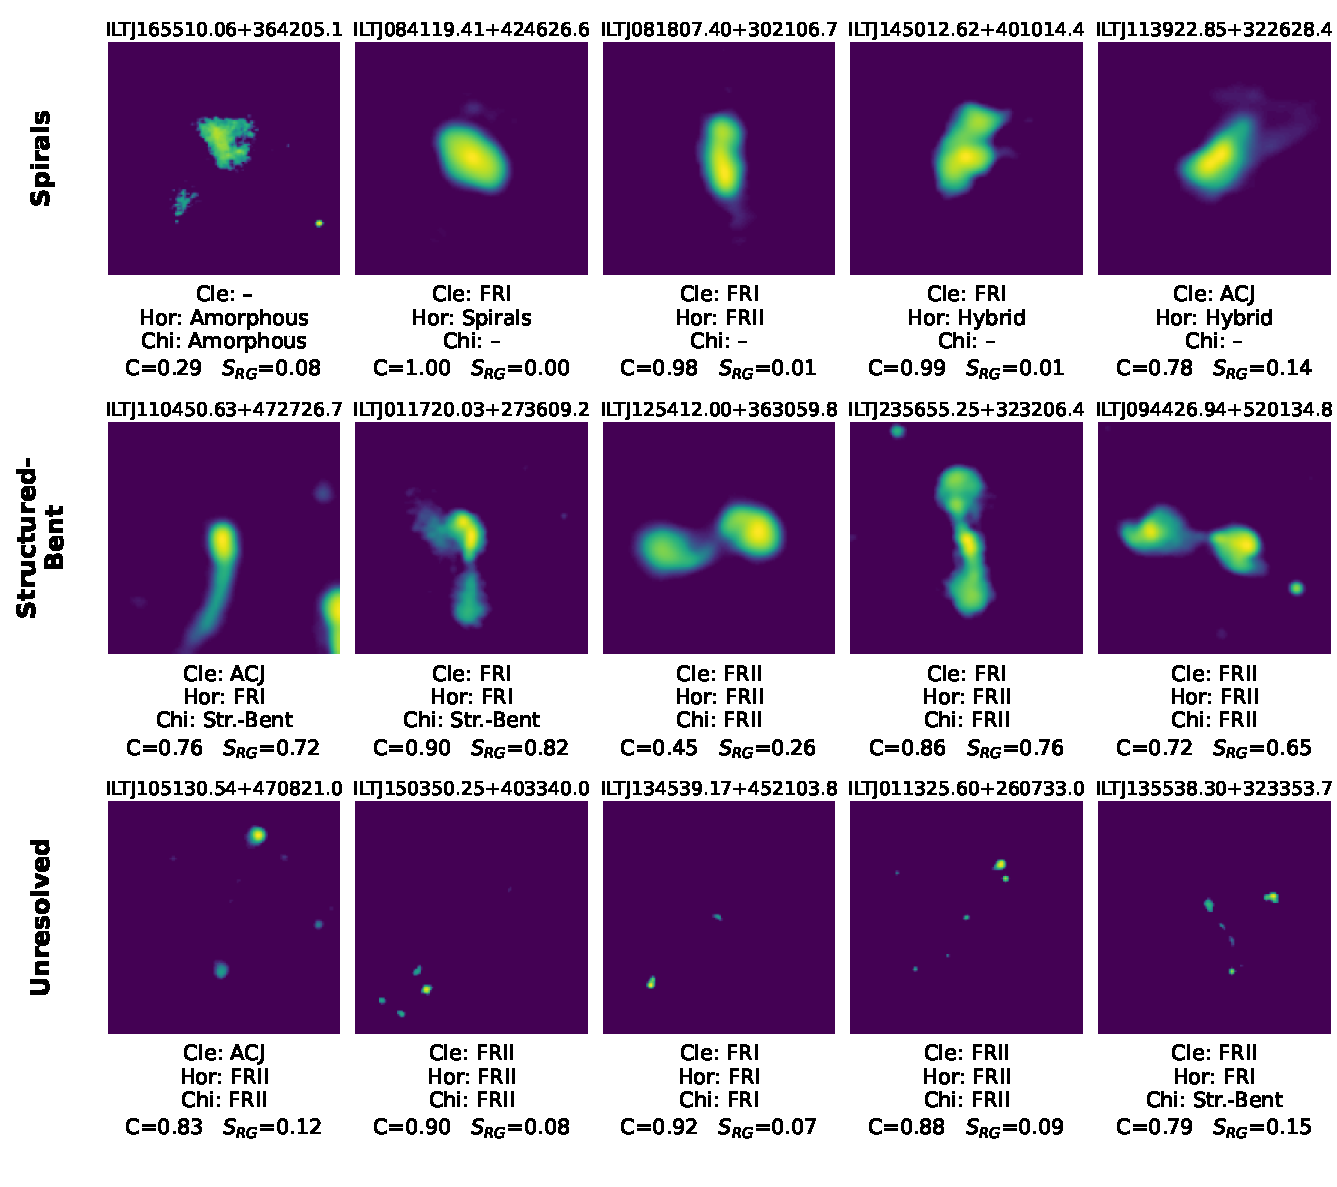
\includegraphics[width=\linewidth,height=0.87\textheight,keepaspectratio]{img/disagreement_gallery_3.pdf}
\caption[External disagreements: Spirals, Structured-Bent and Unresolved]{Disagreement examples for Spirals, Structured-Bent, and Unresolved. Annotations follow Figure~\ref{fig:disagree_gallery}.}
\label{fig:disagree_gallery_3}
\end{figure}


\clearpage
\begingroup
\setstretch{1.1}
\section{Supplementary evaluation}
\label{app:evaluation}

The test-set counts in Table~\ref{tab:heldout_counts} use the same ensemble as the main catalogue. Each reference class contains three test sources; the source-level predictions and full confusion matrix are retained with the accompanying analysis outputs.

\begin{table}[H]
\centering
\small
\setstretch{1}
\begin{tabular}{@{}lrrl@{}}
\toprule
Reference class & Test sources & Correct & Other assignments \\
\midrule
Amorphous & 3 & 3 & -- \\
ACJ & 3 & 1 & Spirals (1), Structured-Bent (1) \\
Bright-core & 3 & 3 & -- \\
FRI & 3 & 2 & Hybrid (1) \\
Core-Displaced & 3 & 3 & -- \\
FRII & 3 & 3 & -- \\
Hybrid & 3 & 3 & -- \\
Large FRII & 3 & 3 & -- \\
Spirals & 3 & 3 & -- \\
Structured-Bent & 3 & 1 & ACJ (2) \\
Unresolved & 3 & 3 & -- \\
\bottomrule
\end{tabular}

\caption[Test-set classification counts]{Predictions for the \(33\) test sources.}
\label{tab:heldout_counts}
\end{table}

The \(F_1\) uncertainties in the main comparison tables and Table~\ref{tab:las_sensitivity} use source-level bootstrap resampling: for each catalogue separately, we repeatedly draw samples of the original size, allowing a source to be selected more than once. Each selected source retains its reference label and saved model prediction, and we recalculate \(F_1\) for each sample without retraining the model. The central \(95\,\%\) of the resulting \(F_1\) values defines the reported uncertainty interval.

Signed uncertainties give the distances from each estimate to its lower and upper \(95\,\%\) interval bounds. They describe sampling variation within the selected samples, excluding uncertainty in reference labels, source selection and training. FRII includes both internal FRII classes, as in the main comparisons.

\begin{table}[H]
\centering
\small
\setstretch{1}
\setlength{\tabcolsep}{5pt}
\renewcommand{\arraystretch}{1.6}
\begin{tabular}{@{}llrrr@{}}
\toprule
Catalogue & LAS (arcsec) & Sources & FRI \(F_1\) & FRII \(F_1\) \\
\midrule
Clews & 60--120 & 6002 & \(0.310_{-0.024}^{+0.024}\) & \(0.739_{-0.014}^{+0.013}\) \\
Horton & 60--120 & 4635 & \(0.120_{-0.025}^{+0.026}\) & \(0.772_{-0.012}^{+0.011}\) \\
Chilufya & 60--120 & 1420 & \(0.388_{-0.059}^{+0.057}\) & \(0.378_{-0.046}^{+0.044}\) \\
Clews & 120--240 & 1539 & \(0.562_{-0.036}^{+0.035}\) & \(0.739_{-0.032}^{+0.029}\) \\
Horton & 120--240 & 2868 & \(0.383_{-0.032}^{+0.033}\) & \(0.719_{-0.019}^{+0.018}\) \\
Chilufya & 120--240 & 906 & \(0.490_{-0.051}^{+0.050}\) & \(0.521_{-0.055}^{+0.051}\) \\
Clews & 240--1000 & 216 & \(0.419_{-0.105}^{+0.093}\) & \(0.583_{-0.099}^{+0.092}\) \\
Horton & 240--1000 & 849 & \(0.363_{-0.055}^{+0.054}\) & \(0.605_{-0.045}^{+0.042}\) \\
Chilufya & 240--1000 & 264 & \(0.439_{-0.101}^{+0.093}\) & \(0.592_{-0.089}^{+0.081}\) \\
\bottomrule
\end{tabular}

\caption[Angular-size sensitivity of external correspondence]{Curated-excluded comparisons by LAS, with \(95\,\%\) bootstrap intervals. Bins include their lower edge; the final bin includes \(1000''\).}
\label{tab:las_sensitivity}
\end{table}

Removing Clews's uncertain FR labels as well as all curated sources preserves the stronger FRII correspondence. This checks sensitivity to reference selection without resolving the remaining mapping ambiguities.
\par
\endgroup


\cleartooddpage
\phantomsection
\addcontentsline{toc}{section}{\refname}
\providecommand{\eprint}[2][]{\href{https://arxiv.org/abs/#2}{arXiv:#2}}
\bibliographystyle{aa}
\bibliography{references}
\end{document}
